% Setup
\documentclass[a4 paper, 12pt]{article}

% Title
\title{DECO2500 \\ INDIVIDUAL REPORT}
\author{Tean-louise Cunningham (42637460)}
\date{\today}

% Margins
\usepackage{geometry}
\geometry{margin=1.5cm}

% Images
\usepackage{graphicx}
\usepackage{float}
\usepackage[export]{adjustbox}
\setlength{\intextsep}{5pt plus 2pt minus 2pt}
\usepackage[font=small,skip=2pt]{caption}

% Paragraph
\setlength{\parindent}{0em}
\setlength{\parskip}{1em}

% Text Formatting
\usepackage[utf8]{inputenc}
\usepackage[english]{babel}

% List spacing
\usepackage{enumitem}
\setlist{noitemsep, topsep=0pt}
\setlist[enumerate]{parsep=5pt} 
\setlist[itemize]{parsep=5pt} 

% Text Color
\usepackage{xcolor}

% Hyperlinks
\usepackage{hyperref}
\hypersetup{
    colorlinks=true,
    linkcolor=blue,
    filecolor=black,      
    urlcolor=blue,
}

% Appendix
\usepackage{appendix}

% Include pdf
\usepackage{standalone}
\usepackage{pdfpages}

% Borders
\usepackage{mdframed}

% Columns
\usepackage{multicol}

% Shapes
\usepackage{amssymb}


\usepackage{wrapfig}

\usepackage{array}
\newcolumntype{L}{>{\arraybackslash}m{4cm}}
\newcolumntype{V}{>{\arraybackslash}m{6cm}}


\definecolor{mygreen}{HTML}{008037}
\definecolor{myblue}{HTML}{004AAD}
\definecolor{myorange}{HTML}{FF914D}
%%%%%%%%%%%%%%%%%%%%%%%%%%%%%%%%%%%%%%%%%%

\begin{document}
\maketitle
\begin{figure} [H]
    \centering
    
\includegraphics[width=0.3\textwidth]
        {title.PNG} 
\end{figure}  

\pagebreak
\tableofcontents

\pagebreak
\section{Introduction}
In the domain of discovering, deciding where to dine out is an important topic that impacts almost everyone’s lives, and most of the time it is time-consuming and frustrating. Based on research, at least once per week, everyone wants to try somewhere new from lots of different options to have a shared experience with others. However the problem arises with the gap between what users want and need, and how they are supported in fulfilling these. 

There are 8 factors that are important to almost every user when deciding where to dine out. A user wants to be able to choose what they are craving from a nearby location with easy access to basic information. These factors are all beautifully handled by existing applications, however they focus heavily on reviews when research shows that word-of-mouth recommendations have a greater influence. Additionally, those with dietary requirements (about 20\%) and those with a budget (almost everyone) must search using niche apps or be directed to a menu that they must filter themselves. What results is an average of 15 minutes searching every single time, with budget, dietary requirements and friend recommendations ignored.

This report details the process and feedback of three iterations of the interaction decision process to design an application to support all of the factors that are important to a user when deciding where to dine out. 

% 2 - LOW FIDELITY PROTOTYPE SECTION
\pagebreak
\documentclass[a4 paper, 12pt]{article}

\title{DECO2500 - INDIVIDUAL REPORT \\ Feedback 1}
\author{Tean-louise Cunningham (42637460)}
\date{17 April 2020}

\usepackage{geometry}
\geometry{margin=2cm}

\usepackage[utf8]{inputenc}
\usepackage[english]{babel}
\usepackage{xcolor}

\usepackage{appendix}
\usepackage{hyperref}
\hypersetup{
    colorlinks=true,
    linkcolor=black,
    filecolor=black,      
    urlcolor=blue,
}

%\usepackage{standalone}

\setlength{\parindent}{2em}
\setlength{\parskip}{1em}

\usepackage{enumitem}
\setlist{noitemsep, topsep=0pt}
\setlist[enumerate]{parsep=5pt} 

\usepackage{multicol}

% Symbols
\usepackage{amssymb}
%%%%%%%%%%%%%%%%%%%%%%%%%%%%%%%%%%%%%%%%%%
\begin{document}

\section{Low Fidelity Prototype}
The initial research and conceptual design of the low-fidelity prototype were previously presented as a \href{run:../MindMap/MindMap.pdf}{mind map} and \href{https://youtu.be/BRX7kF7ynSQ}{presentation}. In review, there are six main features that have been incorporated into the design of the low-fidelity prototype to address users needs. All of these features will be brought to the attention of the user during this first evaluation to determine they align with user needs and whether they should be carried into the next iteration.

    \subsection{Requirements/Conception Design}
    All of these elements of the conceptual design are clearly outlined by the mind map. All important information has been repeated here for easier reference and any recommended revisions from the provided feedback have been applied.
        \subsubsection*{System Concept Statement}
        The interaction paradigm is \textbf{mobile} and the interaction mode is \textbf{instructing} only (nudging is simply used as an additional tool for recommendation but is not a mode). As per the feedback, the metaphors used for this application should refer directly to the symbol/real-world representation being used rather than the information they are representing.  
            \begin{multicols}{2}
                \begin{itemize}
                    \item search $\dashrightarrow$ magnifying glass
                    \item arrows 
                    \item bookmark 
                    \item addition $\dashrightarrow$ plus sign
                    \item thumbs up/down 
                    \item tick/cross/question mark 
                    \item filter/settings $\dashrightarrow$ tuning sliders 
                    \item menu
                    \item information $\dashrightarrow$ lower case i 
                    \item account $\dashrightarrow$ person outline 
                    \item map 
                    \item favourite $\dashrightarrow$ heart 
                    \item coupon
                    \item edit $\dashrightarrow$ pencil
                    \item phone
                    \item website $\dashrightarrow$ world
                    \item clock
                    \item address $\dashrightarrow$ Google Maps pin
                    \item navigation $\dashrightarrow$ road sign with arrow
                \end{itemize}
            \end{multicols}

        \subsubsection*{Design Principles}
        \begin{multicols}{2}    
            \begin{itemize}
                \item Give clear direction and guidance
                \item Be familiar
                \item Simplify decision process
                \item Encourage collaboration
                \item Maximise customisation opportunities
                \item Open to change
                \item Manageable steps
            \end{itemize}
        \end{multicols}

        \subsubsection*{System Requirements}
            \begin{enumerate}
                \item Promote existing deals - Users are informed of whether an option is in their budget.
                \item Interactive Map - Interface needs a way to search for options.
                \item Editable and shareable list - User needs a way to review their options.
                \item Filter menu and map view - Users only want to view what is relevant to their individual needs.
                \item Recommend to a friend - Keep track of user history, remove focus from user reviews.      
                \item Restaurant information - Information to make an informed decision.
            \end{enumerate}   

\subsection{Evaluation Methods}
The purpose of these evaluations is to learn more about the users' needs, confirm that the conceptual model is appropriate for the users, and to provide feedback about design and flow. It is imperative that any misalignment of values or expectations are identified at this early stage before further time is spent on interaction design. Users must be able to understand how the system works and it must align with their expectations to be a worthwhile project. The evaluation method chosen for the Low Fidelity Prototype is a combination of Design Walkthrough, Co-design and TAM.

A design walkthrough involves giving the user a task and, without guidance, ask them to complete the task. By observing and documenting how they interact with the system, feedback on how users expect the system to operate and what they they expect the system can be obtained. This feedback provides clearly whether the conceptual model chosen is appropriate to the users mental model. This method was chosen as the steps involved in using the application are almost the same for every instance, and so it is imperative that users are able to easily complete these steps (i.e the task) without cognitive overload at this early stage of design.

The co-design process generally involves explaining to the user how the system works and asking for their opinion how they would design the features of the application. For this evaluation, at points during the design walkthrough when a user gets stuck, in addition to asking them what the issues are and what they are experiencing, additional co-design practices will be adopted. This includes asking the user what they think should be happening and how they would design this part to be more intuitive. Since the user is in control of instructing the system it is important that they are able to achieve their goal of choosing a place to dine out the way they want to and expect, especially since it is a process that will be repeated on average twice a week for them. 

TAM consists of a set of questions based on perceived usefulness, perceived ease of use, attitude and intention to use the system. These questions are scaled from 1 (strongly disagree) to 4 (strongly agree). For this evaluation, eight of the questions were selected (at least one from each category). These questions were identified as most relatable to the purpose of the application, without being repetitive. The questions provide quantitative analysis that can assist with identifying problem areas of user acceptance, however by themselves they don't provide the reasoning behind the response. So in addition to these questions, follow up questions will be asked when a response less than strongly agree is selected to gain further insight into the users experience to understand why there is a gap between mental models. This method was incorporated as an extension to the design walkthrough/co-design process to determine that not only can users intuitively use the system but that they believe the design and the features assist them with mitigating the problem of deciding where to dine out.

Together these evaluation methods provide a succinct overview of whether at this stage of design that application gives the user what they want, what gaps may exist in the conceptual model and the overall acceptance of the design and flow of the prototype.


\subsection{Evaluation Protocol}
This protocol was created to provide structure and consistency amongst evaluation of participants. The protocol outlines the flow of the evaluation including scripts, instructions and details of notes to be taken. The protocol can be viewed as \hyperref[sec:A.1]{Appendix A.1}. Due to current measures relating to COVID-19 all evaluations were performed online, unless part of the family unit. Users are invited to a Google Form where they are asked to sign in with their Google Account. From here they can navigate themselves through all aspects of the evaluation. The form can be viewed in \hyperref[sec:A.2]{Appendix A.2}.  

Firstly, the user is introduced to the evaluation process and asked to complete a consent form online. The consent form is then uploaded in the provided section on the form. Secondly, the user is given instructions for the Design Walkthrough and directed, via a link, to a Google Slides presentation. Here they are given the task and access to navigate through slides depicting different pages of the paper prototype. The task is fairly vague to provide feedback on whether it is clear to the users what features are available without being told. The presentation is designed so that when users select areas of the paper prototype that are ‘clickable’ they are directed to the appropriate slide with the corresponding page. The presentation can be viewed in \hyperref[sec:A.3]{Appendix A.3.}

Thirdly, whilst completing the task any time they are stuck for a period of time they are asked to stop and follow up questions are asked, including contribution of design as part of the co-design process. Finally, once the user has completed the task they select a link on the presentation that takes them back to the Google Form where they will complete the TAM evaluation. On the form, users will select their answer between 1 and 4 (strongly agree) which will be stored as quantitative results and follow up questions will be asked for further clarification. The results can be viewed in \hyperref[sec:A.4]{Appendix A.4}. Throughout all sections of this process, notes were taken of observations and feedback. These notes can be seen in \hyperref[sec:A.5]{Appendix A.5}.

\subsection{Evaluation Results}
The following provides an overview of the results and feedback from the evaluations and is separated by the key features of the application.

\begin{enumerate}
    \item Filter by preferences (including both craving and dietary requirements) - this filtering extends to the map results and menu display
        \begin{itemize}
            \item Users liked that they had the option to filter by dietary and cuisine. 
            \item Some confusion about the difference between cuisine and dietary which would be clear when the dropdowns are clickable.
            \item It wasn't clear that the menu was filtered as well, users noted that if they had been able to filter they probably would have noticed that it was only showing specific meals.
            \item A user wanted to be able to view other menu items as well and suggested that below the filtered items on the menu page there was also a way to access the full menu or change filters on this page. 
        \end{itemize}

    \item Interactive map - replicate the familiar experience of exploring destinations
        \begin{itemize}
            \item Users had no problem selecting a restaurant
            \item About half of the users selected the filter icon before picking a restaurant. They either expected to be taken back to the preference page or bring up a more detailed version of the same list (with those previously chosen pre-selected). 
        \end{itemize}

    \item Promote existing deals - have existing deals from restaurants separate from the menu and easily viewable based on date selection
        \begin{itemize}
            \item Users liked that deals was easily accessible and was one of the main tabs on the restaurant page. 
            \item Was clear that it was filtered based on the day and that they could change that selection in this tab.
        \end{itemize}

    \item Editable and shareable list - provide support to be able to compare options and share these with others
        \begin{itemize}
             
            \item For most users, when they reached the restaurant page it was not clear what the next step was. They looked at all the information and most got stuck.
            \item Most users didn't notice the small list icons in the corner. Their attention was on the six main tabs. When asked whether this was a good position for these icons all but 1 users said yes if it was clearer what the list was.
            \item Many of the users didn't recognise what the 'list' icon was. One of the suggestion was to add the text 'Add to list' and another was to change the icon to scales (the icon would also change on the main tab). 
            \item Many of the users mentioned that before getting to the list page they didn't know what the 'list' icon on main tab meant. Once reaching the list page, for some it wasn't clear whether it was a list for them to compare or a list of places they have saved for later.  One of the suggestions was a different name, such as 'Compare' since 'list' was vague. Also, a design suggestion was to use scales as the icon. 
            \item Most of the users noticed the share button and knew exactly what it did, one of the users suggested adding the text 'share' as well like every other icon  
            \item The delete, edit and go here icons were all clear. Users liked that you could just be directed straight there after deciding. 
            \item Once on the list page, most users were happy to just select a restaurant and go there as currently designed. They were happy with just have the name, rating and deals information.
        \end{itemize}

    \item Recommend to a friend - focus on word-of-mouth recommendations instead of star ratings
        \begin{itemize}
            \item Users liked the idea reviews were friends only. In the TAM evaluation when asking if they would recommend, some commented that this would mean they had a better experience on the app. 
            \item Users understood the thumbs up and down was ratings, but not that it was friends only until it was explained.
            \item None of the users had issues with the notification page, and understood it was related to friend recommendations (after being told earlier). Like the clear wording and only 3 options. 
            \item Users liked that they would be nudged later without having to remember to go back and do it themselves later, especially since the more people that reviewed the better the ratings.
            \item One of the users wanted to be able to see other reviews too and raised the questions 'What if I don't have friends/know people who live in my area?'. They saw the star ratings on the information page, but wanted to see others thumbs up and down recommendation. They suggested that on the restaurant page where the icons are to have with the default as friends and swipe to be able to see all reviews from the app.
        \end{itemize}

    \item Restaurant information - ensure users are able to readily access general information about a restaurant without being overwhelmed 
        \begin{itemize} 
            \item Users understood all of the icons on the about page, liked that this was one of the tabs but not the first one.  
            \item Users had no issues with finding the information about the restaurants.
            \item Once on the list page, some of the users expected to be able to select the restaurant and be taken back to the restaurant page or see more information. One suggestion was to incorporate right and left swiping for different actions. Another suggestion, from a user who wanted to be able to call the place, suggested when selecting a restaurant it overshadowed the name and you had the icons for delete, more information, call and directions.  
        \end{itemize}
\end{enumerate}


\subsection{Evaluation Analysis}
From the process of this evaluation, there are a number of key factors that will influence the design of the medium prototype to ensure increased usability and acceptance of the application for the user. For users deciding where to dine out, this prototype has met their needs. From the walkthrough aspect of the evaluation, all users interacted with all of the features of the system, with the list feature the only aspect that needed guidance to reach. On the TAM evaluation, the overwhelming result for the perceived usefulness of the app was strongly agree. Users said they felt all aspects of the application were important in assisting them and especially liked the simpler rating system from friends and the ease of deal access. Therefore, all features of the low fidelity prototype will be carried through to the next iteration.

From the evaluations it is evident that specific areas of the conceptual model didn't match the users mental models. The results of the TAM evaluation showed that the areas of concern were perceived ease of use and attitude. For all users there was only one area of the application in which they had concerns. For some, this was during the gulf of execution due to the misunderstanding of how to to complete the task, that is not knowing how or that they could proceed from the restaurant page to the list page. For others, this was during the gulf of evaluation, as there was the misalignment of design expectation of selecting a restaurant on the list page before proceeding to the location. During the TAM follow up questions users said they would rate strongly agree in these categories if their suggestions from the co-design were adopted. 

Overall, users had no feedback about the overall flow of the application. During the walkthrough, users appreciated the simple design and all commented on the three tabs used to break up the restaurant page as sleek, and easy to use and understand. Most of the icons were recognisable by users, who especially liked when there was text accompanying them. For the next iteration, using the suggestions from the co-design the metaphor used for the list will instead be scales, accompanied by the new name of 'compare'. Additionally, on the list page, when selecting a restaurant an overshadow of icons with text will appear showing the existing delete and go here icons as well as more info and call. Not only does this make it clear what selecting the restaurant does and allow them to instruct the system as they want, but also saves screen real estate and uses Fitts Law to reduce cognitive load.  

\end{document}

% 3 - MEDIUM FIDELITY PROTOTYPE SECTION
\pagebreak
% Setup
\documentclass[a4 paper, 12pt]{article}

% Title
\title{MEDIUM FIDELITY}

% Margins
\usepackage{geometry}
\geometry{margin=2cm}

% Images
\usepackage{graphicx}
\usepackage{float}
\usepackage[export]{adjustbox}
\setlength{\intextsep}{5pt plus 2pt minus 2pt}
\setlength\belowcaptionskip{0ex}
\usepackage[font=footnotesize,skip=2pt]{caption}

% Paragraph
\setlength{\parindent}{2em}
\setlength{\parskip}{1em}

% Text Formatting
\usepackage[utf8]{inputenc}
\usepackage[english]{babel}

% List spacing
\usepackage{enumitem}
\setlist{noitemsep, topsep=0pt}
\setlist[enumerate]{parsep=2pt} 

% Text Color
\usepackage{xcolor}

% Hyperlinks
\usepackage{hyperref}
\hypersetup{
    colorlinks=true,
    linkcolor=black,
    filecolor=black,      
    urlcolor=blue,
}

% Appendix
\usepackage{appendix}

% Include pdf
\usepackage{standalone}
\usepackage{pdfpages}

% Borders
\usepackage{mdframed}

% Symbols
\usepackage{amssymb}

\usepackage{multicol}
%%%%%%%%%%%%%%%%%%%%%%%%%%%%%%%%%%%%%%%%%%
\begin{document}

% 3.2 MEDIUM FIDELITY PROTOTYPE
\section{Iteration 2 - Medium Fidelity Prototype}
The medium fidelity prototype is the first digital version of the application. It follows the research and initial conceptual design of the low fidelity prototype, while revising these concepts using the analysis of the first round of evaluations. The main sections of misunderstanding are from restaurant to comparison list, and comparison list to restaurant. To better understand the users and the usability of the app, this section additionally includes personas, scenarios and UX Goals. 

% The prototype can be viewed \href{https://www.figma.com/proto/0WYtAGvFm8aOhxSIDqGJ4R/Medium-Fidelity?node-id=4%3A3&scaling=scale-down}{here}.

% 3.2.1 REVISED REQUIREMENTS/CONCEPTUAL DESIGN
\subsection{Revised Requirements/Conception Design}
From the low fidelity evaluations the initial requirements and conceptual designs will be revised accordingly. This includes more detail to the design principles and system requirements. Additionally, personas and interaction scenarios for each will be introduced to empathise with the user, and UX goals identified to assist with measuring usability.

    \subsubsection{System Concept Statement}
    The problem statement and high-level description of the outlined in the low fidelity prototype are still accurate for the next iteration, as well as the definition of mobile paradigm and instructing mode. However, whilst most of the metaphors were accurately chosen, there were several that either didn't align with the user's mental models or the defined design principles. The following updated metaphors will be applied to this next iteration, as per the evaluation analysis of the low fidelity prototype.
        \begin{itemize}
            \item bookmark $\dashrightarrow$ scales \\
            \textit{Didn't match the mental model of users for 'Editable and shareable list' feature}
            \item map with location marker $\dashrightarrow$ compass \\
            \textit{Wasn't consistent with industry standards for 'EXPLORING' action, violating design principle 'Be Familiar'}            
            \item coupon $\dashrightarrow$ offer \\
            \textit{Wasn't consistent with industry standards for 'DEALS' representation, violating design principle 'Be Familiar'} 
        \end{itemize}


    \subsubsection{Design Principles}
    From the evaluation analysis of the low fidelity prototype, it was evident that only two of the design principles identified in the first conceptual design were followed satisfactory.   
    \begin{itemize}
        \item Open to change - All users stated that their attitude towards the app (during the TAM evaluation) would improve if their suggestions from the co-design were implemented, all of which will be in this following iteration.  
        \item Manageable steps - There was no issue with the flow of the application and users appreciated the use of tabs [45].
    \end{itemize}
    
    The remaining design principles were not implemented well enough causing issues for the users which particularly affected their perceived ease of use and attitude towards the application.
        \begin{itemize}
            \item Simplify decision process - All users encountered at least one issue, either during the gulf of execution or evaluation, that prevented them from moving forwards without assistance. During this next iteration, these issues will be resolved and more attention will be made to preventing these serious errors by making all action buttons more visible and accessible.
            \item Give clear direction and guidance - Most users were unable or unsure of how to move from finding a restaurant to going there. In this next iteration there needs to be more focus by providing large actionable buttons.
            \item Be familiar - One of biggest confusions was with the word and icon choice for list. In this iteration this will be changed to scales metaphor and 'compare'. 
            \item Encourage collaboration - Users weren't aware that the recommendation system was based on word-of-mouth only, and so in this iteration the text 'friends' will be added to be clear.
            \item Maximise customisation opportunities - Users weren't aware that their filtering of preferences also extended to the menu. The same filtering element as the interactive map will be applied on the map page to ensure users are aware of the extent of their customisation abilities.
        \end{itemize}

    Additionally, two new design principles were identified following the low fidelity evaluations and will be introduced in this iteration to contribute to these guidelines. 
        \begin{itemize}
            \item Fluid navigation - Users weren't able to move smoothly back and forth between pages which added steps to their process. In this iteration, users should be able to get to a stage of can't continue and will be resolved by providing more actions on pages.
            \item Immediate access to actions - Once reaching the comparison page, users wanted access to more action options then just directions. In this iteration they will be given additional options readily available on the same page.
        \end{itemize}

    In order to satisfy these principles and those previously stated, the below will be taken into consideration for the prototype. Many of these design elements respect existing platform guidelines to ensure both visual and functional consistency across the application to reduce confusion for the users [5]. The well documented industry standards outlined by material design will be followed. These standards are not only thoroughly researched to ensure the optimal user experience, but their popularity creates a sense of familiarity for users which greatly reduces cognitive load (especially in terms of memory, learning, and pattern and recognition) [5, 30, 38]. 
        \begin{itemize}
            \item Colour
                \begin{itemize}
                    \item Consistent colour throughout: The primary colour, used for a majority of the application, is 'medium violet red'. This colour was selected as pink is calming, joyful and encourages creativity [7], which aligns with the aim of wanting to users to enjoy the experience of choosing where to dine out.
                    \item Follow recognizable colour schemes: Variants of the primary colour are used in contrast to distinguish different elements [60]. They were chosen using the material design palette generator [58]. The light variant is 'lavender blush' and is used to fill buttons when they are selected. This follows a monochromatic scheme which produces a soothing effect and is easy on the eyes [1, 2]. By using specific colours this also assists with reducing cognitive overload using the Gestalt principle of similarity [40, 65].   
                    \begin{figure} [H]
                        \centering
                        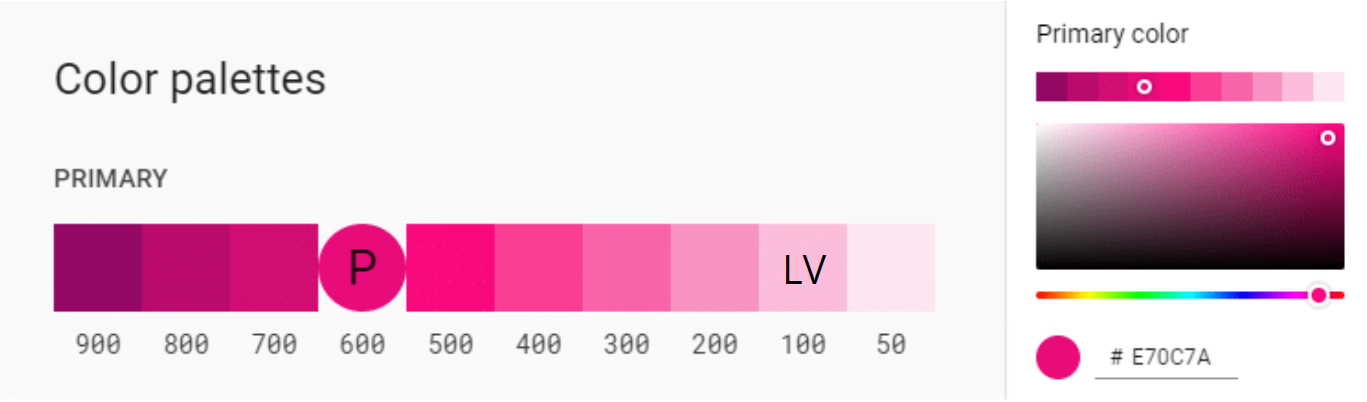
\includegraphics[width=0.8\textwidth, frame]
                            {./Med_Fidelity/Med_Report/images/colour_med.PNG}
                            %{./images/colour_med.PNG}
                        \caption{Colour Palette - Medium Violet Red [58]}
                    \end{figure}
                \end{itemize}

            \item Typography
                \begin{itemize}
                    \item Use popular font: The only font used throughout the app is 'roboto'. It is the default font for Android and many Google services [55]. The colour of the font is either the primary, white or grey depending on the background.
                    \begin{figure} [H]
                        \centering
                        
\includegraphics[width=0.8\textwidth, frame]
                            {./Med_Fidelity/Med_Report/images/font.PNG}
                            %{./images/font.PNG}
                        \caption{Font - Roboto}
                    \end{figure}                    
                \end{itemize}

            \item Iconography
                \begin{itemize}
                    \item Use industry standards metaphors: The appearance of the icons is in-line with material design where possible [59]. Some of these icons take advantage of closure in Gestalt's theory (users complete borders themselves) [40, 51]. The only icon that had to be sourced elsewhere was the scales for the compare feature.  
                    \begin{figure} [H]
                        \centering
                        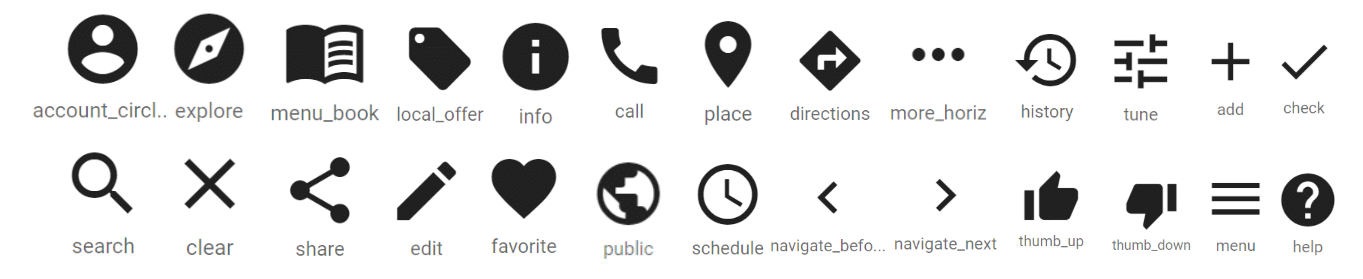
\includegraphics[width=0.9\textwidth, frame]
                            {./Med_Fidelity/Med_Report/images/material_icons.PNG}    
                            %{./images/material_icons.PNG}
                        \caption{Icons - Material Design [59]}
                    \end{figure}   
                \end{itemize}           

            \item States
            \begin{itemize}
                \item Hierarchical visuals (colour, text) - Titles and buttons should be large and primary coloured, to contrast against other elements to allow quick access [3].
                \item Highlight active interfaces - Ensures tabs are coloured when selected to make it clear to users the current page they are on.
            \end{itemize}

            \item Navigation
            \begin{itemize}                
                \item Bottom navigation bar - Provides access to 3-5 top-level destinations. This allows quick movement between screens [4]
                \item Navigation tabs - Used within the restaurant hierarchy to replicate the bottom bar to enable later navigation but for peer related content [4]. Also supports users mental models of tabs [45].
                \item Elements are consistent and locked - Follows the Gestalt principle of continuity [40, 51].
                \item Access to desired buttons - Offer clear affordances, less movement between pages [36].
                \item Large buttons lose to action - Reduced errors and wasted time as per Fitts law [40, 53].
            \end{itemize}
                
            \item Communication 
            \begin{itemize}
                \item Icons accompanied by small text - Although selected icons should be popular metaphors, added text helps to reduce the cognitive load and assist first-time users [4].
                \item Avoid jargon - Everyone should be able to understand any text used throughout the application. For example LIST was not clear and has been amended to COMPARE [5].
                \item Limit number of options - Keep all tabs, dropdowns and menus to under 5 visible options so as not to overwhelm the user as per Hicks Law [40, 54].
            \end{itemize}
            
            \item Space 
                \begin{itemize}
                    \item Dropdown/hidden menus - Follow the Gestalt principle of proximity, dropdowns show that options are related to one another. This promotes customisation and reduced cognitive load by allowing user to only see what is relevant to them [40, 64].
                    \item Keep interface elements to a minimum - Reduces the amount of space taken on the screen so overcrowding doesn't occur. White space is a friend [47].
                    \item Overlays - When elements are selected use an overlay with action buttons as proximity indicates these action are related to the selected according to Gestalt principle of proximity [39, 51]. This also takes advantage of the technique of progressive disclosure by keeping screen elements to a minimum and hidden until needed [5].
                \end{itemize}
            \item Time
                \begin{itemize}
                    \item Minimise user input - Stepping through should be quick and since on mobile typing only increases frustration and so should only be when absolutely required.
                    \item Don't overload with options - Hicks law makes it clear that users only want a select number of options to choose from [40].
                \end{itemize}
                   
           \end{itemize}    

    \subsubsection{System Requirements}
    From the initial research there were six system requirements identified that were implemented in the low fidelity prototype. For this next iteration, several of the requirements will remain the same:
    \begin{enumerate}
        \item Promote existing deals - Users are informed of whether an option is in their budget.
        \item Editable and shareable list - User needs a way to review their options.
        \item Restaurant information - Information to make an informed decision.
    \end{enumerate}      

    The requirements 'Filter map and menu view' will be split into two separate requirements as the functionality and purpose were identified to be actually slightly different. The map view provides an overview of options that match the user's need, and while the menu also performs this action it is a narrower and more customised view of the particular restaurant. This not only requires the categorisation of the restaurant as a whole but also the individual factors of the menu (price, ingredients, etc). Therefore, the requirement 'Interactive Map' will be updated to include this preference filtering and a new requirement added to describe the menu filtering.
        \begin{enumerate}[resume]
            \item Interactive map filtered by preferences - All relevant information is available within application. \\
                \textit{This is supported by previous research and the evaluations confirmed that this is expected behaviour of an interactive map as all participants understood it was interactive and could select a restaurant [24].}
            \item Filter embedded restaurant menu by preferences - Make decisions without navigating to another graphic/page. \\
                \textit{As per the initial research users almost always look at the menu beforehand and use apps to avoid navigating between different websites for information [24]. However, all users weren't aware in the low fidelity prototype that the menu was filtered and embedded but supported the idea [17].}
        \end{enumerate}

    The 'Recommend to a friend' requirement will also be split into two, as there are actually two separate requirements being compartmentalised into one; word of mouth recommendations and user tracking. 
        \begin{enumerate}[resume]
            \item Recommend to a friend - Remove focus from reviews and encourage user interaction. \\
                \textit{As per the initial research, users rarely leave reviews [24]. From the evaluations, most users commented that they would this word-of-mouth recommendation system as it is simple and it improves their experience [15].}
            \item Track user history - Remember preferences and customise experience. \\
                \textit{Users expected that they had access to their history and that they would be able to save their preferences for later use, especially since the application would be used weekly [24].}
        \end{enumerate}
 
    \subsubsection{Personas}
    To summarise and empathize with the users of the system, four personas have been developed. Each of these personas represent a different type of user to provide an overview of each group's expectations, use cases and highlight the most important functionality they need [67, 72]. There is a typical user as well as one at each end of the extremes (low and high use) and a user who requires the use of niche elements (dietary and planning). Each persona has a name, photo, life goal, blurb, quote relating to the system and an overview of their characteristics (employment, demographic, relationship status, income, interests, use of the system, restrictions, favourite food, age) [33]. The full breakdown of each persona can be viewed in \hyperref[sec:B.1]{Appendix B.1}.
    \begin{figure} [H]
        \centering
        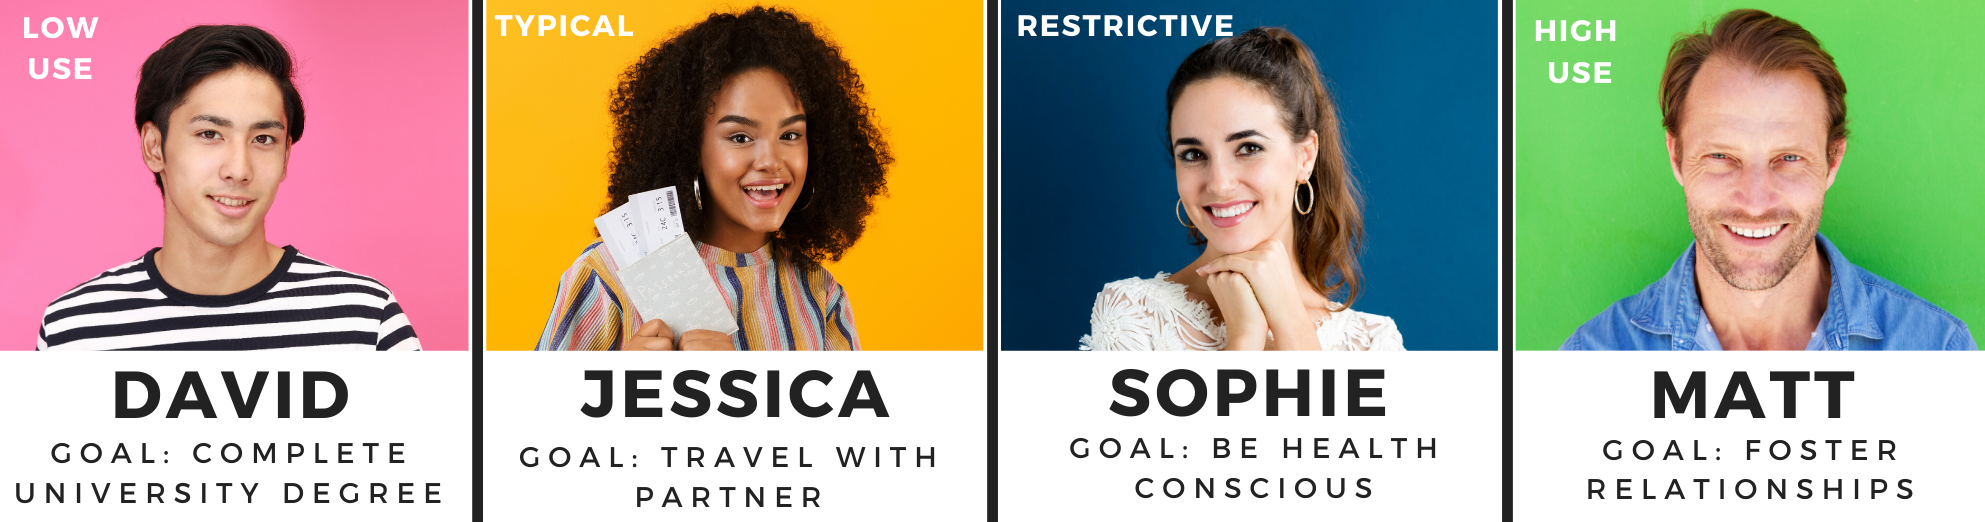
\includegraphics[width=0.9\textwidth, frame]
            {./Med_Fidelity/Med_Report/images/personas_overview.PNG}  
            %{./images/personas_overview.PNG}
        \caption{Personas Overview}
    \end{figure} 
    
    These personas were developed by reviewing the initial research of the application (both desk research and interviews) and the participants of the low fidelity evaluations to refine 'Who is the user?' and 'What is important to the user?' [24]. First need to look at the characteristics identified to describe the behaviour of the users:
        \begin{itemize}
            \item Who? Everyone eats out so personas are all in different age demographics, relationships, employment and income brackets.
            \item What? From the interviews, all 'sometimes' try new places so the personas are mixed. 
            \item When? Users range from eating out at least once per week up to four times per week so each user falls under a different number.
            \item Where? Anywhere, all like options
            \item Why? To share experience with others, so 3/4 of the personas always eat with others.
        \end{itemize}

    Also as identified in the initial research and confirmed by the low fidelity evaluations, there are six factors that are important to the user [24]. Each of these factors are covered by the features of the application. Each persona encompasses three of these factors in their decision process and eating out behaviours.
    \begin{center}
    \begin{tabular}{|l|c|c|c|c|}   
        \hline  
        Factor                                                          & David & Jessica& Sophie   & Matt \\
        \hline \hline
        Matches dietary \textit{(2/12 participants had dietary concerns)}&      &       & Yes       &   \\
        \hline
        Choose by craving \textit{('Taste' is most important factor)}   &       & Yes   &           & Yes \\ 
        \hline
        Word-of-mouth \textit{(91\% based on recommendation)}           &       &       & Yes       & Yes \\ 
        \hline
        Located nearby \textit{(1/3 mentioned as part of decision)}     & Yes   &       &           & Yes \\ 
        \hline
        Menu online \textit{(50\% always, 50\% sometimes look before)}  & Yes   & Yes   & Yes       &  \\
        \hline
        Deal or low cost \textit{(3rd most important factor)}           & Yes   & Yes   &           &  \\
        \hline
        \end{tabular}
    \end{center}
    
 

    \subsubsection{Interaction Scenarios}
    For each of the created persona's a storyboard of their typical interaction with the system was sketched. These scenarios communicate the subsets of user behaviour of the system to assist with ensuring all users needs are met and that the design of the system supports these expectations [33]. Each scenario has 11 slides and uses the template supplied by NNGroup with rough sketches and simple explanations. The scenarios range from unflawed or expected use of \textit{foodie} to challenges and frustrations with existing applications to represent a range of cases. There are four scenarios, all of which can be found in \hyperref[sec:B.2]{Appendix B.2}.
        \begin{enumerate}
            \item David - Student Deals: David wants to eat out with friends but wants to find the cheapest option. He uses Google Maps to look nearby but has to go to each restaurant's website to to view the deals. He struggles to remember all the deals and places he has looked at and the text conversation with his friends is just a mess of links and names. It takes over 20 minutes to find somewhere.
            \item Jessica - Hump Day: Jessica doesn't feel like cooking and so she wants to send some good value options to her partner. She regularly uses the Foodie app and has a list of favourites. She checks which one has a good deal and matches her craving to add to her comparison list. She sends these options to her partner, who in turn remembers somewhere he has been wanting to try and edits the list to send back to her. This place looks great so they decide to go here and Jessica saves it for next time too.
            \item Sophie - Busy Planner: Sophie has a busy day on the road tomorrow so she needs to plan what she is going to have for lunch. This is her least favourite task of planning as she has to look through lots of images of menus on the Zomato app to find what matches her diet. Then she reads through long reviews to get a sense of the place before writing it down in her diary for tomorrow. When tomorrow comes she will decide and have to get directions on Google Maps.
            \item Matt - Lunch at work: Matt is at work and is craving pizza for lunch. He wants to pick somewhere nearby that is preferably recommended by friends. He doesn't like to waste time deciding so he uses the Foodie app since he can filter by pizza and location on the first page and get a quick glance of what his friends think. 
        \end{enumerate}

    \subsubsection{UX Goals}
    When determining the 'success' of the user experience, according to NNGroup, it is important to 'focus on outcomes not the features' [46]. Rather than focus on the service the application is offering, focus on the problem that this application is solving. The problem is that no existing solutions give users what they actually want (the benefits); options to dine out with others based on personal preference (craving, dietary), nearby location and word-of-mouth recommendations.

    These UX Goals were developed by identifying the main user needs, from previous evaluations and research, and then selecting content and functionality requirements to meet them. The goals use SMART principles and together cover all systems requirements [41]. Each goal is a real-world end state that users want to reach [71]. The full details of the UX goals, including their source, measures and link to requirements, can be found in \hyperref[sec:B.3]{Appendix B.3}. 
        \begin{enumerate}
            \item I want to dine out at places that match my dietary requirement.
            \item I want to eat what I am craving.
            \item I want to choose where to eat based on my location. 
            \item I want to view the menu of the restaurant as it relates to me before going there.
            \item I want to learn about the relevant deals of a restaurant.
            \item I want access to the basic information of a restaurant.
            \item I want to compare a variety of restaurants at once.
            \item I want to share the experience of dining out with friends.
            \item I want to dine out at restaurants that have been recommended by word-of-mouth.
            \item I want to re-visit restaurants that I enjoyed.
            \item I want to find new places to eat out.
            \item I want to dine out in my budget.
            \item I want to decide where to dine out in less than 20 minutes.
            \item I want support restaurants without having to leave long reviews.
        \end{enumerate}

% 3.2.2 MEDIUM FIDELITY PROTOTYPE
\subsection{Medium Fidelity Prototype}
Taking into consideration the revised requirements as outlined from the results of the low fidelity prototype evaluations a medium fidelity prototype was created. Figma was chosen due to its browser-based interface, easy-to-use design, prototype functionality and popularity in the UX world [74]. Colour, icons and basic functionality has been implemented. The icons were created using logomkr [75] and any images are sources from the open-source photo collection on canva [73].

    \subsubsection{Interface Design}
    To align with the design principles any metaphors that didn't previously match the material design icons will be updated (Google Maps pin, compass, menu, coupon). Overall the updates ensure user's have clear understanding and awareness that:
        \begin{itemize}
            \item the shareable comparison list is a main feature with clear guidance to get there and understanding of its purpose. $\dashrightarrow$ Change LIST to COMPARE and update 'bookmark' metaphor to 'scales'. For the 'add to compare' icon, enlarge it, add this text and move it to the main area on restaurant page.
            \\ \textit{This will help David with finding options that he can share with his friends instead of having to remember them separately.} 
            \item both the map and menu are filtered by their personal preferences with the ability to expand or minimise these options as needed. $\dashrightarrow$ Add filter bar to MENU page, add shading to selected filters \\ 
            \textit{This will solve Sophie's frustration of wanting to look through multiple menus for her diet without navigating between websites.}
            \item recommendations are by word of mouth, with the option to view all responses as well. $\dashrightarrow$ Add text 'friends' next to recommendations, add option to view all reviews. \\
            \textit{This will save Matt time as he highly values the opinions of friends and wants to make a quick decision.}
            \item they have access to basic information of a restaurant on every relevant page. $\dashrightarrow$ Add overlay with more action icons when select from compare list \\
            \textit{This will assist Jessica with wanting to use her list of saved restaurants as her method of search to send to her partner to view.}
        \end{itemize}        
        
        The below is the interface of the medium fidelity prototype, with any relevant updates outlined. Also note, the application now has a name; foodie. It is simple and fun. It will replace APPNAME in the top navigation bar. 
            \begin{figure} [H]
                \centering
                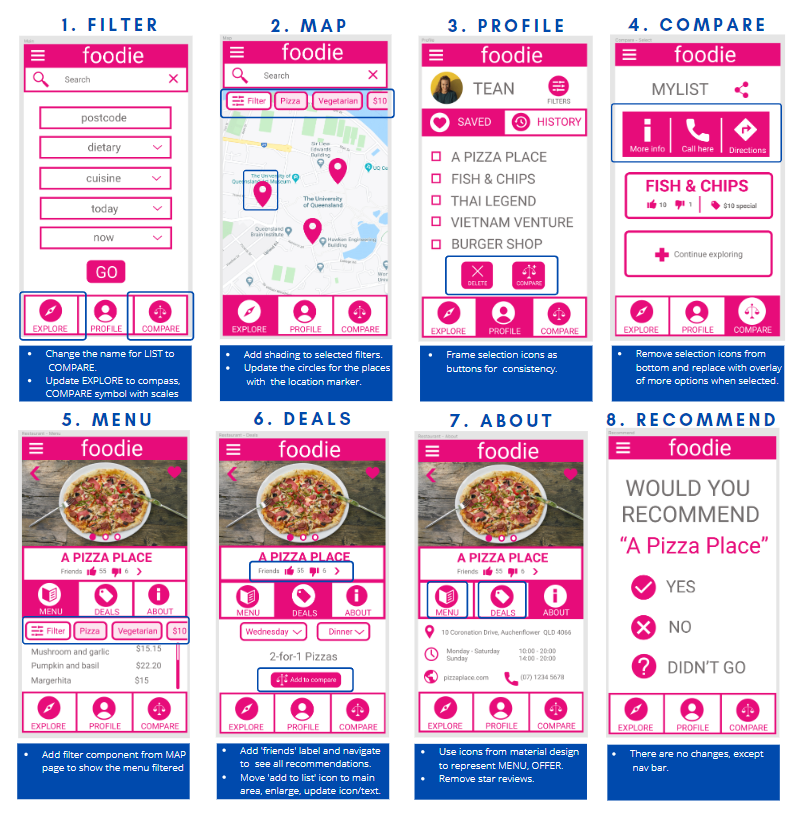
\includegraphics[width=0.9\textwidth, frame]
                    {./Med_Fidelity/Med_Report/images/med_proto_notes.PNG}  
                    %{./images/med_proto_notes.PNG}
                \caption{Medium Prototype - Interface Modifications}
            \end{figure}   
        
        \subsubsection{Interface Functionality}
        Since this is the first digital version of the prototype, the same interaction as the low fidelity prototype was implemented (only one end option for each feature). The functionality at this time mainly includes the navigation between tabs. For the buttons, the 'GO', back arrow and 'continue exploring' navigates to the map, while 'Add to compare' to the compare list. There is also the ability to scroll through the menu once. 
        \begin{figure} [H]
            \centering
            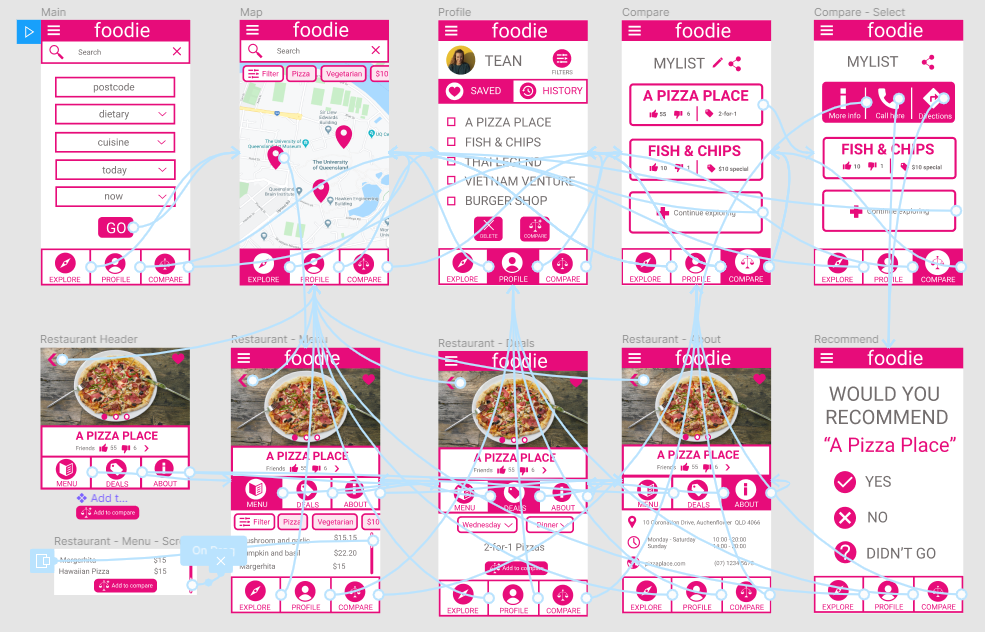
\includegraphics[width=0.9\textwidth, frame]
                {./Med_Fidelity/Med_Report/images/med_proto_func.PNG}  
                %{./images/med_proto_notes.PNG}
            \caption{Medium Prototype - Interface Functionality}
        \end{figure}


% 3.2.3 MEDIUM FIDELITY PROTOTYPE EVALUATION
\subsection{Medium Fidelity Prototype Evaluation}

    \subsubsection{Evaluation Methods}
    Instead of evaluating whether the application assists users with solving a problem the purpose of the evaluations of the medium fidelity is to determine the usability of the application which in turn contributes to shaping the user experience [57]. Any gaps between mental models in the low fidelity prototype have been amended for the medium fidelity prototype and it has been determined that this application is something users want, so now it is a matter of whether they can use it.  

    The think aloud evaluation method requires users to either complete a specific task or walk through all aspects of the application, whilst saying out loud everything they are thinking [42]. This method was chosen as it provides substantial qualitative feedback on the user's experience as it is happening in regards to their expectations of the system. Since the end goal for this application is the same for every user, deciding where to dine out, the process of deciding is different for every user with a wide range of approaches that can be taken with the system.

    The System Usability Scale (SUS) is a set of 10 questions, with both positive and negative responses, that provides a grade for the usability of the system. These questions are a popular staple of evaluation in the user experience industry as they are are cheap and quick process [66]. Since the user is only required to respond with a numerical value, the full picture of why and how users feel about a system may be missing. This is used to supplement the think aloud evaluation as it provides an overall quantitative picture of the user experience after an overload of qualitative feedback [66].
    
    After all evaluations have been completed, the raw data collected from the results of the SUS questionnaire will go through the following steps to effectively analyse the data and get a better understanding of users overall opinion of the systems usability. These steps will provide a SUS Score for each participant, as well as an average, which can be compared against the standard percentile ranks. Also, since the average of results can be skewed by outliers, a distribution of responses is generated which instead shows the median and interquartile range which is not affected by these outliers [35, 26].
        \begin{enumerate}
            \item Convert Raw Data: ODD = Response - 1, EVEN = 5 - Response
            \item Calculate SUS Scores: Total * 2.5 for each participant
            \item  Average for each question: Total / number of participants for each question
            \item Distribution of responses: Boxplot to show distribution of each question
        \end{enumerate}  

    \subsubsection{Evaluation Protocol}
    The purpose of this protocol, structure and consistency, is the same as the low fidelity prototype. The protocol can be viewed in \hyperref[sec:B.4]{Appendix B.4}. Also similarly, users are invited to a Google Form where all instructions, links and surveys are available to them. The form can be viewed in \hyperref[sec:B.5]{Appendix B.5}. After providing consent the user will be directed to an interactive prototype. Each page of the prototype is outlined by a typical android smartphone frame. The slides can be viewed in \hyperref[sec:B.1]{Appendix B.6}. 

    Users are asked to use the app as if they were a first time user interested in the app. They are given no specific task and are asked to speak all thoughts out loud with no interruptions from the evaluator. This is in-line with the Think Aloud evaluation method. In addition to taking note of their use and understanding of components of the prototype, the numerical measures (clicks, errors and time) for the UX goals will also be taken simultaneously. After the user has finished explaining each step of the system as they understand, users will be directed back to the Google Forms to answer the 'Survey Questions' to further measure the UX Goals. Each questions is rated out of 3 (don't agree, neutral, agree). Following these questions, the users will also complete the SUS questionnaire. This is simply the collection of raw data which will be analysed once all evaluations have been completed.
  
    For this evaluation, there are six participants in total. Three of the users will be brand new to the system, whilst the other two took part in the evaluation of the low fidelity prototype. This provides a balance of fresh eyes with no preconceived ideas who can comment on the basic flow of the application, and also those who already have a basic understanding who were able to evaluate if the changes made were appropriate and look at the application in more detail. The raw notes are in \hyperref[sec:B.7]{Appendix B.7}. 


    \subsubsection{Evaluation Results}
    The following provides an overview of the results and feedback from the evaluations and is separated by each persona's ability to complete their scenario. 
        \begin{enumerate}
            \item David - Student Deals
                \begin{itemize}
                    \item Today/now confusing, didn't understand the difference between the two $\dashrightarrow$ 2/5 user's mentioned.
                    \item Wants to be able to filter by price before getting to the map view $\dashrightarrow$ The poorest survey responses were to UX Goal 'I want to dine out in my budget'.
                    \item Liked that there was a dedicated page for deals, though wanted to be able to view this tab first (before menu).
                \end{itemize}

            \item Jessica - Hump Day
                \begin{itemize}
                    \item Went to the saved restaurant but couldn't go to the restaurant information page without adding to the compare list first $\dashrightarrow$ Poor response to 'I could easily access information when needed'
                    \item Tried to find an option to view all deals.
                    \item Wanted to be able to follow partner's saved places instead of just in the list. 
                \end{itemize}

            \item Sophie - Busy Planner
                \begin{itemize}             
                    \item Was able to filter by location, cuisine,  dietary and tomorrow which she felt made the search very custom.
                    \item Wanted to be able to save her preferences for later but couldn't find how to without assistance.
                    \item Still had difficulty finding how to add a restaurant to compare list though was quicker than previously $\dashrightarrow$ Poor responses to both time and survey results for UX Goal 'I want to compare a variety of restaurants at once.'
                    \item After finding places , wasn't sure if compare list was going to be able to save for the next day and wanted to be able to save for future trips. 
                \end{itemize}

            \item Matt - Lunchtime at work
                \begin{itemize}
                    \item Selected to filter by cuisine for the map, but wanted to be able tell which places were popular before having to click into each one
                    \item Once at the restaurant looked at the recommendations and could tell they were friends
                    \item Wanted to be able to go straight here without going to compare list, wanted a 'go here now' option $\dashrightarrow$ Poor response to 'I could easily access information when needed'
                    \item After going to the restaurant wanted to be able to recommend without having to open the app.
                \end{itemize}
        \end{enumerate}

    \subsubsection{Evaluation Analysis}
    The overall interaction of the app was much improved from the low fidelity prototype as users could now progress from the restaurant page to the compare list, and move from compare list to their next desired page (back or forward) without issues. This was confirmed by the positive responses and reduced number of errors to the related UX measures. The first step in understanding the data was to complete the data analysis steps of the raw data collected from the SUS questionnaire to calculate the scores and view the distribution. The data and graphs associated with the analysis of this raw data can be viewed in \hyperref[sec:B.8]{Appendix B.8}.

    In terms of usability, as per the SUS analysis the grading of the system overall was a low A with an above average score in the 82nd percentile. However, the scoring was as low as 62.5\% (C - below average) to 95\% (A - above average). 
    \begin{figure}[H]
        \centering
        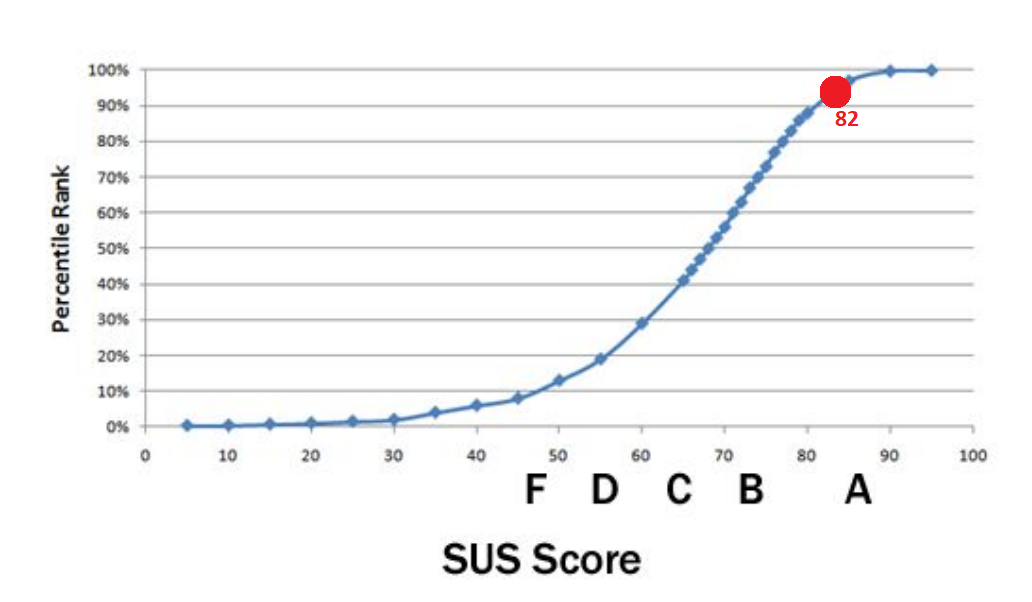
\includegraphics[width=0.5\textwidth, frame]
            {./Med_Fidelity/Med_Report/images/Med_SUS_Grade.PNG} 
        \caption{SUS Grade}
    \end{figure}   
        
   The lowest scoring questions was 'I thought there was too much inconsistency in this system' with an average of 2.8. The highest scoring question was (reverse) 'I think that I would need the support of a technical person to be able to use this system' with 3.66, closely followed with 'I found the system unnecessarily complex' with 3.5. All other questions were either rated overall 3.16 or 3.33. This suggests that the system is easy to use in terms of technical complexity, however there is still too much thought process involved with moving through the system.
   
   The think aloud evaluations identified that the main issue contributing to this inconsistency in this iteration was the availability of options for different actions. This also aligned with three UX goals not being met. The first UX goal not achieved is 'I want to dine out in my budget' which had to poorest response to survey questions. Users want to be able to filter by budget on the first page, and agreed the now option is redundant. The second UX goal is 'I want to compare a variety of restaurants at once', which caused the highest number of errors when moving from restaurant to compare. Users want a broader view of the places on the map view with differentiation of restaurants based on popularity before selecting an irrelevant restaurant (different colour or icons with legends). Also, although the time from restaurant page to compare list was greatly reduced, many of the users still had difficult finding the 'add to compare' button as it was often hidden. 

    The third UX goal that users was 'I could easily access information when needed' which was only met sometimes. Users want the ability to be assisted with going to a restaurant straight from the restaurant page without proceeding to the compare screen (more buttons). On the restaurant page no-one used the bottom tab and so instead this will be replaced by the popular action buttons. Additionally, users wanted to be able to access more information on the places recorded in their profile without having to add them to the compare list first. Most users commented they usually wouldn't select more than one restaurant at a time, so instead of checkboxes the same overlay as the compare page will be used (more info, add to compare and delete as the options).


    \end{document}
% 4 - HIGH FIDELITY PROTOTYPE SECTION
\pagebreak
% Setup
\documentclass[a4 paper, 12pt]{article}

% Title
\title{HIGH FIDELITY}

% Margins
\usepackage{geometry}
\geometry{margin=2cm}

% Images
\usepackage{graphicx}
\usepackage{float}
\usepackage[export]{adjustbox}
\setlength{\intextsep}{5pt plus 2pt minus 2pt}
\setlength\belowcaptionskip{0ex}
\usepackage[font=footnotesize,skip=2pt]{caption}

% Paragraph
\setlength{\parindent}{0em}
\setlength{\parskip}{1em}

% Text Formatting
\usepackage[utf8]{inputenc}
\usepackage[english]{babel}

% List spacing
\usepackage{enumitem}
\setlist{noitemsep, topsep=0pt}
\setlist[enumerate]{parsep=5pt} 

% Text Color
\usepackage{xcolor}

% Hyperlinks
\usepackage{hyperref}
\hypersetup{
    colorlinks=true,
    linkcolor=black,
    filecolor=black,      
    urlcolor=blue,
}

% Appendix
\usepackage{appendix}

% Include pdf
\usepackage{standalone}
\usepackage{pdfpages}

% Borders
\usepackage{mdframed}

% Symbols
\usepackage{amssymb}

\usepackage{multicol}

\usepackage{tabulary}
\usepackage{array}
\newcolumntype{L}{>{\arraybackslash}m{4cm}}
\newcolumntype{V}{>{\arraybackslash}m{6cm}}



\definecolor{mygreen}{HTML}{008037}
\definecolor{myblue}{HTML}{004AAD}
\definecolor{myorange}{HTML}{FF914D}
%%%%%%%%%%%%%%%%%%%%%%%%%%%%%%%%%%%%%%%%%%
\begin{document}
    
\section{Iteration 3 - High Fidelity Prototype}

    % 3.3.1 REVISED REQUIREMENTS
    \subsection{Revised Requirements/Conception Design}

    \subsubsection{System Concept Statement}    
    The following metaphors will be applied/added to this next iteration.
        \begin{itemize}
            \item cross $\dashrightarrow$ rubbish bin: Update to be consistent with industry standard.
            \item tuning $\dashrightarrow$ cog: The 'tune' metaphor did not match the users' mental models for setting default preferences. Tune metaphor remains for filtering. 
            \item home: User's considered the filter page the main page and consistently wanted to return here. \textit{(Participant 2: "looking for home button in the top bar to go back" [20])}
            \item floppy disk: Need a familiar metaphor for added 'saving' functionality
            \item arrow arched to the left: Undo
            \item rubbish bin with three lines: For remove all functionality on default preferences.
        \end{itemize}

        \begin{figure} [H]
            \centering
            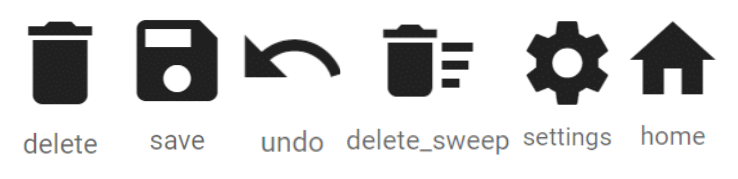
\includegraphics[width=0.5\textwidth, frame]
                {./High_Fidelity/High_Report/images/high_icons.PNG}  
                %{./images/high_icons.PNG}
            \caption{High Prototype Metaphors}
        \end{figure}  

    \subsubsection{Design Principles}

    A couple of the design principles that were not being met in the previous iteration are not being handled according to users. 
    \begin{itemize}
        \item Encourage collaboration - Users had no issues this iteration with viewing recommendations, recommending a visited place and sharing the compare list.
        \item Be familiar - There was no gap in mental models of any of the metaphors in this iteration.    
    \end{itemize}
       
    The following design principles have still not been adhered to in a satisfactory manner, causing continued issues for users.
    \begin{itemize}
        \item Customisation opportunities - Users had difficulty finding how they could set default preferences. This will be made clearer this iteration by updating the metaphor to a cog and the name to 'default preferences'. Users also wanted to be able to use their saved list to search and so an overlay will be introduced with more actions [68].
        \item Immediate access to actions - While users now had more action options on the compare page they also expected this overlay on other lists (saved/history). A similar overlay of actions will be added here. Also users wanted to be able to go straight to a place from the restaurant page so an action bar will replace the main bottom bar as it was not used. This position at the bottom of the screen ensures the easiest and quickest access for the users on mobile [4].
        \item Fluid navigation - There were still too many steps between pages, particularly for users who wanted to be directed straight to a restaurant without using the compare feature. A directions and call action will be added to the new action bar on the restaurant page.
        \item Clear direction \& guidance - The 'add to compare' button and favourites button were still hidden for many users. Both of these actions will be included in the action bar.
    \end{itemize}
    
    Two new design principles will be introduced to assist with resolving issues identified in the medium fidelity prototype.
        \begin{itemize}            
            \item Purposeful movement - Users noted that were a number of times where they had to navigate through various pages to complete a simple task. For example, to go to a restaurant users need to arbitrarily choose a place on the map, add this restaurant to the compare list, select the compare tab, choose the restaurant from this list then select directions/call. To assist with meeting this design guideline an overview of restaurants using icons will be added to the maps as well as a bar on the action page to allow users to go straight to a restaurant.
            \item Consistency - The colours of icons was not consistent which caused confusion and errors from the users. For this iteration, a focus on consistency across the application will be applied, including both visual (colours) and functional (interactive elements) consistency [5]. To achieve this, dark pink fill will represent active states, fark pink outline will represent clickable buttons and the light pink fill will be when an action/button has been selected.
        \end{itemize}

    \subsubsection{System Requirements}
    As per the evaluations, it is evident that all system features are important to the range of users and all will be carried forward into this next iteration. However, for the requirement 'Track user history - Remember preferences and customise experience' this will be now split into three parts as the customisation of the application has more expectations from the user than originally anticipated.
        \begin{itemize}
            \item Track user history - Easily re-visit restaurants. \\
            \textit{This feature now specifically focuses on user's desire to be able to re-visit restaurants they have been too before as demonstrated by the interest in this feature during the medium evaluations. Additionally, the initial research states that while users eat out at least twice a week, they try new places sometimes leaving potentially have that time for places they love.}
            \item Remember preferences - Shortcuts for expert users. \\
            \textit{During the medium evaluations the ability to set preferences was not made obvious, despite user's enquiring if there was a feature to be able to save for later}            
            \item Favourite restaurants - Alternative way to search for options. \\
            \textit{The capabilities of this feature are essential to Jessica and the clear definition provides expert users with more functionality. Also, in general users spend over 15 minutes searching through various options and don't want to repeat this process each time if avoidable.}
        \end{itemize}

    \subsubsection{Informed Models}
    There are no changes to the personas or interaction scenarios. 
    
    \subsubsection{UX Goals}  
    From the initial research and medium fidelity analysis, a number of the UX goals were not met adequately in the previous iteration.
        \begin{itemize}
            \item I want to re-visit restaurants that I enjoyed: User's did not have access to view more information about places in their history. 
                \begin{itemize}
                    \item \textit{Participant 2 \& 3: "I expected to be able to filter by history and use this to search options too." [9, 10]}
                    %\item \textit{Initial Research: All responded they try new places 'sometimes' which leaves remainder of time for places been before. [24]}  
                \end{itemize}            
            \item I want to dine out in my budget: The option to filter by budget was hidden and user's could not find it without assistance.
                \begin{itemize}
                    \item \textit{Participant 1 \& 2: "Want to be able to filter by price here but cant see that option.. was looking for it first" [19,20]}
                    %\item \textit{Initial Research: Cost is the 3rd most important factor. [24]}
                \end{itemize}            
            \item I want to decide where to dine out in less than 20 minutes: There is no information about a restaurant before selecting on a map increasing the time to decide. 
                \begin{itemize}
                    \item \textit{Participant 4: "Looking for what is most popular, wondering for a way to see where I been before quickly [22]}
                \end{itemize}            
            \item I want to compare a variety of restaurants at once: The 'add to compare' button was hidden on the restaurant page, so users weren't aware this goal could be met or it was difficult to find. 
                \begin{itemize}
                    \item \textit{Participant 2 \& 5: "can't find the add to compare option" [20, 23]}
                \end{itemize}            
        \end{itemize}

    Also, from the medium prototype evaluations and interaction scenario analysis, there are three desires/expectations from users that did not match any of the existing UX goals. 
        \begin{itemize}
            \item I want to use my favourites to choose a restaurant.  
                \begin{itemize}
                    \item \textit{Participant 2 \& 3: "I expected to be able to filter saved and use this to search options too." [20,21]}
                    \item \textit{Jessica (scenario): Wants to be able to use her saved list as primary search feature}
                \end{itemize}
            \item I want to visit a place without comparing options. 
                \begin{itemize}
                    \item \textit{Participant 3: "want to go straight to a restaurant without adding to compare" [21]}
                    \item \textit{Matt (scenario): Wants to go to first best place.}
                \end{itemize}
            \item I want to save my preferences for next time. 
                \begin{itemize}
                    \item \textit{Participant 2: "not clear that can set defaults, but I would use this" [20]}
                    \item \textit{Sophia (scenario): Her diet doesn't change and setting her preferences would save her a lot of time.}
                \end{itemize}          
        \end{itemize}


% 3.3.1 REVISED REQUIREMENTS
\subsection{High Fidelity Prototype}
Using the medium fidelity prototype as a strong foundation and the updated conceptual design, further steps to improve the usability, and therefore user experience, of the application were applied to a high fidelity prototype [57].

    \subsubsection{Interface Design}
    These were the main issues from the medium prototype and how they will be resolved::
    \begin{itemize}
        \item Filter by budget hidden $\dashrightarrow$ Add price to main filter page \\
        \textit{- David now has clear option to filter by what is most important to him}
        \item Difficulty setting default preferences $\dashrightarrow$ Replaced the icon with settings metaphor and added text, setting preferences is same as default filter page. \\
        \textit{- Sophie can now save her diet for next time}
        \item No overview on map  $\dashrightarrow$ Add classification icons to markers on interactive map            
        \item Can't go to restaurant without using compare feature $\dashrightarrow$ Add icon options to be able to get the information to go directly to a restaurant without adding to compare list. \\
        \textit{- Matt can now choose in less time as desired with just one option.}
        \item Expected to be able to filter saved/history lists $\dashrightarrow$ Added filter bar to these page similar to the map and menu pages. 
        \item Can't use saved list to access restaurant information $\dashrightarrow$ Added option to go to restaurant page from saved list using overlay.  \\
        \textit{- Jessica can now utilise her saved list better.}
    \end{itemize}

    This is an overview of the updated prototype, with the important aspect changes outlined and explained visually. 
    \begin{figure} [H]
        \centering
        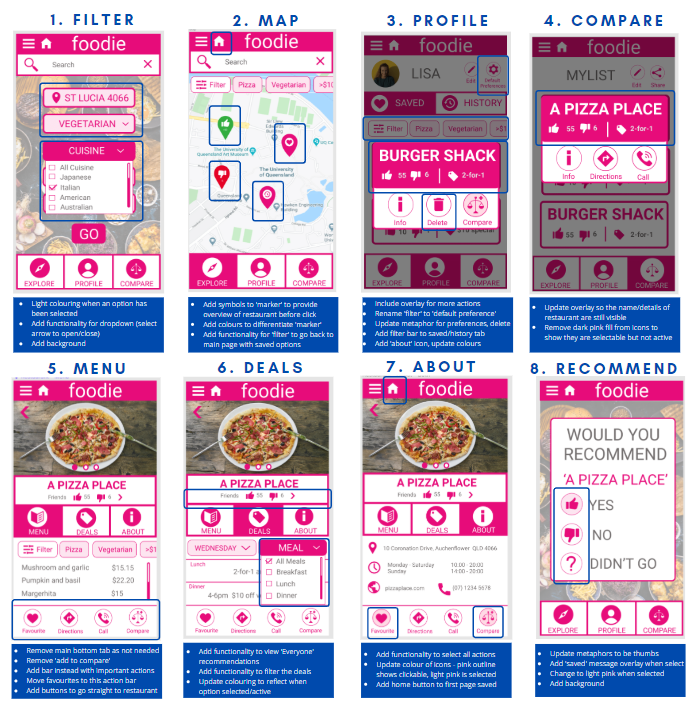
\includegraphics[width=\textwidth, frame]
            {./High_Fidelity/High_Report/images/high_proto_notes.PNG}  
            %{./images/high_proto_notes.PNG}
        \caption{High Prototype - Interface Modifications}
    \end{figure}  

    \subsubsection{Interface Functionality}
    Additional functionality has also been added to give the experts a more realistic experience of how the interface should behave.
    \begin{itemize}
        \item At least one option for each dropdown on main filter page.
        \item Basic preview of pages when adding default preferences.
        \item Change of state colour when adding a restaurant to compare or favourites.
        \item Preview of application status messages when saving a selection.
    \end{itemize}
    \begin{figure} [H]
        \centering
        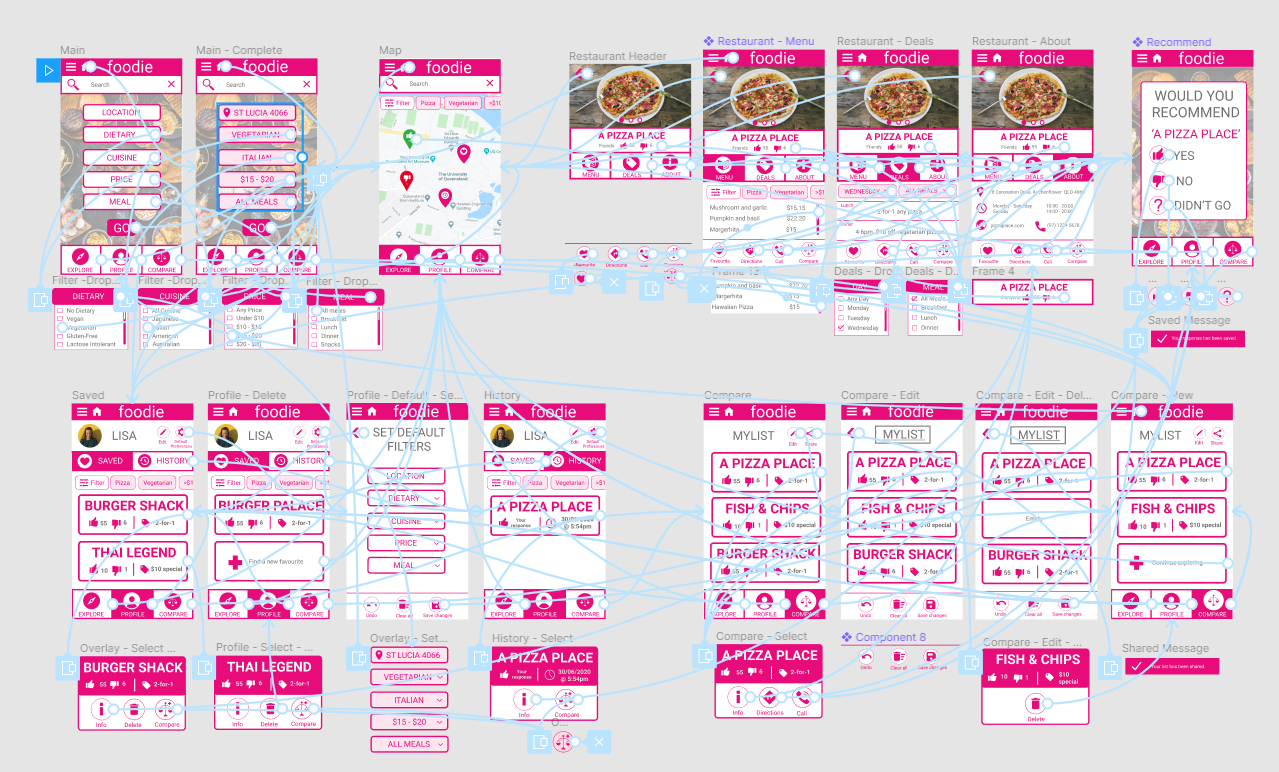
\includegraphics[width=\textwidth, frame]
            {./High_Fidelity/High_Report/images/high_proto_func.PNG}  
            %{./images/high_proto_notes.PNG}
        \caption{High Prototype - Interface Functionality}
    \end{figure} 



% High Fidelity Prototype Evaluation
\subsection{High Fidelity Prototype Evaluation}

    \subsubsection{Evaluation Methods}
    To effectively evaluate the high fidelity prototype, a heuristic evaluation will be undertaken. This method requires UI/UX experts to critically assess the interface of the application against a set of criteria to determine whether it meets a minimum standard of usability [42]. This criteria will be a list of 10 heuristics which have been specifically selected for this application. By using experts there are fewer ethical and practical issues, and their knowledge can provide key insights into the general expectations of usability the domain and identify potential issues when all functionality is properly implemented. However, it is important to keep in mind that there is an increased possibility of trivial issues being identified and some larger issues overlooked as they are not evaluating through the eyes of the user [43].    

    There are two preparation steps before starting the heuristic evaluation [34]. The first is to determine the features of the application. These have been outline and updated continuously in the system requirements sections of the reports. The second step is the choose the set of heuristics with these features in mind. By looking at the \textcolor{mygreen}{SMART} [56] and \textcolor{myblue}{Nielson 2001} [44, 61, 70]and \textcolor{myorange}{HOMERUN} heuristics [48], 10 heuristics were chosen as criteria to determine their usability [43].
        \begin{enumerate}
            \item \textcolor{mygreen}{Provide immediate notification of application status}: 
            This is a refinement of \textit{\textcolor{myblue}{Visibility of system status}}, which states 'The system should always keep users informed about what is going on, through appropriate feedback within reasonable time.' However, as this is a mobile application, the status must be immediate and due to screen size should be done non-intrusively where appropriate.
            \item \textcolor{mygreen}{Use a theme and consistent terms, as well as conventions and standards familiar to user}: This is a combination of \textit{\textcolor{myblue}{Consistency and standards (use platform conventions)}} and \textit{\textcolor{myblue}{Match between system and the real world (for user)}}. Essentially, users should know exactly what words and actions mean, and these phrases should be familiar to the user with information appearing in a logical order. Additionally, as this is a mobile application a theme should be used 'to ensure different screens look alike' and that the 'standards that users have come to expect in a mobile application' are used.         
            \item \textcolor{mygreen}{Prevent problems where possible; assist users should an error occur}: This is a combination of \textit{\textcolor{myblue}{Help users recognize, diagnose and recover from errors}} and \textit{\textcolor{myblue}{Error prevention}}. Error message should be clear and concise with solution suggestions, and even better 'prevents a problem from occurring in the first place'. It is essential that a mobile application 'is error-proofed as much as possible'.        
            \item \textcolor{myblue}{User control and freedom:} 'Users often choose system functions by mistake and will need a clearly marked "emergency exit" to leave the unwanted state without having to go through an extended dialogue. Support undo and redo.'        
            \item \textcolor{mygreen}{Each interface should focus on one task:} Due to the  of mobile application, This heuristic is unique to mobile application as a result of their use cases (frequent interruptions) and screen space (less cluttering). This means 'only having the absolute necessary elements onscreen to complete that task'.            
            \item \textcolor{myblue}{Aesthetic and minimalist design:} The original is \textit{\textcolor{myorange}{High quality content}} which is mainly for websites but highlights the important of providing functionality users want. The mobile equivalent is \textit{\textcolor{mygreen}{A visually pleasing interface}} and focus on the forgiveness of users if the interface is attractive. The 'attractiveness' of an application is a qualitative measure with different opinions. Instead this heuristic focuses on the aesthetic of the app by assessing whether it is minimalist, which is the preferred design of today's mobile Users [47].       
            \item \textcolor{myblue}{Recognition rather than recall:} The HOMERUN equivalent is \textit{\textcolor{myorange}{Ease of use}} which states that 'users need to be able to find the information they need quickly and easily. This is similar to \textit{\textcolor{mygreen}{Intuitive interfaces make for easier learning}}, which says similar for mobile interfaces in that they 'should be easy-to-learn whereby next steps are obvious'. Neither of these heuristics are clear about how the application should be achieving intuitiveness. Instead this heuristic focuses on minimises cognitive load by 'making objects, actions, and options visible' so that users dont need to remember each part of the process.
            \item \textcolor{mygreen}{Design a clear navigable path to task completion:} A more refined heuristic compared to \textit{\textcolor{myorange}{Relevant to users’ needs}} which measures whether the users are able to perform the task they want. This heuristic measures whether users are 'able to see right away how they can interact with the application and navigate their way to task completion'.     
            \item \textcolor{mygreen}{Allow configuration options and shortcuts:} A reworded revision of \textcolor{myblue}{Flexibility and efficiency of use}, it more appropriately identifies that the system should provide expert users with ability to tailor frequent actions. 
            \item \textcolor{mygreen}{Facilitate easier input:} This heuristic is unique to mobile applications in that it focuses on making it easy to input content from the perspective of a mobile device. 
        \end{enumerate}

    These were not chosen for this application:
        \begin{itemize}
            \item \textcolor{mygreen}{Display an overlay pointing out main features when appropriate or requested to help first-time users.:} This is similar to \textit{\textcolor{myblue}{Help and documentation}}, however there are no difficult elements of the application that need explaining and so no documentation is included for its use to be assessed by an expert
            \item \textcolor{mygreen}{Use camera, microphone and sensors to lessen user’s  workload:} The only sensors used in this application is GPS which is adopted from other applications and so there is no unique factors to asses for this application. According to research and existing solution no other sensors would be appropriate. 
            \item \textcolor{mygreen}{Cater for diverse mobile environments (lighting, ambient noise, gloves, etc):} At this stage there have been no accommodations made for different use case environments and so there is nothing for users to assess against this heuristic. 
            \item \textcolor{myorange}{Often updated, Minimal download time, Unique to the online medium, Net-centric corporate culture supporting site:} None of these heuristics are relevant to the mobile application or available to be assessed at this stage of prototyping.            
        \end{itemize}

    The are three stages of a heuristic evaluation; briefing session, evaluation period and debriefing session. During the evaluation period, experts go through the features of the application individually twice [43]. The first time is to get a feel and understanding of the interface, and the second time through is to focus on the specific features and make notes [62]. During this second pass, according to chapter 13.4.2 of The UX Book, each expert 'individually browses through each part of the interaction design, asking the heuristic questions about that part'. The expert takes note of where and how the heuristic has been violated, how this would cause usability issues for the user and the probable effect on the user. They also rate the severity of the usability issue choosing between two options for three factors; occurrence (common, rare), impact (low, high) and perseverance (very, not). The combination of these factors provide a severity rating (0 to 4), and the mean of at least three evaluators ratings is satisfactory to determine the seriousness of the usability issue [63]. The debriefing session is an extension that could be used to brainstorm ideas to resolve the violations [62].
        \begin{figure} [H]
            \centering
            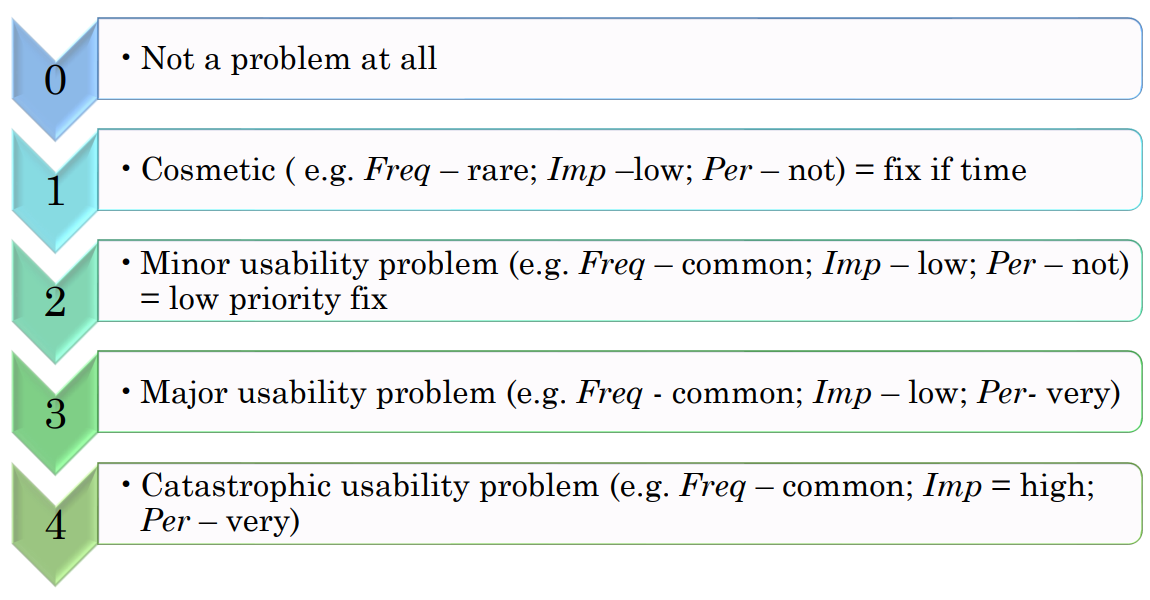
\includegraphics[width=0.6\textwidth, frame]
                {./High_Fidelity/High_Report/images/high_heuristic_severity.PNG}  
                %{./images/high_heuristic_severity.PNG}
            \caption{Heuristic Severity Ratings}
        \end{figure} 

    
    \subsubsection{Evaluation Protocol}
    The purpose of the protocol is the same as previous prototype evaluations. The protocol can be viewed in \hyperref[sec:B.1]{Appendix C.1}. To guide the experts through the three stages of the heuristic evaluation, after commencing the online call, the experts are provided with a link to a Google Forms. The form can be viewed in \hyperref[sec:C.2]{Appendix C.2}. This form  The first step is the briefing session where the expert is given an overview of the task and expectations, and asked to complete a consent form. The second stage is completing the heuristic evaluation. The expert is given a list of 13 tasks, each of which pass through every page and feature of the application. The expert is asked to complete each task at their own speed with guidance when/if and error occurs.  They are provided with a link to the high fidelity prototype on figma. The slides can be viewed in \hyperref[sec:C.3]{Appendix C.3}.
        
    After the user has completed all of the tasks and expresses they feel confident with the system they are directed back to the Google Forms to prepare for the second pass. During the second pass of the application, the expert is again asked to complete each of the tasks however this time they are to specifically evaluate the usability of the system against the chosen heuristics. There are ten heuristics that were identified as part of the preparation for the evaluation. On the Google Forms, the experts are provided a link to a Google Sheets where there is a tab called HEURISTICS which lists and describes each of the heuristics. In the sheet is a second tab for the expert to fill out their notes with the appropriate headings, including the severity rating factors. The tabs of the sheet can be viewed \hyperref[sec:C.4]{Appendix C.4}. The expert uses the same link to the prototype to evaluate each task against these heuristics. After they are satisfied they have identified all the current issues they are debriefed.
    
    This evaluation included 5 experts as this would identify at least 75\% of the evaluations [43]. One of the evaluators also took part in the low fidelity evaluation and another has participated in all three evaluations. This range of familiarity with the application may provide the identification of some unique issues and ensures that all previous issue were addressed. The raw notes are in \hyperref[sec:C.5]{Appendix C.5}. 

    \subsubsection{Evaluation Results}
    From the heuristic evaluation there were a range of issues identified. Where more than one evaluator has noted the issue the mean of the severity factor responses has been taken. Also in this case, the heuristic that was consistent amongst all answers was chosen or a judgment call was made for the most appropriate. \\
    \begin{tabular}{|V|l|l|l|l|}
        \hline
        \textbf{Issue} & \textbf{\#Experts} & \textbf{Heuristic} & \textbf{Factors} & \textbf{Severity} \\
        \hline \hline 
        \multicolumn{5}{|c|}{DROPDOWN} \\
            \hline \hline
            want to select whole box not just arrow & 4 & 10 & common,low,very & major \\    
            \hline
            want to select text not just box & 3 & 10 & common,low,very   & major \\
            \hline
            want to select anywhere to save option & 3 & 3, 8 & common,low,very  & major \\
            \hline \hline              
        \multicolumn{5}{|c|}{SAVED MESSAGE} \\
            \hline \hline
            save doesn't take user away from edit screen & 1 & 8 & common,low,very & major \\            
            \hline
            saved message has to be clicked out of and then back & 1 & 8, 4 & common,low,very & major \\
            \hline \hline
        \multicolumn{5}{|c|}{MAIN} \\
            \hline \hline
            reset option & 2 & 3 & rare,low,very & cosmetic \\
            \hline
            not clear what home icon refers to & 2 & 3 & rare,low,very & Cosmetic \\
            \hline \hline
        \multicolumn{5}{|c|}{COMPARE} \\
            \hline \hline
            too many steps to delete, edit page redundant & 4 & 8,3 & common,low,very & major \\            
            \hline \hline
        \multicolumn{5}{|c|}{RESTAURANT} \\
            \hline \hline
            no shortcut to compare/favourite & 2 & 9 & rare,low,not & cosmetic \\
            \hline 
            want to see more detail about reviews & 2 & 2 & common,low,not & minor \\
            \hline
            menu text area is small, lots scrolling & 1 & 7 & common,low,not & minor\\                
            \hline \hline
        \multicolumn{5}{|c|}{PROFILE} \\
            \hline \hline    
            not clear need to save defaults & 2 & 1,6 & common,high,very & catastrophic \\
            \hline
            cant add to favourite from history & 2 & 9 & rare,low,very & cosmetic \\
            \hline
            cant undo delete for saved & 1 & 4 & rare,low,not & cosmetic \\
            \hline
            not able to delete/modify history & 1 & 4 & rare,low,not & cosmetic \\
            \hline    
    \end{tabular}    


    %\begin{itemize}
        % \item DROPDOWN (Main, Default, Deals)        
        %     \begin{itemize}
        %         \item \textcolor{myblue}{want to select whole box not just arrow} \textit{(4 experts - heuristic 10 - common,low,very)}
        %         \item \textcolor{myblue}{want to select text not just box} \textit{(3 experts - heuristic 10 - common,low,very)}                
        %         \item \textcolor{myblue}{want to select anywhere to save option} \textit{(3 experts - 4, 10, 3,8 - common,low,very)}
        %     \end{itemize}    
        % \item MAIN
        %     \begin{itemize}
        %         \item reset option - [2 experts - 3 - rare,low,very] - Cosmetic
        %         \item home icon shouldn't be on this page - [1 expert - 3 - rare,low,very] - Cosmetic
        %     \end{itemize}
        % \item COMPARE
        %     \begin{itemize}
        %         \item too many steps to delete, edit page redundant [4 experts  - 4,9, 7,8, 2, 3 - rare, low, very]  - Cosmetic
        %         \item save doesn't take user away from edit screen [1 expert - 8,10 - common,high,very] - Catastrophic
        %     \end{itemize}
        % \item RESTAURANT
        %     \begin{itemize}
        %         \item no shortcut to compare/favourite [2 experts - 9 - (rare,low,not)] - Cosmetic
        %         \item want to see more detail about reviews - [2 experts - 2 - common,low,not] - Minor 
        %     \end{itemize} 
        % \item RECOMMEND
        %     \begin{itemize}
        %         \item saved message has to be clicked out of and then back [2 experts - 8, 1,4 - common,low,very] - Major
        %     \end{itemize}
        % \item HISTORY
        %     \begin{itemize}
        %         \item not able to delete/modify - 4 (rare,low,not) - Cosmetic
        %         \item cant add to favourite - [2 experts - 9 - rare,low,very]
        %     \end{itemize}
        %     \item SAVED
        %         \begin{itemize}
        %             \item cant undo delete - 4 (common,low,not)
        %         \end{itemize}
        %     \item DEFAULT
        %         \begin{itemize}
        %             \item not clear need to save - 6 (common,high,very), 1 (rare,high,not)
        %         \end{itemize}
        %     \item MENU
        %         \begin{itemize}
        %             \item text area is small, lots scrolling - 7 (common,low,very)
        %         \end{itemize}
        % \end{itemize}


    % \begin{itemize}
        % \item DROPDOWN (Main, Default, Deals)
        %     \begin{itemize}
        %         \item want to select text not just box- 3,10 (common,low,very), 10 (common,low,very), 10 (common,low,very)
        %         \item want to select whole box not just arrow - 8,10 (common,high,very), 10 (common,low,very), 10 (common,low,very), 10 (rare/low/very)
        %         \item want to select anywhere to save option - 4 (rare,low,very), 10 (common,low,very), 3,8 (common,high,not)
        %     \end{itemize}
    %     \item MAIN
    %         \begin{itemize}
    %             \item reset option - 3 (rare,low,very), 3,4 (rare,low,very)
    %             \item home shouldn't be here - 3 (rare,low,very)
    %         \end{itemize}
    %     \item COMPARE
    %         \begin{itemize}
    %             \item too many steps to delete, edit page redundant - 4,9 (rare,low,very), 7,8	(rare,high,very), 2 (common,low,very), 3 (rare,high,very)
    %             \item save doesn't take user away from edit screen - 8,10 (common,high,very)
    %         \end{itemize}
    %     \item RESTAURANT
    %         \begin{itemize}
    %             \item no shortcut to compare/favourite - 9 (rare,high,very), 9 (rare,low,very)
    %             \item want to see more detail about reviews - 2,10 (common,high,not), 2 (common,high,not)
    %         \end{itemize} 
    %     \item HISTORY
    %         \begin{itemize}
    %             \item not able to delete/modify - 4 (rare,low,easy)
    %             \item cant add to favourite - 9 (rare,low,very), 9 (rare,high,not)
    %         \end{itemize}
    %     \item RECOMMEND
    %         \begin{itemize}
    %             \item saved message has to be clicked out of and then back - 8 (common,low,very), 1,4 (rare,low,easy)
    %         \end{itemize}
    %     \item SAVED
    %         \begin{itemize}
    %             \item cant undo delete - 4 (common,low,not)
    %         \end{itemize}
    %     \item DEFAULT
    %         \begin{itemize}
    %             \item not clear need to save - 6 (common,high,very), 1 (rare,high,not)
    %         \end{itemize}
    %     \item MENU
    %         \begin{itemize}
    %             \item text area is small, lots scrolling - 7 (common,low,very)
    %         \end{itemize}
    % \end{itemize}


    \subsubsection{Evaluation Analysis}
     All of the heuristic violation results identified according to this sample of experts, so while approximately 75\% may have been collected there is potential that another set of the same evaluations with different experts could yield different results. Additionally, many of the issues identified were only identified by 1 or 2 experts which provides unreliable results. A further step that could be taken would be to recontact the experts with the entire list of issues and ask them to rate each one. This was not available at this time.  

     From the results there are four issues where their severity rating can be considered reliable (more than 3 experts), all of which have been identified as having a major market impact. This means they are 'important to fix, should be given high priority' [63]. The first two of these issues relate to the small area of selectability of the dropdown boxes and their content. These violate \textbf{heuristic 10} and do not align with Fitts law as larger buttons/selection area and proximity between selections is better for the user. The following two issues both violate \textbf{heuristic 3} and \textbf{heuristic 8} as they require unnecessary steps from the users and increase the chance of unresolved errors occurring. When selecting an option on a dropdown menu users have to be careful about how they choose to exit the overlay or their option will not be saved, and when deleted an option from the compare list users have to carefully complete at least four steps without warning if the sequence is not correct. These issues cause frustration and confusion for the user. All of these four issues will definitely need to be rectified in the next iteration due to their agreed consensus from experts as major issues.

     The remaining issues were only identified by one or two experts and so that severity rating is not entirely reliable. Looking at those rated by at least two experts, there are four cosmetic issues, one minor, and one catastrophic. Reviewing these violations objectively, these issues will be considered for the next iteration with lower priority than the major issues identified previously. The first issue has been labelled as catastrophic in violation \textbf{heuristic 1} and \textbf{heuristic 6}, which occurs on both the default preferences and edit compare list page. Experts noted that it was not clear that on these edit pages the changes needed to be saved as not only was there no response from the application when the pages weren't saved but this was not required for similar behaviour in other areas of the application. The minor issue violates \textbf{heuristic 2} and relates to the inability to view more information about reviews on the restaurant page when selecting the icons, despite this being an expected behaviour and functionality from other rating systems. The next two issues violate \textbf{heuristic 9}, firstly by not allowing users to add a visited restaurant to favourites easily and secondly by not providing accelerators to the favourite and compare list from the restaurant page for expert users [49]. The final two cosmetic issues relate to the violation of \textbf{heuristic 3} on the main page due to the absence of a reset button and the confusing presence of the home icon. 
          
     The final issues have only been identified by one expert and include two cosmetic, one minor, one major and one catastrophic. These will need further evaluation to determine their actual severity rating. At this time the two cosmetic issues violate \textbf{heuristic 4} and both relate to the profile page in that restaurants in the history cannot be delete/modified and there is no option to confirm or undo a deletion from the saved list. The minor issue is that the text of the menu is too small which may cause lots of scrolling and violates \textbf{heuristic 7}. The major and catastrophic issue are both identified by the same expert whom stated that the saved messages violate \textbf{heuristic 8}. The major issue is that when the saved message pop-up appears users must click outside of it and then the back arrow to go back, and the catastrophic issue is that after selecting saved the user isn't taken directly back to the previous screen. This is an example of the rating of one expert is unreliable as these appear to be less serious issues than presented given the impact of other issues. 

     The reliable major usability problems will be adjusted with high priority. This will resolve all of the violations of \textbf{heuristic 10}. For the unreliable issues from two experts the catastrophic issue will be given next priority followed by the minor problems. This will resolve all violations of \textbf{heuristic 1,2,6}. The cosmetic issues in this list will be handled if there is time, which will handle \textbf{heuristic 3,9}. The issues identified by only one expert will be rated further by at least one other expert before deciding, to determine the actual violation of \textbf{heuristics 4,7,8}. According to the results there is no violation of \textbf{heuristic 5}.

% \begin{itemize}
%     \item (1) Provide immediate notification of application status \& (6) Recognition rather than recall: Both violated once by the same issue which occurred on both the default preferences and edit compare list page. Experts noted that it was not clear that on these edit pages the changes needed to be saved as not only was there no response from the application when the pages weren't saved but this was not required for similar behaviour in other areas of the application.
%     \item (2) Use conventions and standards familiar to the user: Experts noted the inability to view more information about reviews on the restaurant page by selecting the icons. This is an expected behaviour and functionality from other rating systems. This is a minor issue so it is low priority.
%     \item (3) Prevent problems where possible; assist users should an error occur: The first relates to the absence of a reset option on the main page. The second issue was that the home icon is evident on the page despite this being the home page, potentially confusing users with what the icon then means. Also, users options are not saved unless they select arrow exactly.
%     \item (4) User control and freedom: This heuristic was violated on the profile page by 2 separate issues. The first is that once an option is deleted from the saved it cannot be undone if this was a mistake and the second is that the user is unable to delete/modify an option from their history if it is incorrect. 
%     \item (5) Each interface should focus on one task: This was the only heuristic that was not violated.    
%     \item (7) Aesthetic and minimalist design: This was violated on the menu page according to one expert who stated the text was too small which would be problematic if the menu was long due to extended scrolling.   
%     \item (8) Design a clear navigable path to task completion: This issue relates to the process of deleting an option from the compare list. Currently users must select 'edit', then select the option, then select 'delete' then save then back.  
%     \item (9) Allow configuration options and shortcuts: Firstly, experts noted that there was no way to get to the compare or favourites page after adding a restaurant without going back to the map. Secondly, a restaurant in the history list could not be added to favourites without searching for it again.  
%     \item (10) Facilitate easier input: The issues all relate to the selectability of the dropdown boxes and their content. Currently only selecting the arrow icon and the tick box exactly will open/select an option.     
%     \end{itemize}



\end{document}




\pagebreak
% NEXT STEPS
\section{Summary (Release 2)}
In summary, there have been three iterations of the human interaction cycle. The outcome of these cycles have been compiled and summarised for reference of progression. User research should be done at all stages so this is no way a complete list [46]. The final conceptual design (metaphors, system requirements, design principles, UX Goals) from these cycles can be viewed in \hyperref[sec:D.1]{Appendix D.1}. The progression of the prototype interface can be viewed in \hyperref[sec:D.2]{Appendix D.2}. Each iteration is denoted by a different colour; \textcolor{mygreen}{low}, \textcolor{myblue}{medium} and \textcolor{myorange}{high}. 

The next step would be to complete another iteration cycle. This would include updating the conceptual design (metaphors, system requirements, design principles), UX goals and prototype. Without going into full detail of these changes, the new metaphors to be introduced would be related to a refresh/reload action as well as repurposing the cross metaphor as the cancel option when checking user's navigation. A new design guideline would be introduced 'minimal effort' to ensure user's don't have issues with the selectability (particularly of dropdowns) again. There are a few system requirements that were previously mentioned by users and research that were beyond the scope of release 1. These include the ability to follow other users, save lists for future self use or or for others to view, and a voting system with the comparison list.

In order of severity ratings as outlined in the high fidelity evaluation analysis, these are ideas for changes that could be applied to the next prototype iteration only focusing on what can be improved with the conceptual design from release 1. 
\smallskip
    \begin{enumerate}[noitemsep,topsep=0pt]
        \item The whole box of a dropdown needs to be made selectable. $\dashrightarrow$ Fitts Law
        \item The text of options in the dropdown should be selectable. $\dashrightarrow$ Fitts Law
        \item Once an option has been selected in a dropdown users should not to worry about how they exit the overlay and should be saved no matter their next click. $\dashrightarrow$ Fitts Law
        \item Remove the edit action icon on the compare page. Instead a delete option, using the bin metaphor, will be added to the existing list of actions in the overlay when selecting an option on this page. This reduces the number of steps from 4 to 2 and replicates the same behaviour as the saved page. $\dashrightarrow$ Consistency
        \item Prompt user to save defaults if they haven't selected before exiting page.
        \item Support the display of more information when selecting the recommendations/reviews on restaurant page i.e. which friends voted.
        \item Remove the home button from the main page.
        \item Have a reset option as an icon the main page (less obvious than the GO button as it is less used) and when select prompt the user to confirm they want to reset.
        \item Add favourite action icon to overlay on history page.
        \item Add accelerator to favourite and compare buttons, long press to be directed straight there.        
    \end{enumerate}
    
    \begin{figure} [H]
        \centering
        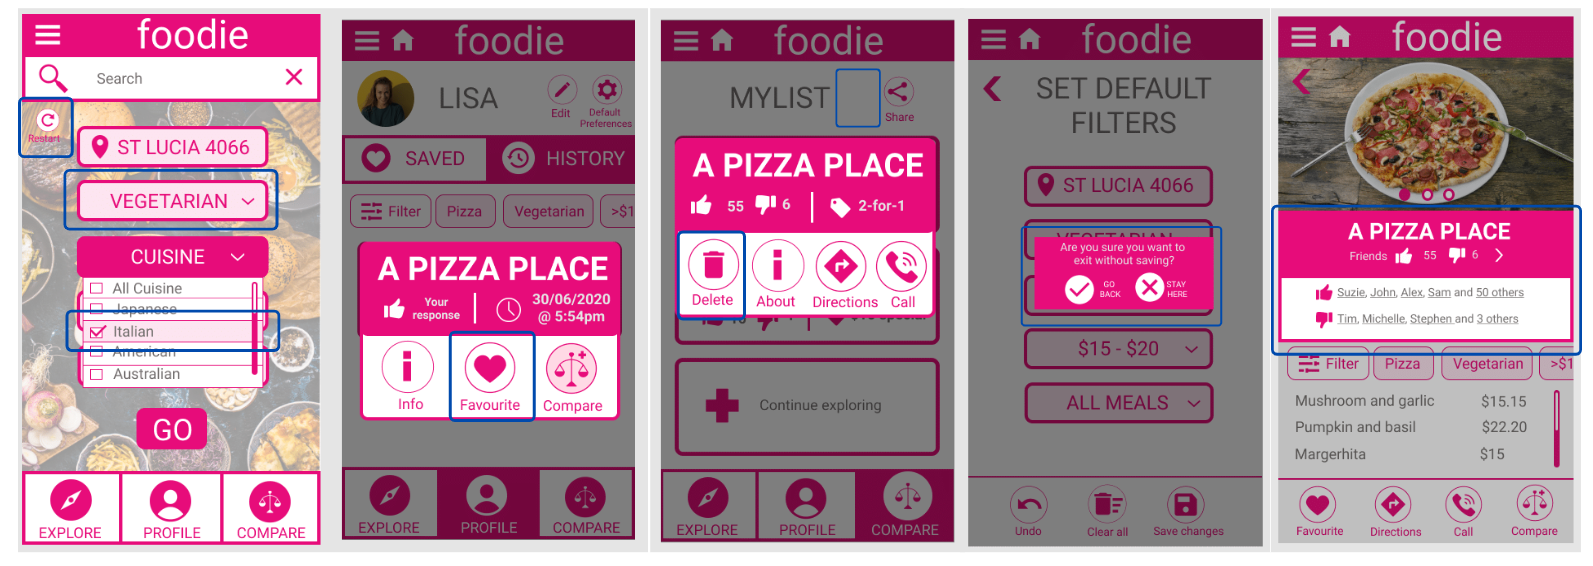
\includegraphics[width=0.9\textwidth, frame]
            {./Summary/next_prototype.PNG} 
        \caption{Release 2 Prototype}
    \end{figure}  

\pagebreak
% CONCLUSION
\section{Conclusion}
The foundation of this application came to fruition through the initial research (both desk and interviews) performed during the development of the mind map. From this research, \textit{Foodie} has been developed and refined through three iterations of the design process. Each step involved the creation/modification of the conceptual design which in turn was applied to the prototype and then tested through various evaluation methods (both user and expert based). In each iteration the gap between the gulf of execution and evaluation continued to close, mental models were better aligned, consistency throughout the system achieved, UX goals met and cognitive overload reduced using various techniques. Overall, while there are still improvements to be made to release 2, as briefly mentioned, the project started with identifying an issue and ended with a useable and accepted application. Users can now happily make the decision of where to dine out.

\pagebreak
% REFERENCES
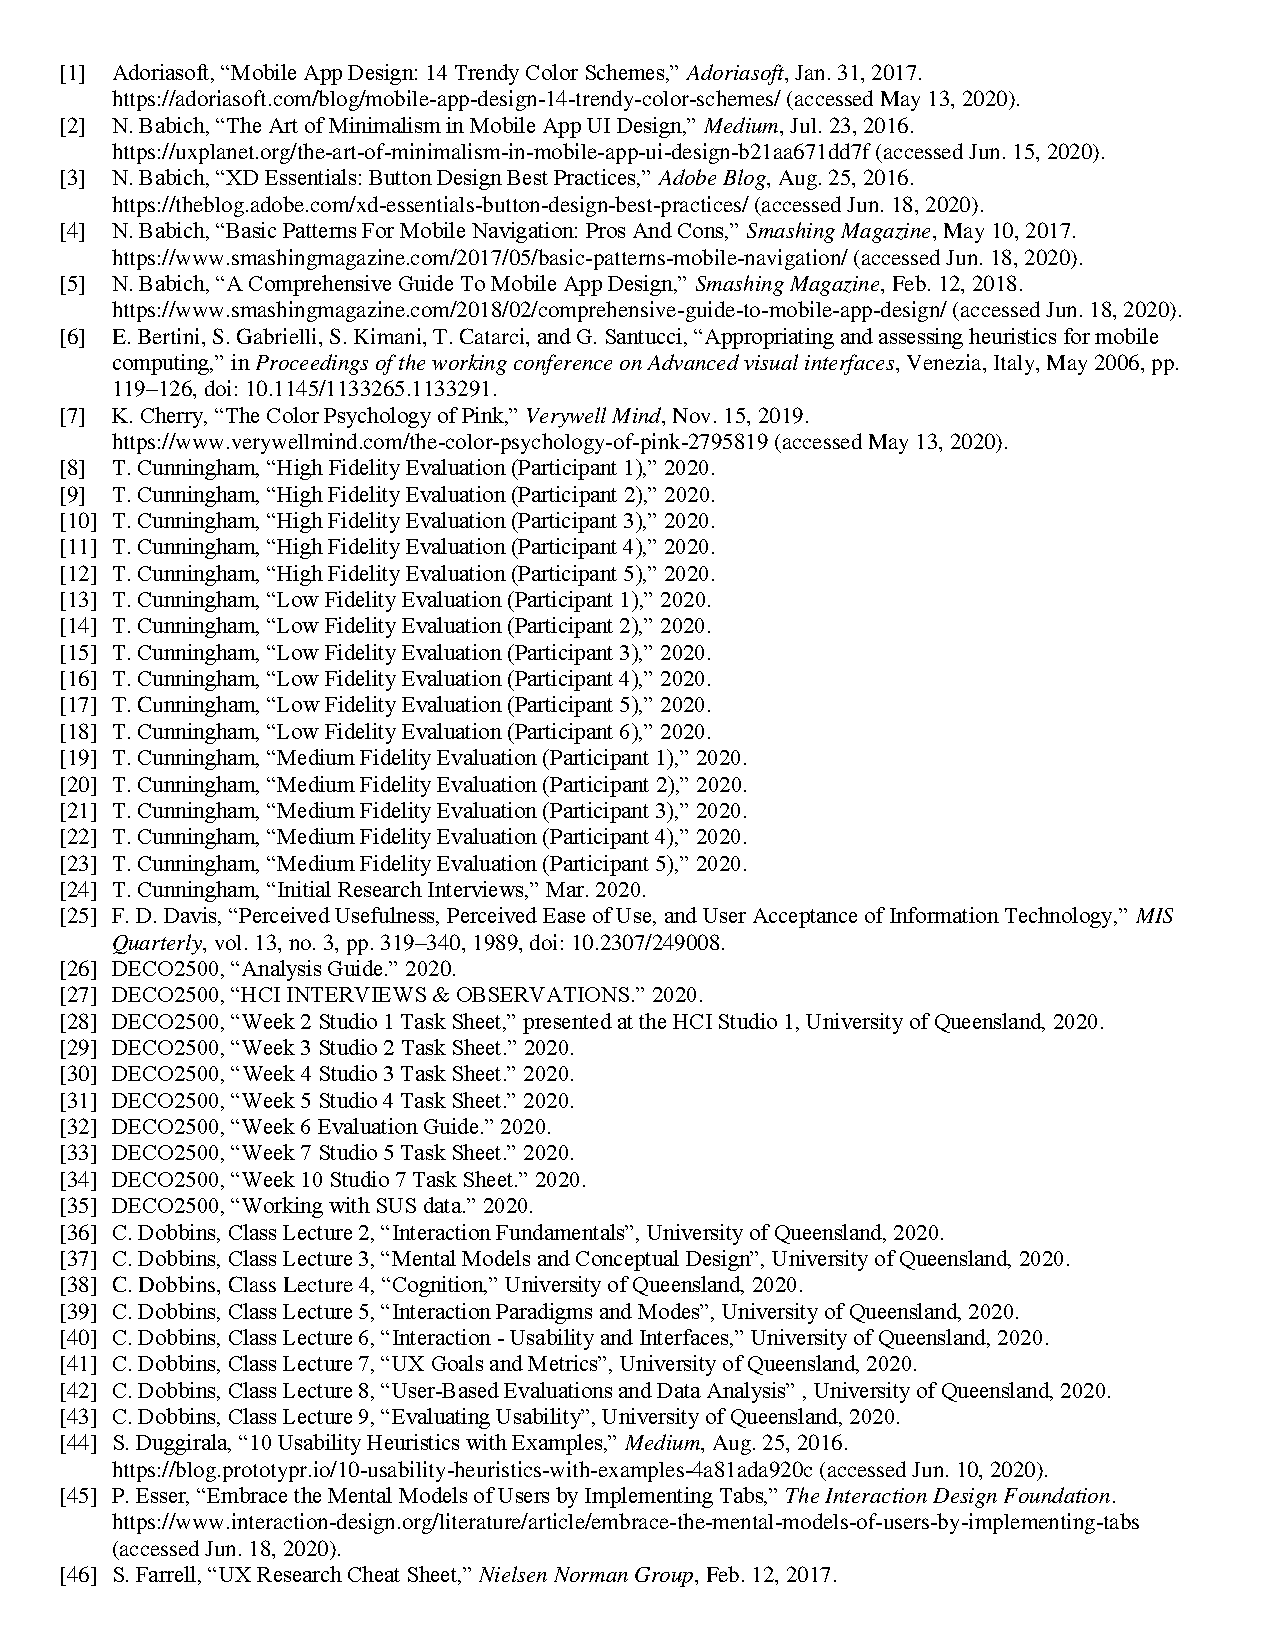
\includepdf[pages=1, pagecommand=\section{References}, offset=0 -0.5cm]{references.pdf}
\includepdf[pages=2-, offset=0 0cm]{references.pdf}



\appendix
\addappheadtotoc

% LOW FIDELITY 
% Title
\pagebreak
\begin{center}
    \vspace*{\stretch{0.7}}
    \Huge \textbf{Appendices}
    \section{Low Fidelity Prototype}
    \vspace*{\stretch{1}}
\end{center}

    % Evaluation Protocol
    \pagebreak
    % \subsection{Evaluation Protocol}
    % \begin{mdframed}[linewidth=2pt]
    %     \begin{center}
    %         \bigskip
    %         \Large \textbf{EVALUATION PROTOCOL\\
    %         Low-Fidelity Prototype}            
            
    %         \normalsize Tean-louise Cunningham
    %     \end{center}
    % % \documentclass[a4 paper, 12pt]{article}

% \title{EVALUATION PROTOCOL \\ Low Fidelity Prototype}
% \author{Tean-louise Cunningham (42637460)}
% \date{}

% \usepackage{geometry}
% \geometry{margin=2cm}

% \usepackage[utf8]{inputenc}
% \usepackage[english]{babel}
% \usepackage{xcolor}


% \setlength{\parindent}{0em}
% \setlength{\parskip}{1em}
%%%%%%%%%%%%%%%%%%%%%%%%%%%%%%%%%%%%%%%%%%
\begin{document}
\maketitle
\begin{center}
Complete a design walkthrough of low-fidelity prototype to identify gaps between conceptual and mental models.
\end{center}

\section*{PREPARATION}
Since this is an individual evaluation only myself and the participant will be involved. Therefore, I will be fulfilling the role of facilitation, observation, recording and interaction flow. The following materials will be prepared for the user prior to the evaluation.

\begin{enumerate}
    \item Electronic Consent form
    \item Paper Prototype
    \item Walkthrough Presentation Slides
    \item Questionnaire
    \item Google Forms
    \item Zoom software
\end{enumerate}

\section*{INTRODUCTION}

    \subsection*{Opening Statement}

        \textcolor{lightgray}{User has been sent a link with survey and instructions on Google Forms. User’s screen is being shared over an online conference call.}

        \begin{itshape}
            Thank you for taking the time today to provide some feedback on the early stages of a mobile application. The purpose of this app is to assist you with deciding where to dine out using an interactive map, filtered preferences and comparison feature.

            Today, I will be showing you the basic prototype to observe how you interact with it , to determine any functionality or design that is not intuitive, and whether it is achieving its purpose effectively for you as the user.
        \end{itshape}

    \subsection*{Consent}
        \begin{itshape}
            Before we get started, please read carefully through this consent form. It reiterates the purpose for today and how your data will be used. Your personal details will not be used directly in any way and all observations are of your interaction with the software only. If you like to proceed with contributing please fill out this form and upload with the given link.
        \end{itshape}

        \textcolor{lightgray}
            {User reads through and fills out consent electronically with provided link and uploads.}
        
        \begin{itshape}
            Thanks for filling that out, please save it on your computer for the time being. If it any time you don’t wish to continue just let me know and we will stop, and none of your feedback will be used.
        \end{itshape}

\section*{DESIGN WALKTHROUGH}
    \subsection*{Instructions}

        \begin{itshape}
            To get your feedback, I will be asking you to complete a specific task using the prototype. At any point you get stuck or are confused I may pause you for a moment to ask you some questions. I won’t be explaining or showing you how to use the system. The point of this exercise is to see what you, as a first time user, expect of the system and how you think it should flow.

            In a moment you will be able to view the paper prototype and move through the pages. Please interact with the application as if it was reactive. This means pressing everything that you normally would to complete the task. The more realistic your interaction with the prototype the better the feedback to know where to improve. 

            You will have 10 minutes to complete the following task. Any questions? 

            Please click on the link to the presentation. The task is to choose two places and decide between them where you would like to eat dinner tonight, takeaway of course. You can start.
        \end{itshape}

        \textcolor{lightgray}{The user confirmed they have no questions and is starting the task.  Record, observe and take detailed notes of their process.}

    \subsection*{Task Notes}
        These are the steps that the user should be going through to complete the task, and observations relating to each one that need to be taken note of.

        \begin{enumerate}
            \item Filter preferences: 
            This is the default page and so all users will start here.
                \begin{itemize}
                    \item Do they know how to filter?
                    \item Did they fill all of the filters out before proceeding?
                    \item Did they know how to get to the next page?
                    \item How long did it take to complete this page?
                \end{itemize} 
            \item Interactive Map:
            This is the page that follows the preferences page.
                \begin{itemize}
                    \item Were they able to select a restaurant?
                    \item Did they know the map was interactive?
                    \item Did they try to press any other buttons on the page?
                    \item How long did it take them to select a restaurant?
                \end{itemize}
            \item Restaurant Information
                \begin{itemize}
                    \item After selecting a ‘dot’ on the interactive map they will be brought here. 
                    \item How many of the cards did they select?
                    \item Did they understand the menu was filtered?
                    \item Did they know what all the icons meant?
                    \item Were they able to add a place to a list?
                    \item What information did they want to look at?
                    \item How long did it take them to move to another step?
                \end{itemize}
            \item List page:
            If a user selects the ‘List’ icon they will be brought here to compare.
                \begin{itemize}            
                    \item Did they get to this page?
                    \item Do they know how to select a decision?
                    \item Do they understand what to do next?
                    \item How long did it take the user to find out their was a list page?
                \end{itemize}
            \item Repeat: 
            Since the task is to select 2 places, users will need to repeat 2-5
                \begin{itemize}
                    \item Were they able to find out how to get back to previous steps?
                    \item Did they want to choose a second place?
                    \item How long did it take to figure out how to get back to the map?
                \end{itemize}
            \item Recommendation Page:
            After they have chosen a place and completed the task they will be nudged here.
                \begin{itemize}
                    \item Did they understand what was happening?
                    \item Did they know what they were suppose to do?
                \end{itemize}        
        \end{enumerate}

\section*{CO-DESIGN}

    \subsection*{Instructions}
        \textcolor{lightgray}{While completing the task the user encounters a problem and has taken more than 15 seconds to move to the next step, or they took an action expecting different functionality.}

        \begin{itshape}
        Please just pause for a moment:
            \begin{itemize}
                \item Do you understand what the next step is?
                \item What are you having trouble finding or understanding?
                \item Where/what do you think you should be able to find?
                \item How would you design this part?
            \end{itemize}
        \end{itshape}

        \textcolor{lightgray}{Show them the next step to continue the evaluation of the whole task.}


    \subsection*{Problem Notes}
        \begin{enumerate}
            \item Frequency
                \begin{itemize}
                    \item How many times did the user get stuck?
                    \item Were they able to move forward more times than they got stuck??
                \end{itemize} 
            \item Reason    
                \begin{itemize}
                    \item Did they get stuck because they didn’t understand the task?
                    \item Did they get stuck because of the design?
                    \item Was the flow confusing?
                    \item Was the order they expected?
                \end{itemize} 
            \item Next step    
                \begin{itemize}
                    \item After you showed the next step were they still confused?
                    \item Was the next step intuitive for them?
                \end{itemize} 
        \end{enumerate}

\section*{TAM EVALUATION}
    \subsection*{Instructions}
        \textcolor{lightgray}{The user has completed the task.}

        \begin{itshape}
            Thank you for completing the task. Now select to go back to the form. Finally, I have some questions to rate your experience and your  acceptance of this application. The purpose is to determine the perceived usefulness and ease of use, your attitude towards the app and intention to use.

            For each question choose a number between 1 and 4, with 1 being strongly disagree and 4 being strongly agree. Please answer honestly. I may follow up with additional questions where necessary. 
        \end{itshape}

    \subsection*{Questionnaire}
        \begin{enumerate}
            \item I can accomplish deciding where to dine out more quickly using this application (PU1)
            \item This application enables me to make better decisions about where to dine out. (PU5)
            \item Overall I find this application useful (PU6)
            \item It is easy to use this application to decide where to dine out (PEOU2)
            \item Overall I believe this application is easy to use (PEOU3)
            \item Overall my attitude towards this application I favourable (ATT3)
            \item I will use this application on a regular basis in the future (ITO1)
            \item I will strongly recommend others to use this application (ITO3)
        \end{enumerate}

    \subsection*{Questionnaire notes}
        The quantitative answers from the users will be saved on Google Forms which automatically calculates and graphs collected data. Additionally, any score that is not 4 (strongly agree) will be followed up with the following questions.

        \begin{itemize}
            \item Why did you give this score?
            \item What stopped you from scoring higher?
            \item         
        \end{itemize}


\section*{Conclusion}
    \begin{itshape}
        All done. Thank you so much for your time today. Just a reminder that if you would like to withdraw at any time, let me know and your data will not be used. Thank you for your time, it is greatly appreciated and your data is very valuable.
    \end{itshape}

\end{document} 
    % \end{mdframed}
    \includepdf[pages=1, 
                pagecommand=\subsection{Evaluation Protocol}, 
                width=\textwidth,
                height=\textheight,
                keepaspectratio, 
                frame, offset= 0 -1.5cm]
                    {Low_Fidelity/Low_Protocol/Low_Protocol.pdf}
                    \label{sec:A.1}
    \includepdf[pages=2-, 
                width=\textwidth,
                height=\textheight,
                keepaspectratio,
                frame, offset= 0 0cm]
                    {Low_Fidelity/Low_Protocol/Low_Protocol.pdf}

    % Google Forms
    \pagebreak
    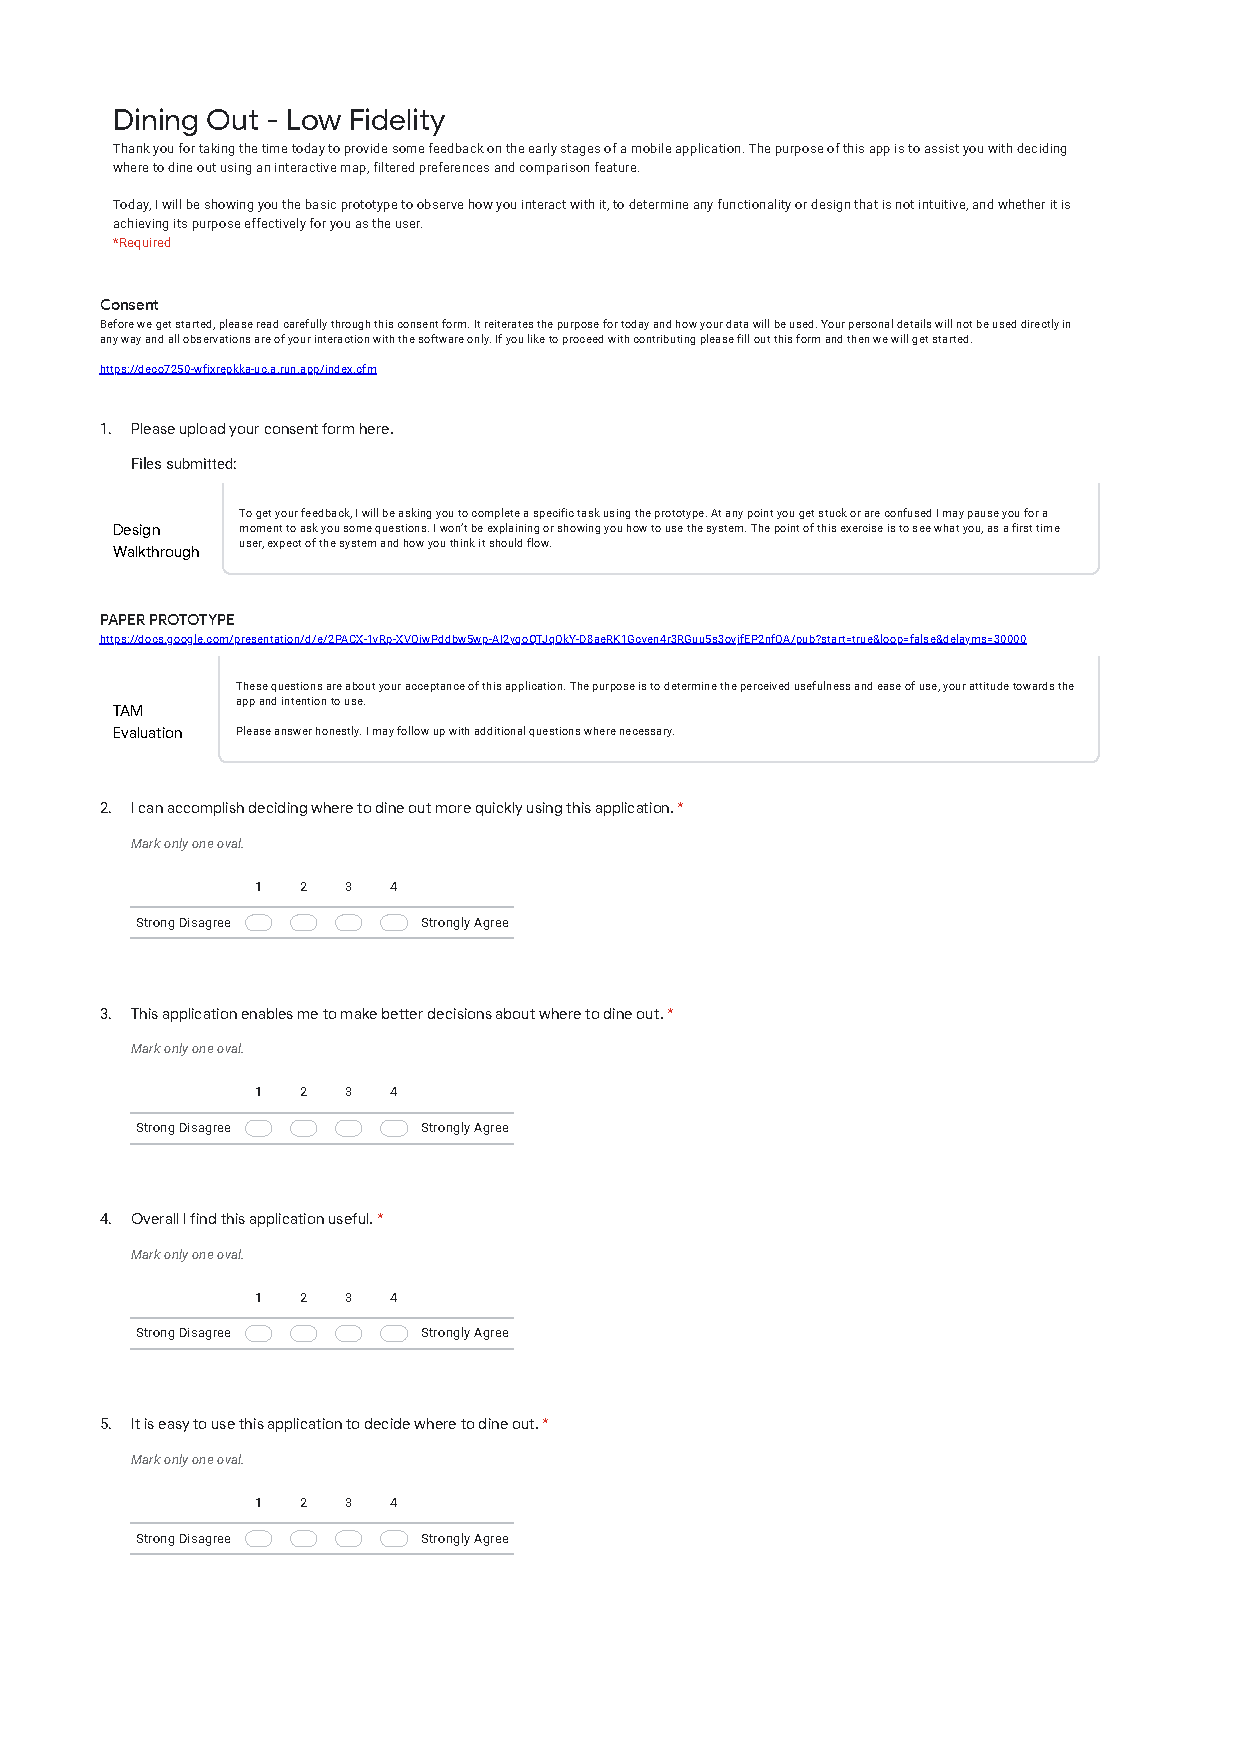
\includepdf[pages=1, 
                pagecommand=\subsection{Google Forms}, 
                width=\textwidth,
                height=\textheight,
                keepaspectratio, 
                frame, offset= 0 -0.5cm]
                    {Low_Fidelity/Low_Form.pdf}
                    \label{sec:A.2}
    \includepdf[pages=2-, 
                width=\textwidth,
                height=\textheight,
                keepaspectratio,
                frame, offset= 0 0cm]
                    {Low_Fidelity/Low_Form.pdf}

    % Presentation
    \pagebreak
    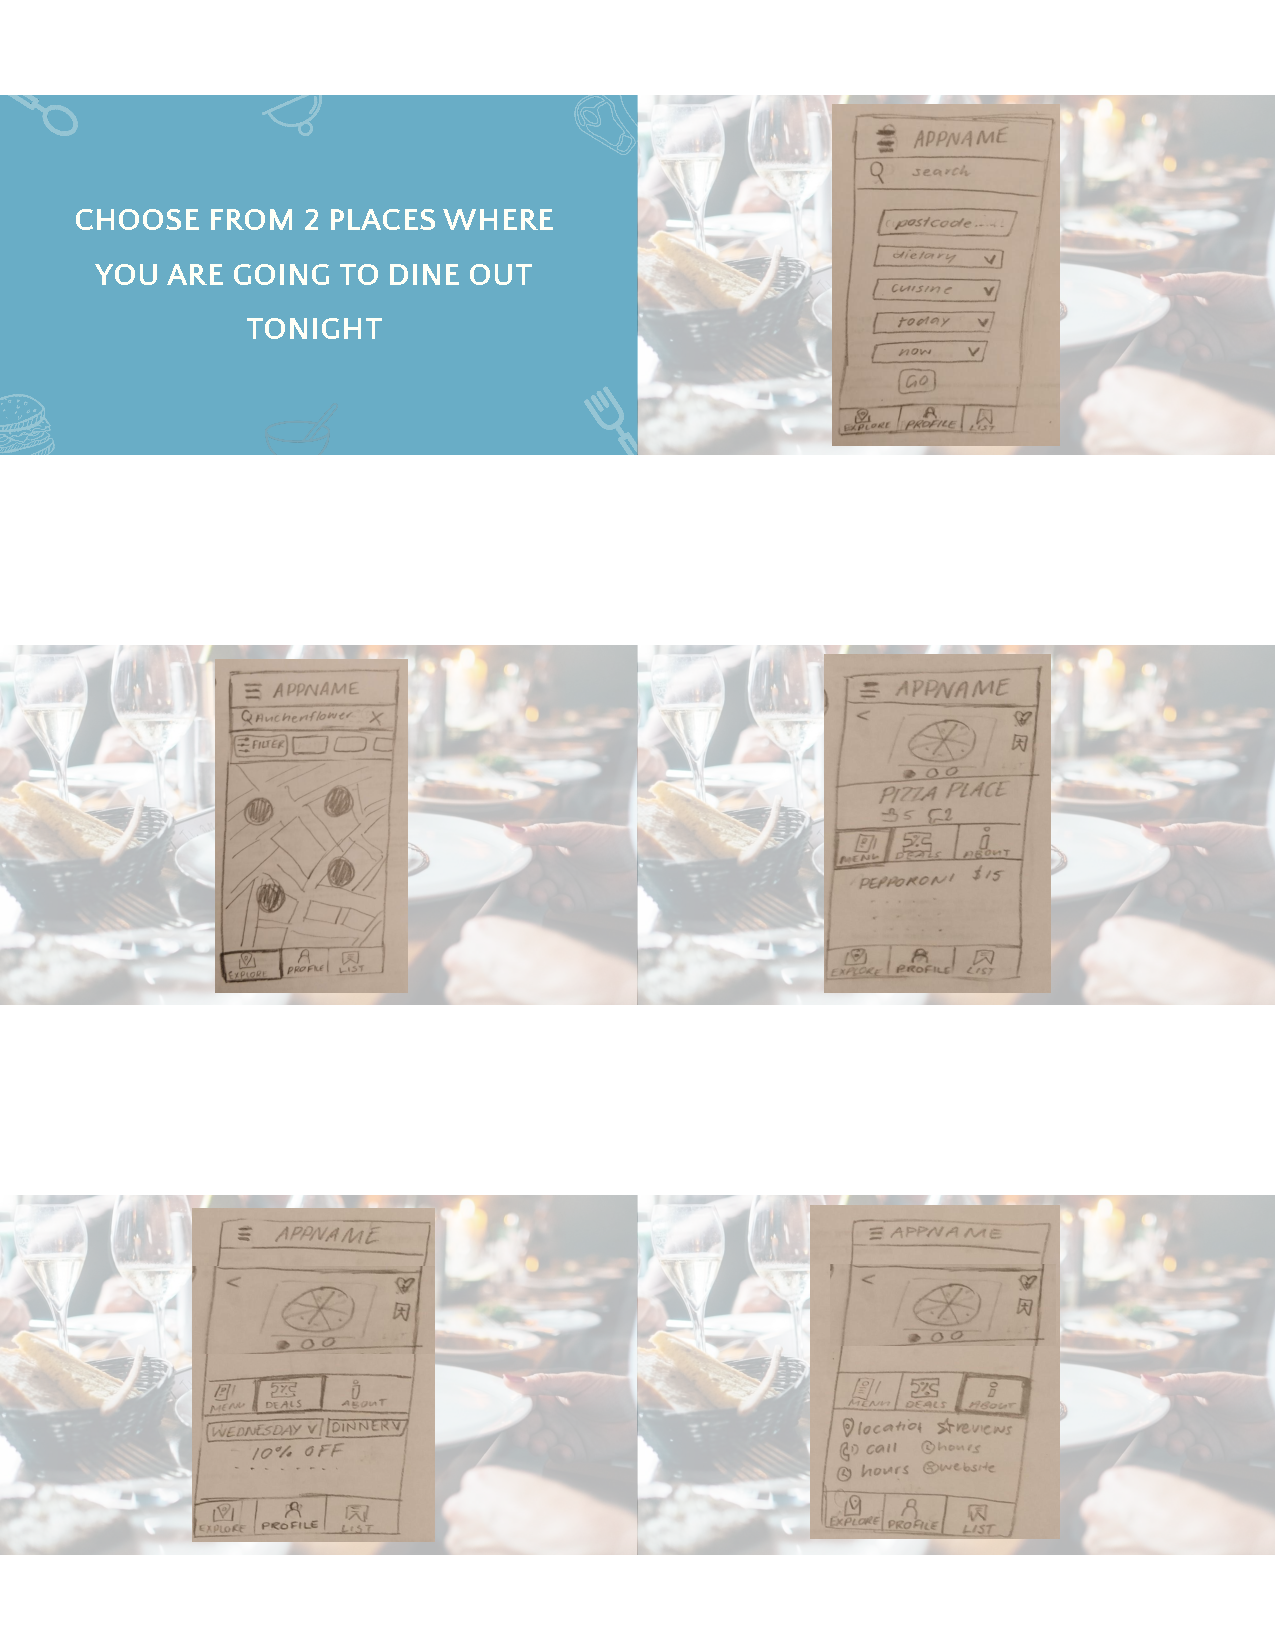
\includepdf[pages=1, 
                pagecommand=\subsection{Presentation}, 
                width=\textwidth,
                height=\textheight,
                keepaspectratio, 
                frame]
                    {Low_Fidelity/Low_Slides.pdf}
                    \label{sec:A.3}
    \includepdf[pages=2-, 
                width=\textwidth,
                height=\textheight,
                keepaspectratio,
                frame, ]
                    {Low_Fidelity/Low_Slides.pdf}

        % Questionnaire Results
        \pagebreak
        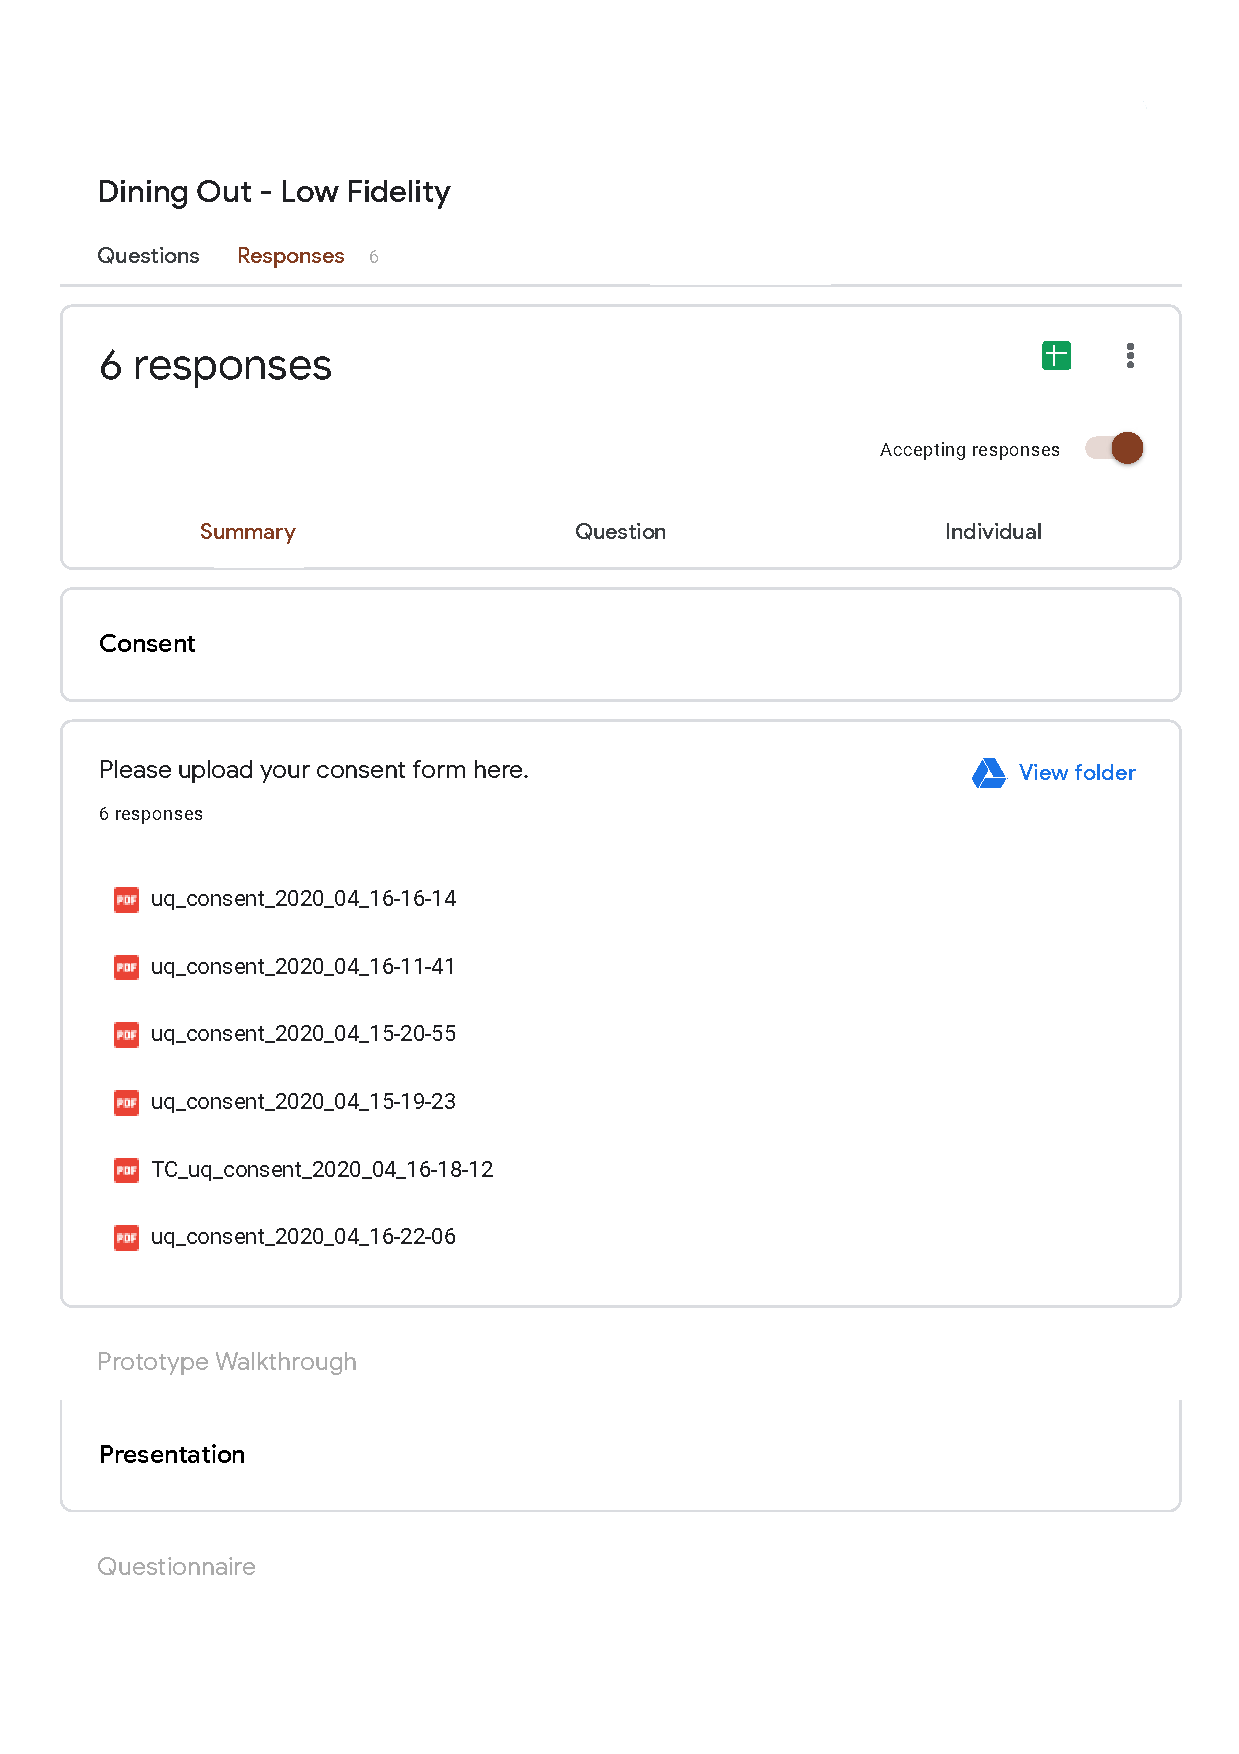
\includepdf[pages=1, 
                pagecommand=\subsection{Questionnaire Results}, 
                width=\textwidth,
                height=\textheight,
                keepaspectratio, 
                frame]
                    {Low_Fidelity/Low_Results.pdf}
                    \label{sec:A.4}
    \includepdf[pages=2-, 
                width=\textwidth,
                height=\textheight,
                keepaspectratio,
                frame, ]
                    {Low_Fidelity/Low_Results.pdf}

    % Notes
    \pagebreak
    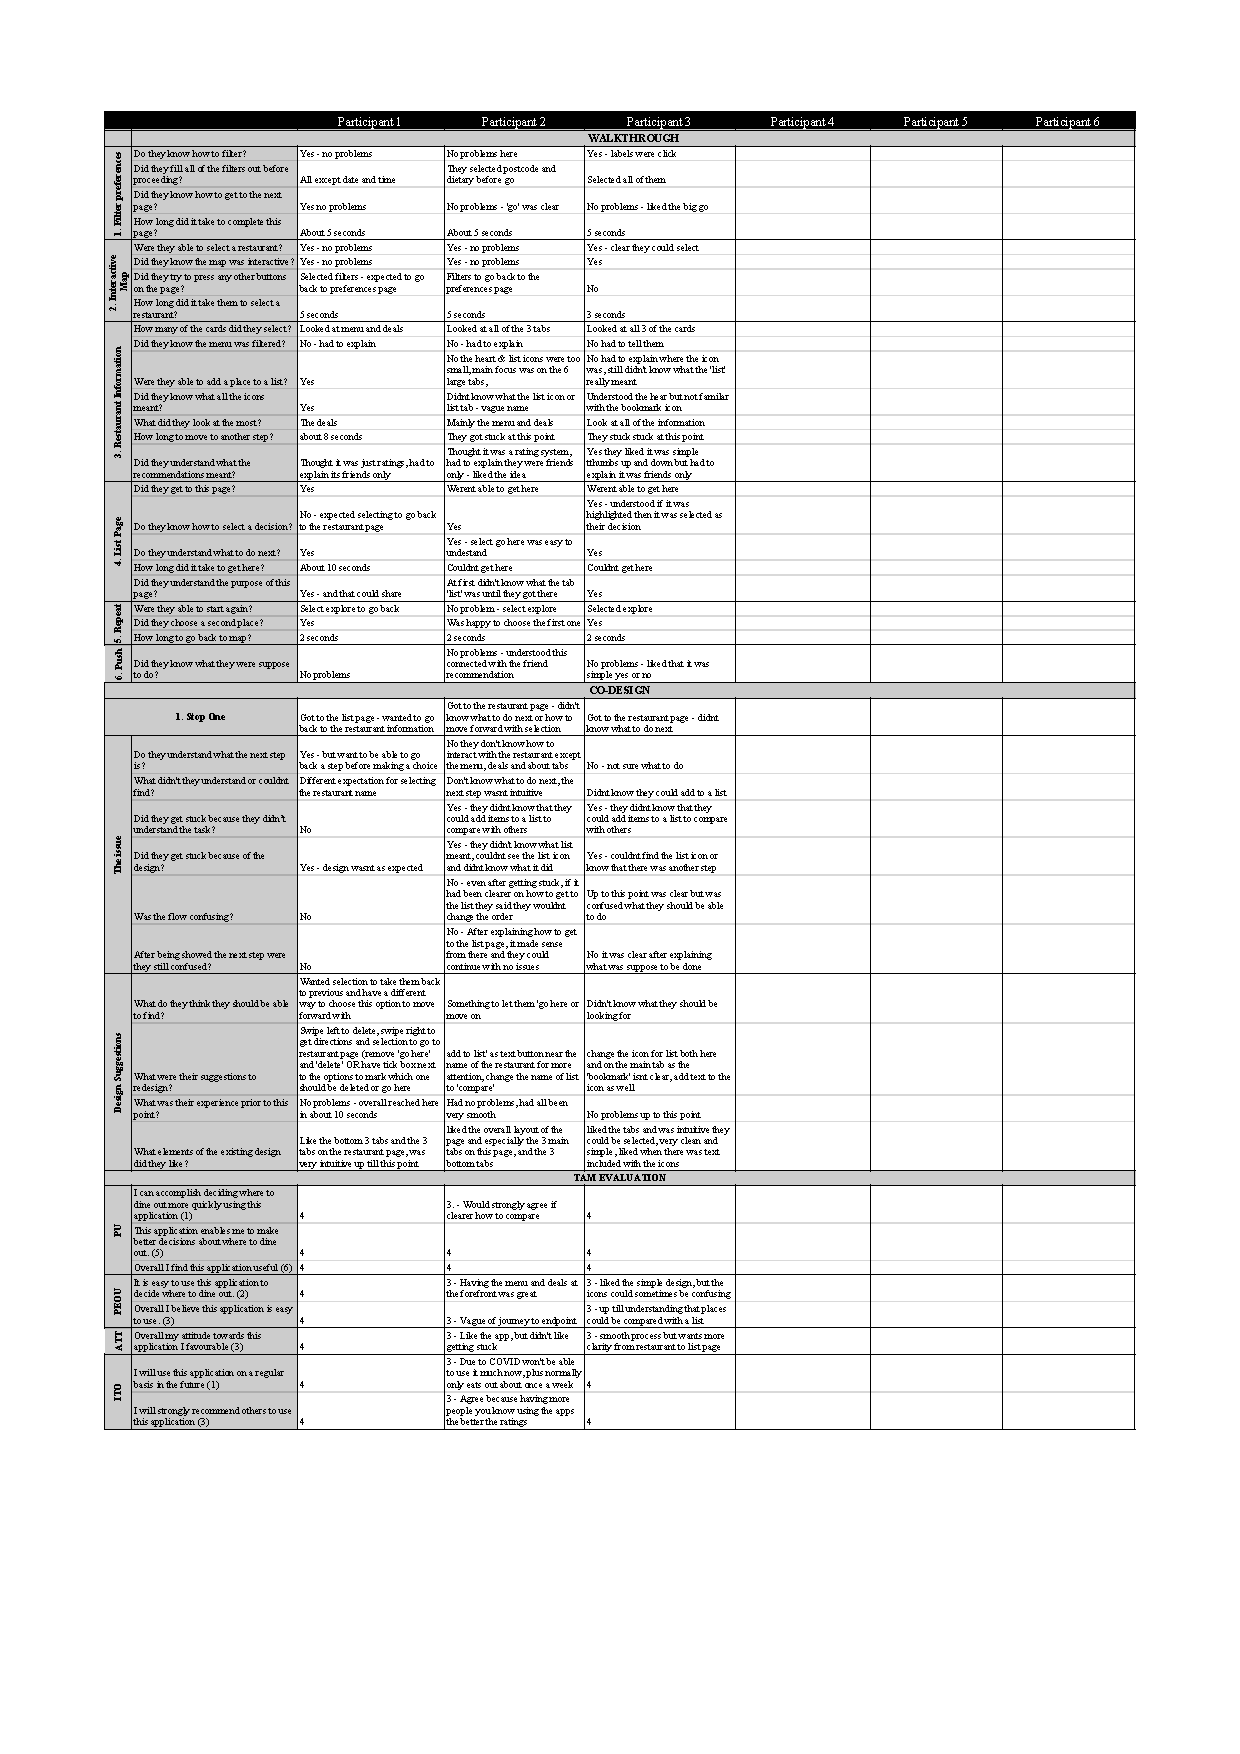
\includepdf[pages=-,pagecommand=\subsection{Interview Notes}, offset=0 -1.5cm]{Low_Fidelity/Low_Notes.pdf}
    \label{sec:A.5}


% MEDIUM FIDELITY 
% Title
\pagebreak
\begin{center}
    \vspace*{\stretch{0.7}}
    \Huge \textbf{Appendices}
    \section{Medium Fidelity Prototype}
    \vspace*{\stretch{1}}
\end{center}

    % Personas
    \pagebreak    
    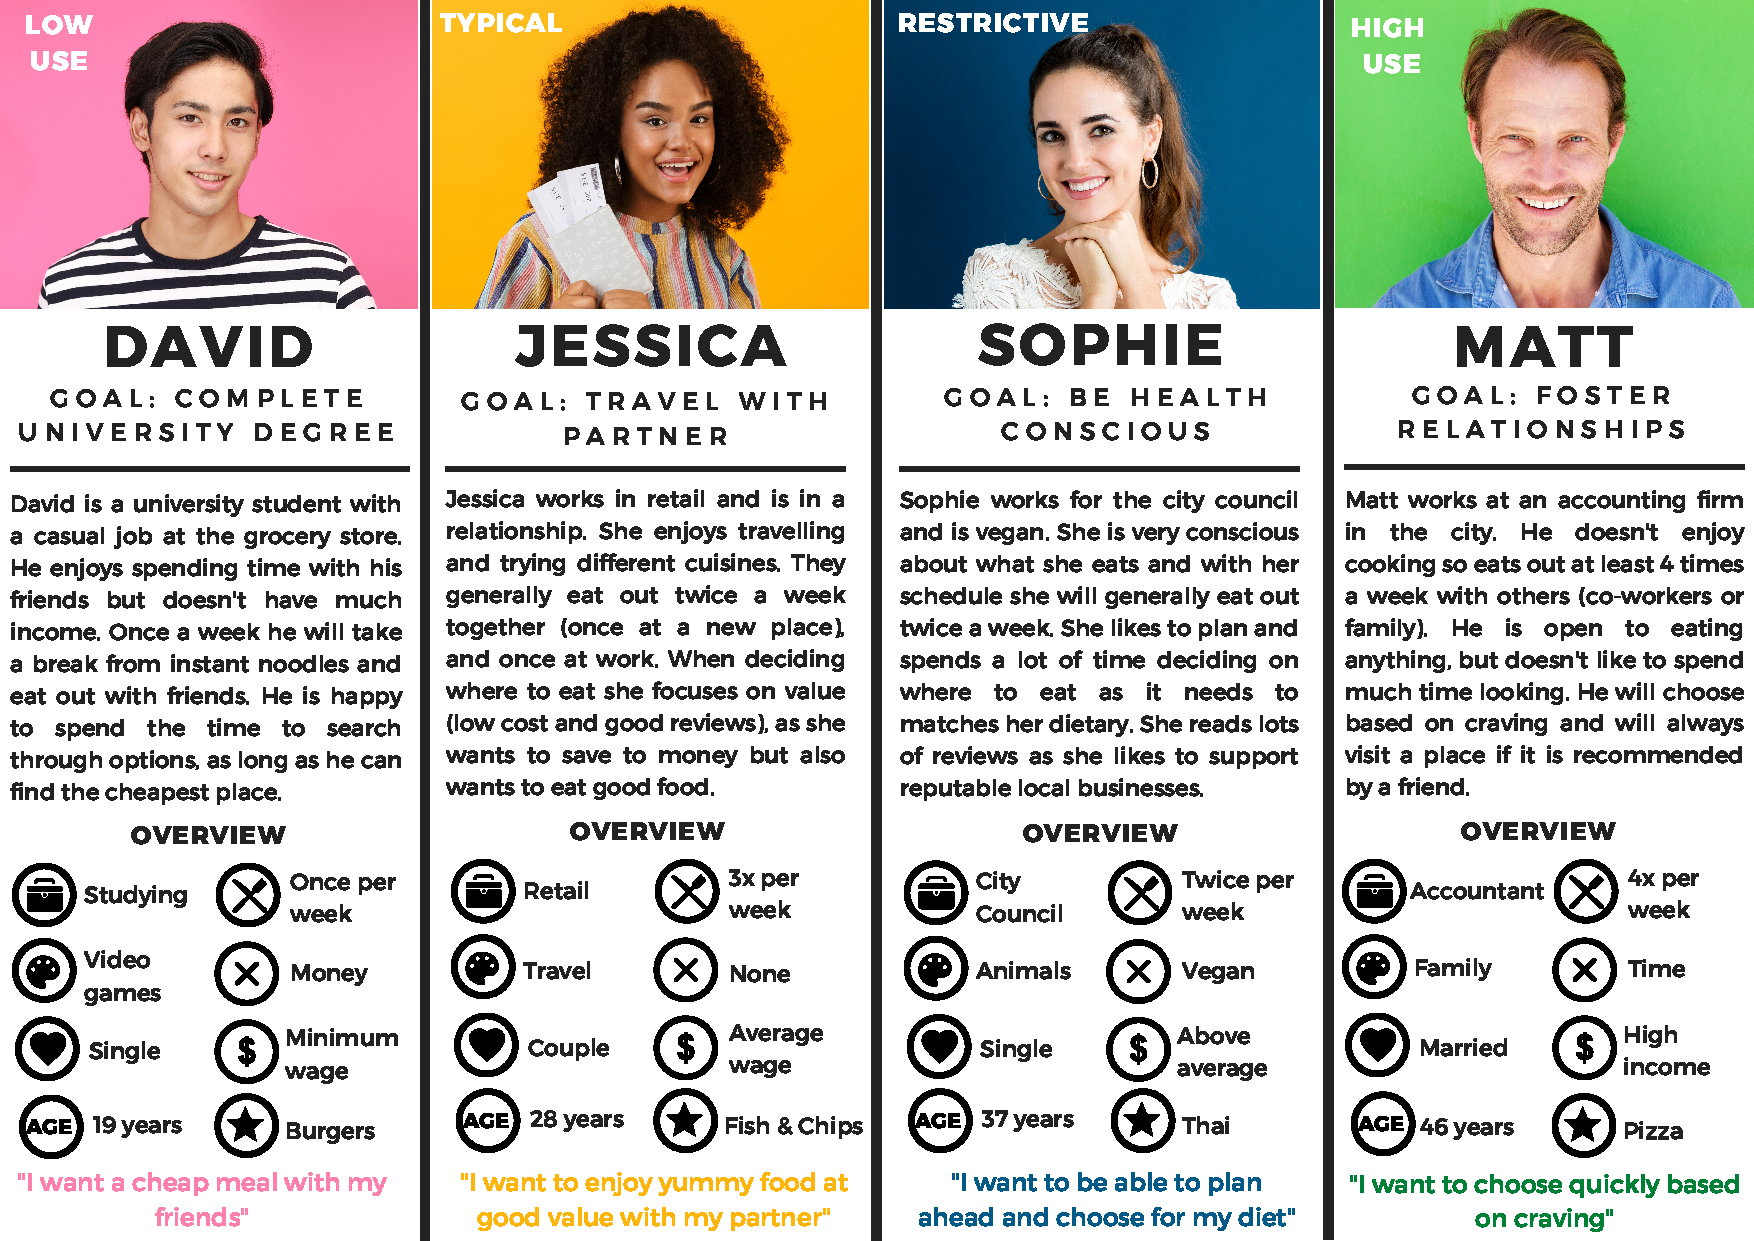
\includepdf[pages=-, 
                angle=90, 
                pagecommand=\subsection{Personas}, width=\textwidth,
                height=\textheight,
                keepaspectratio, 
                frame, offset= 0 -0.5cm]{Med_Fidelity/Personas.pdf}
                \label{sec:B.1}
    % Interaction Scenarios
    \pagebreak 
    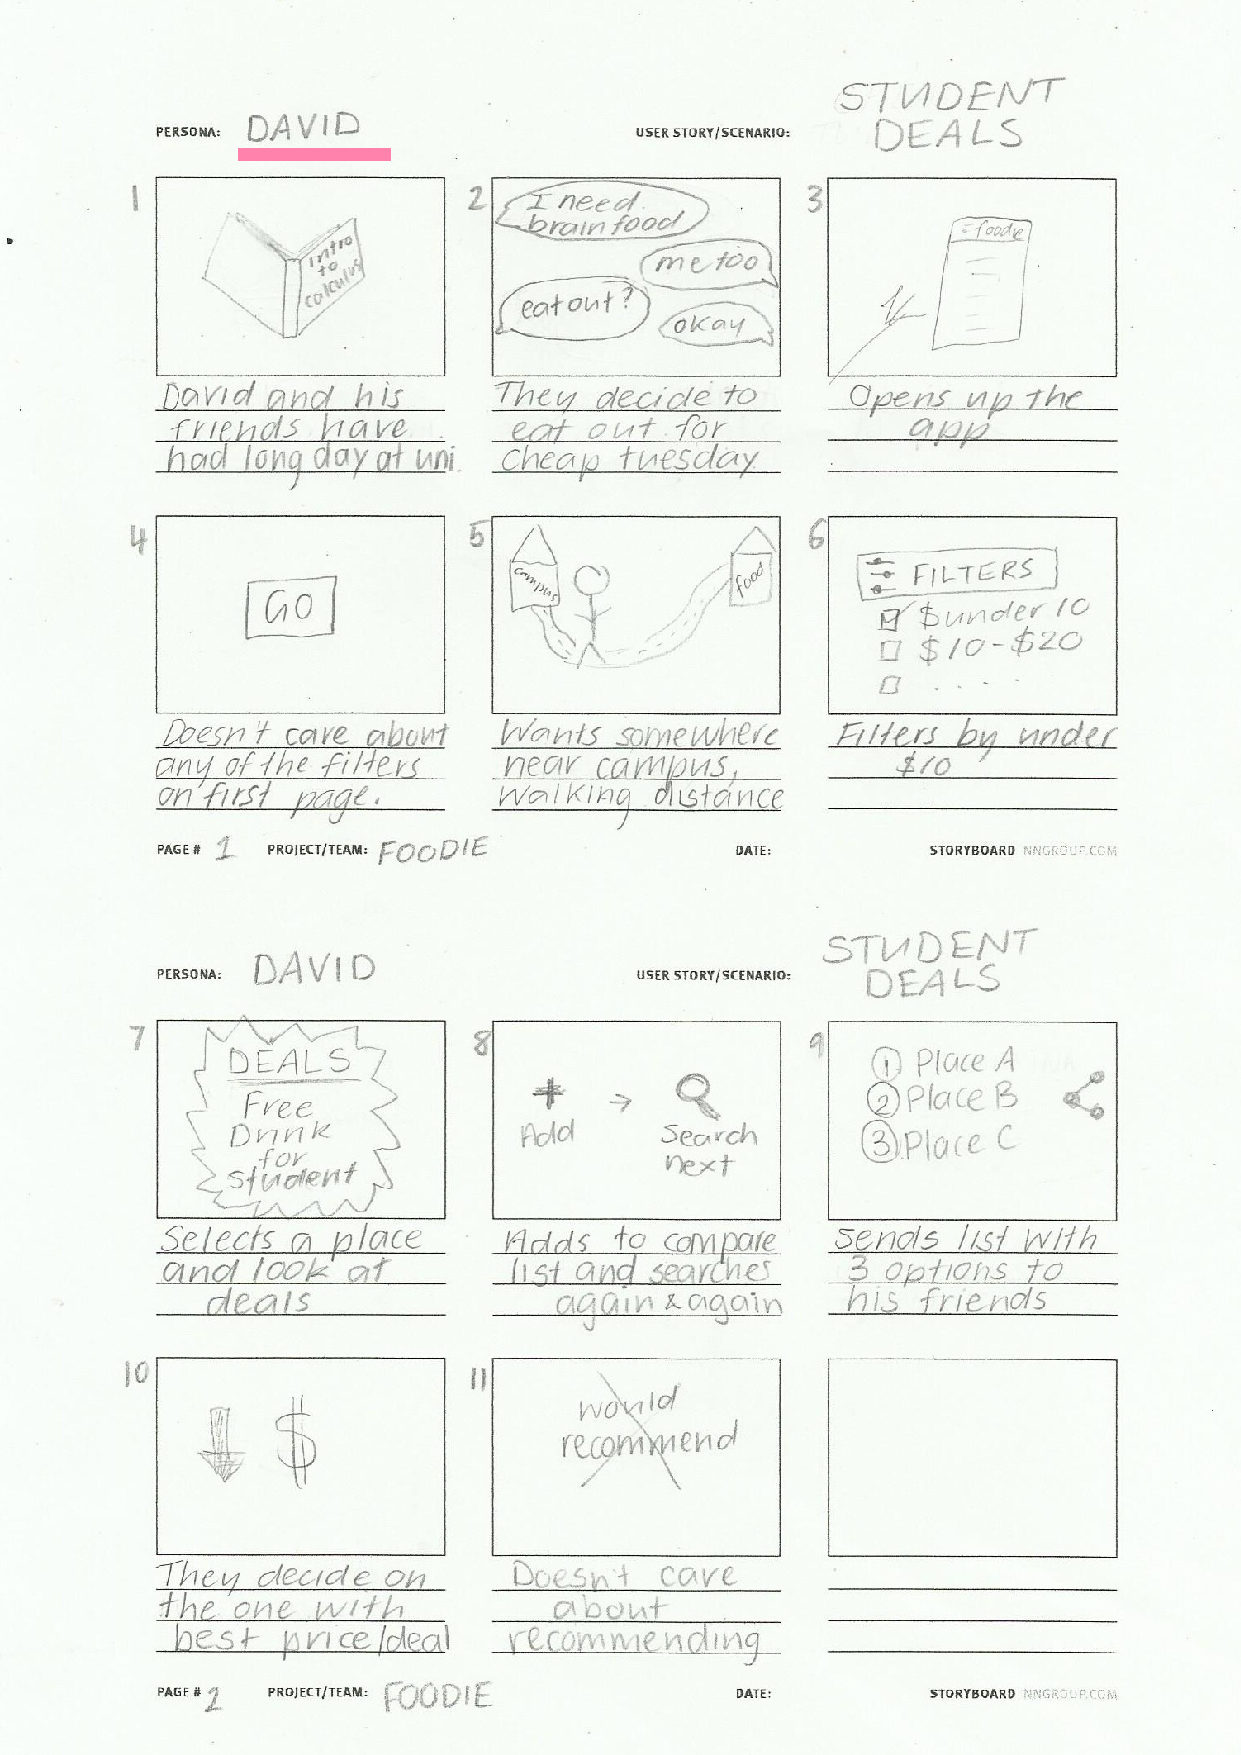
\includepdf[pages=1, 
                pagecommand=\subsection{Interaction Scenarios}, width=\textwidth,
                height=\textheight,
                keepaspectratio, 
                frame, offset= 0 -0.5cm]{Med_Fidelity/Scenarios.pdf}
                \label{sec:B.2} 
    \includepdf[pages=2-, 
                width=\textwidth,
                height=\textheight,
                keepaspectratio,
                frame, offset= 0 0cm]{Med_Fidelity/Scenarios.pdf}

    % UX Goals
    \pagebreak 
    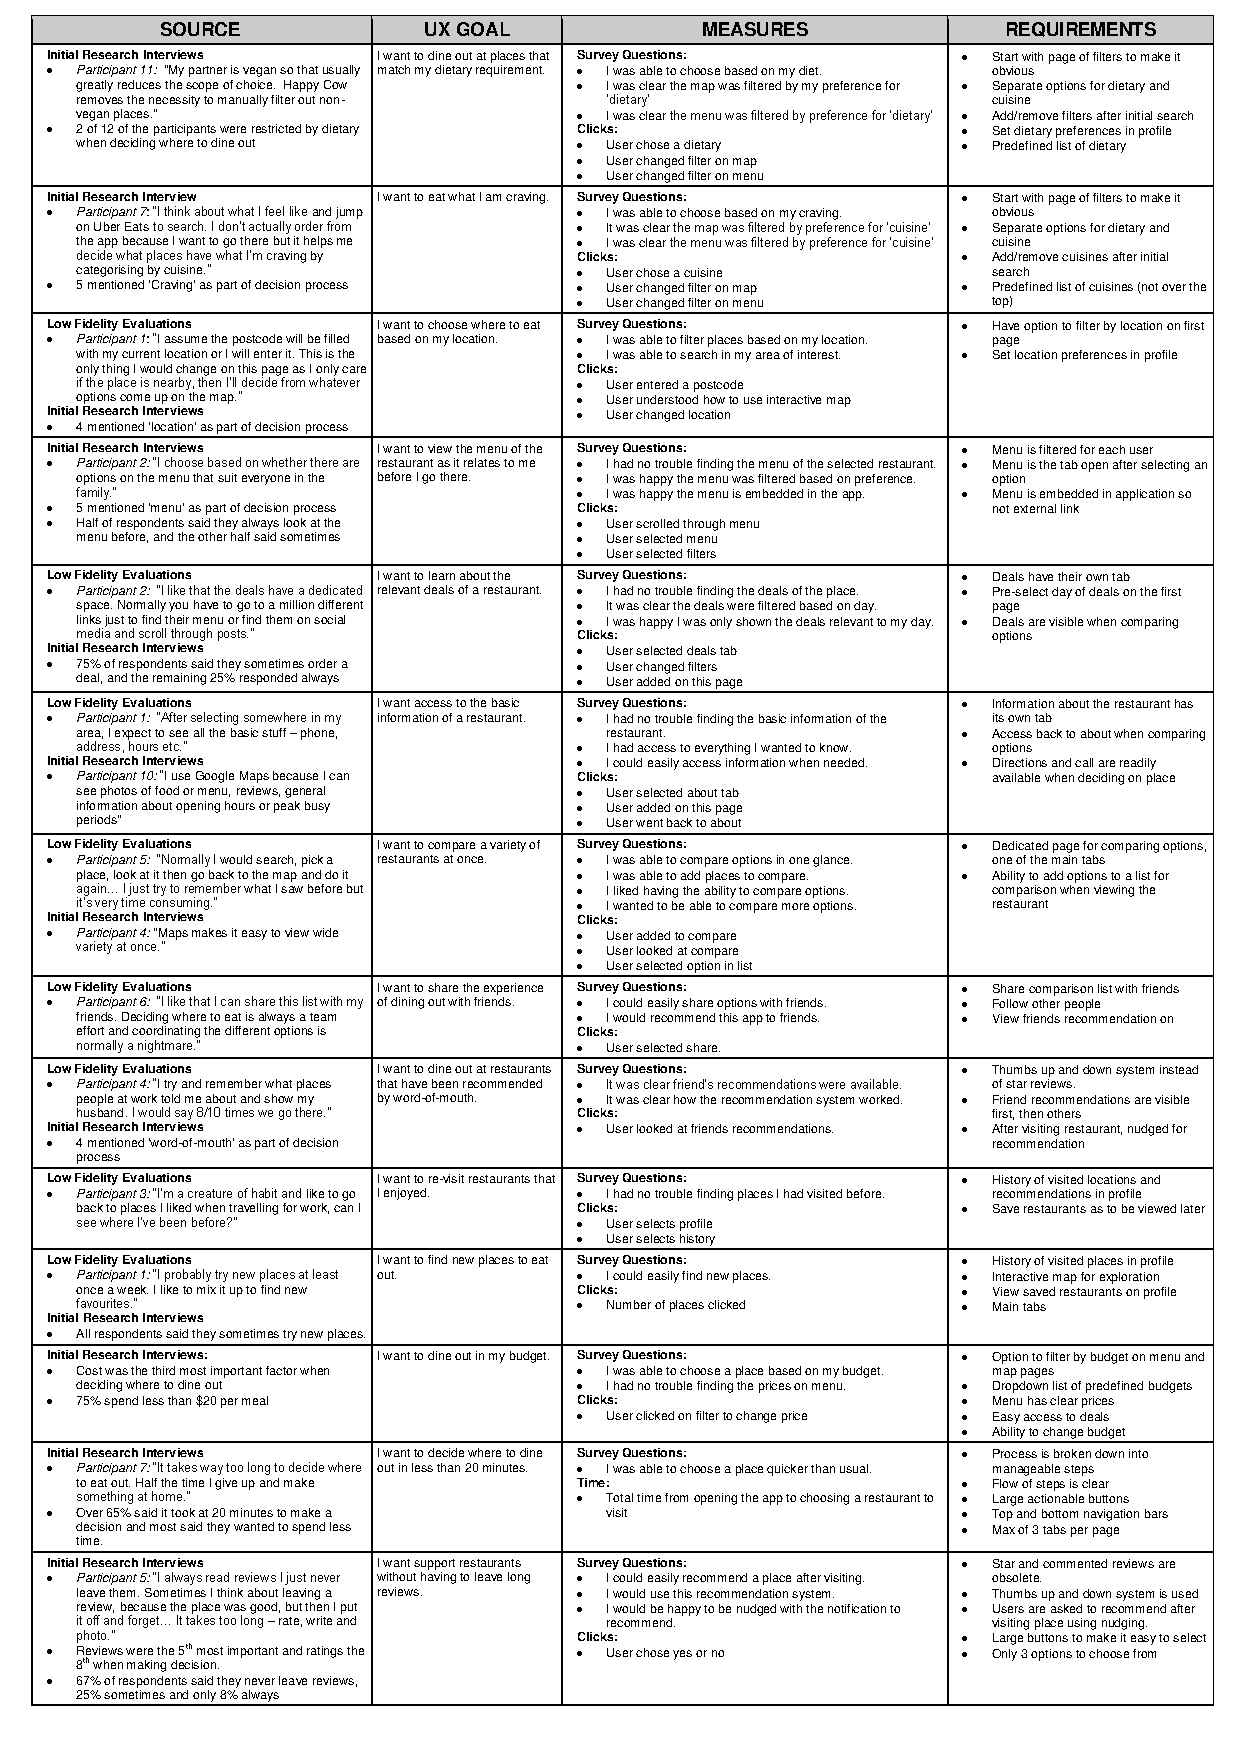
\includepdf[pages=1, 
                pagecommand=\subsection{UX Goals}, width=\textwidth,
                height=\textheight,
                keepaspectratio, 
                frame, offset= 0 -0.5cm]{Med_Fidelity/UX_Goals.pdf}                    
                \label{sec:B.3}

    % Evaluation Protocol
    \pagebreak     
    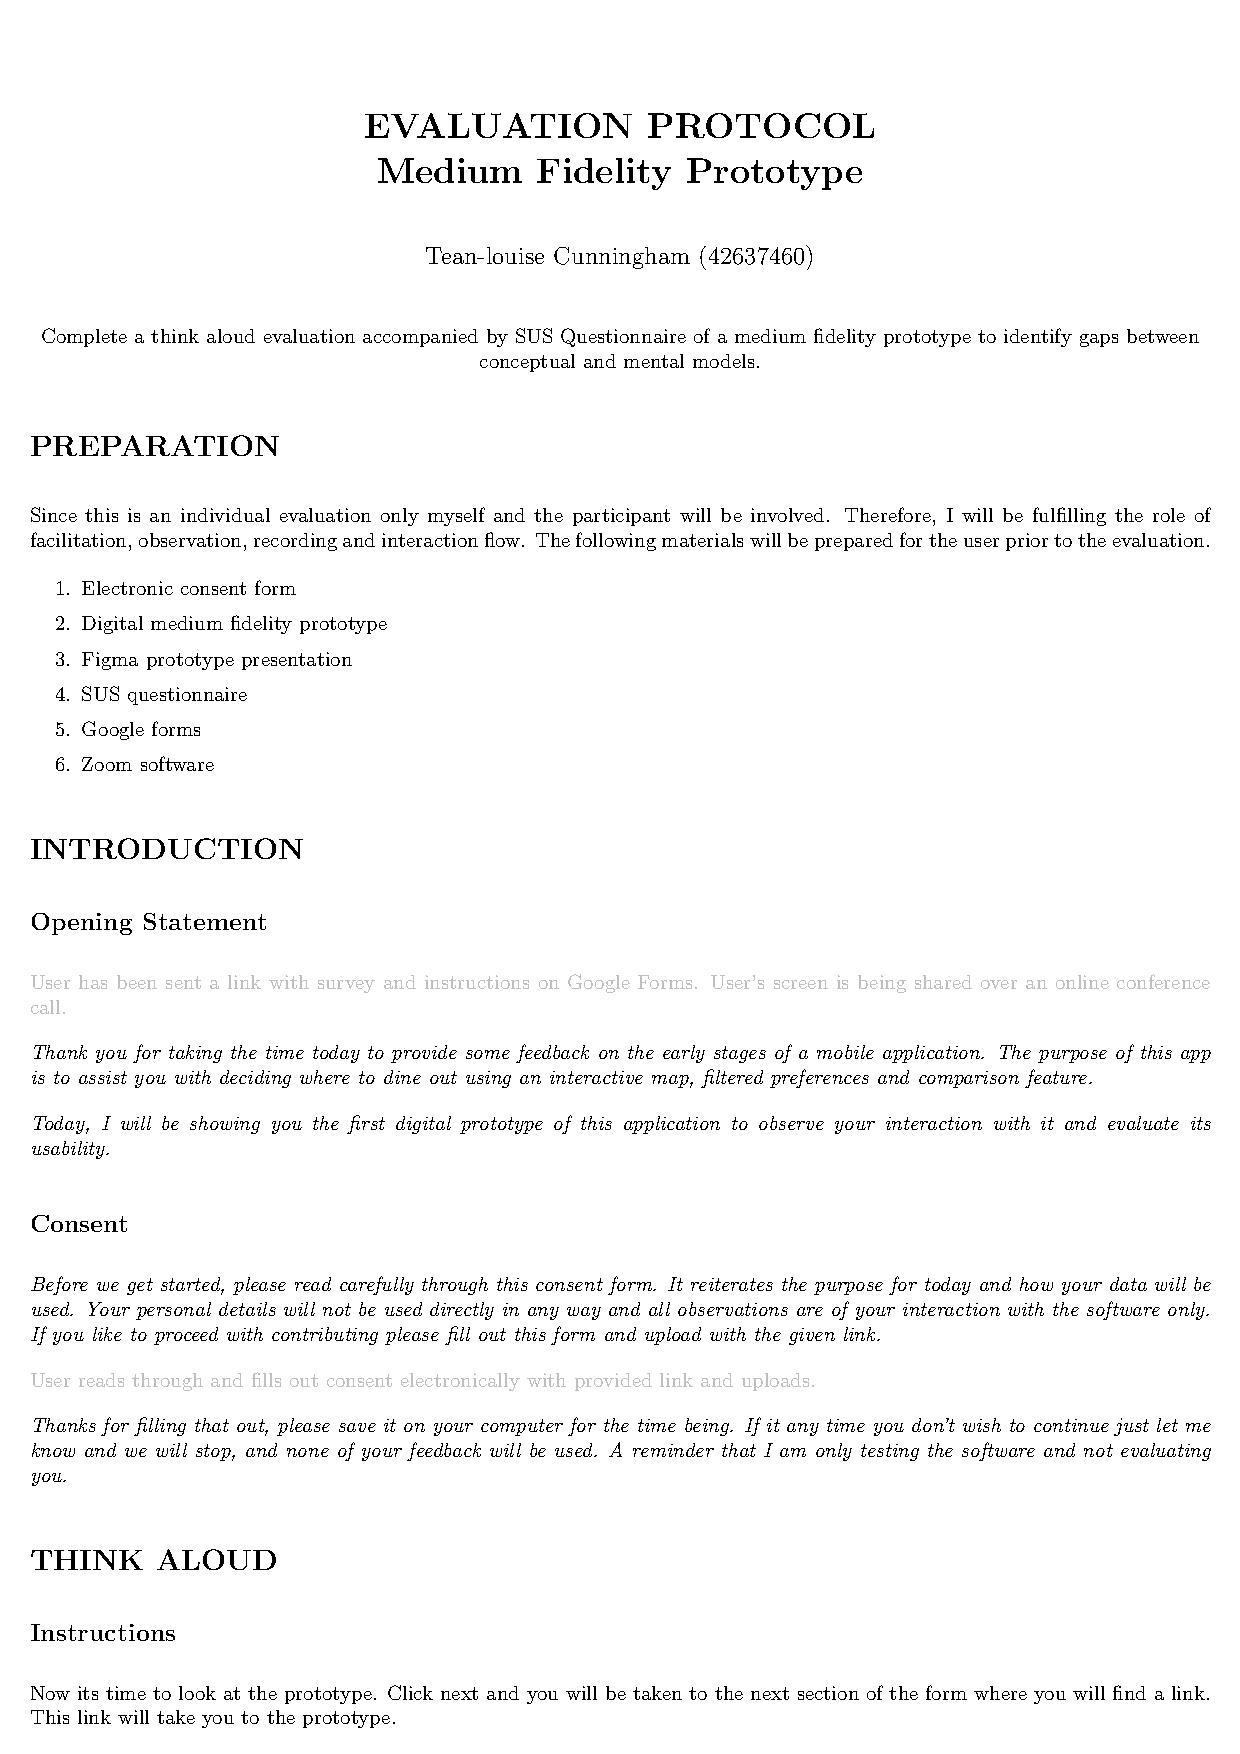
\includepdf[pages=1, 
                pagecommand=\subsection{Evaluation Protocol}, 
                width=\textwidth,
                height=\textheight,
                keepaspectratio, 
                frame, offset= 0 -0.5cm]
                    {Med_Fidelity/Med_Protocol/Med_Protocol.pdf}
                    \label{sec:B.4}
    \includepdf[pages=2-, 
                width=\textwidth,
                height=\textheight,
                keepaspectratio,
                frame, offset= 0 0cm]
                    {Med_Fidelity/Med_Protocol/Med_Protocol.pdf}

    % Google Forms
    \pagebreak     
    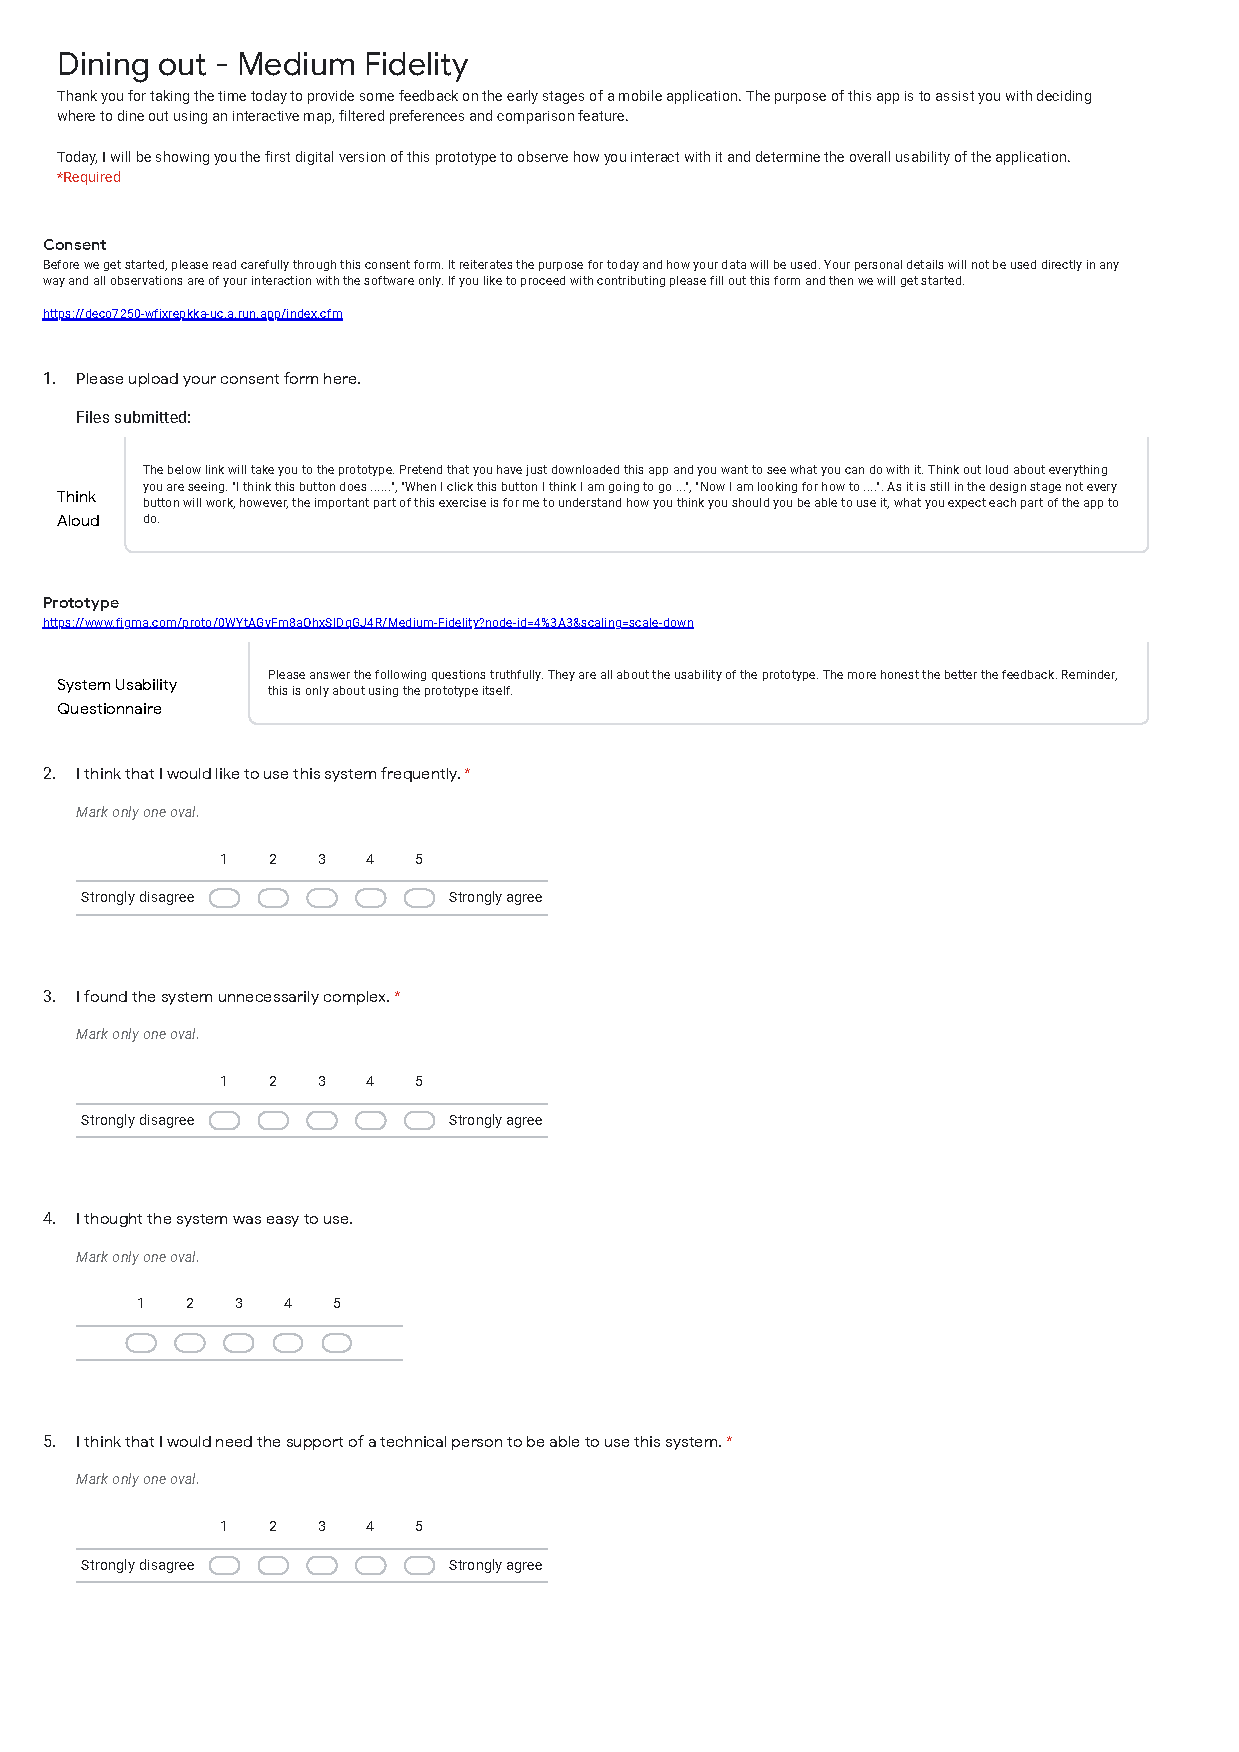
\includepdf[pages=1, 
                pagecommand=\subsection{Evaluation - Google Forms}, 
                width=\textwidth,
                height=\textheight,
                keepaspectratio, 
                frame, offset= 0 -0.5cm]{Med_Fidelity/Med_Form.pdf}
                \label{sec:B.5}
    \includepdf[pages=2-, 
                width=\textwidth,
                height=\textheight,
                keepaspectratio,
                frame, offset= 0 0cm]{Med_Fidelity/Med_Form.pdf}

    % Presentation
    \pagebreak     
    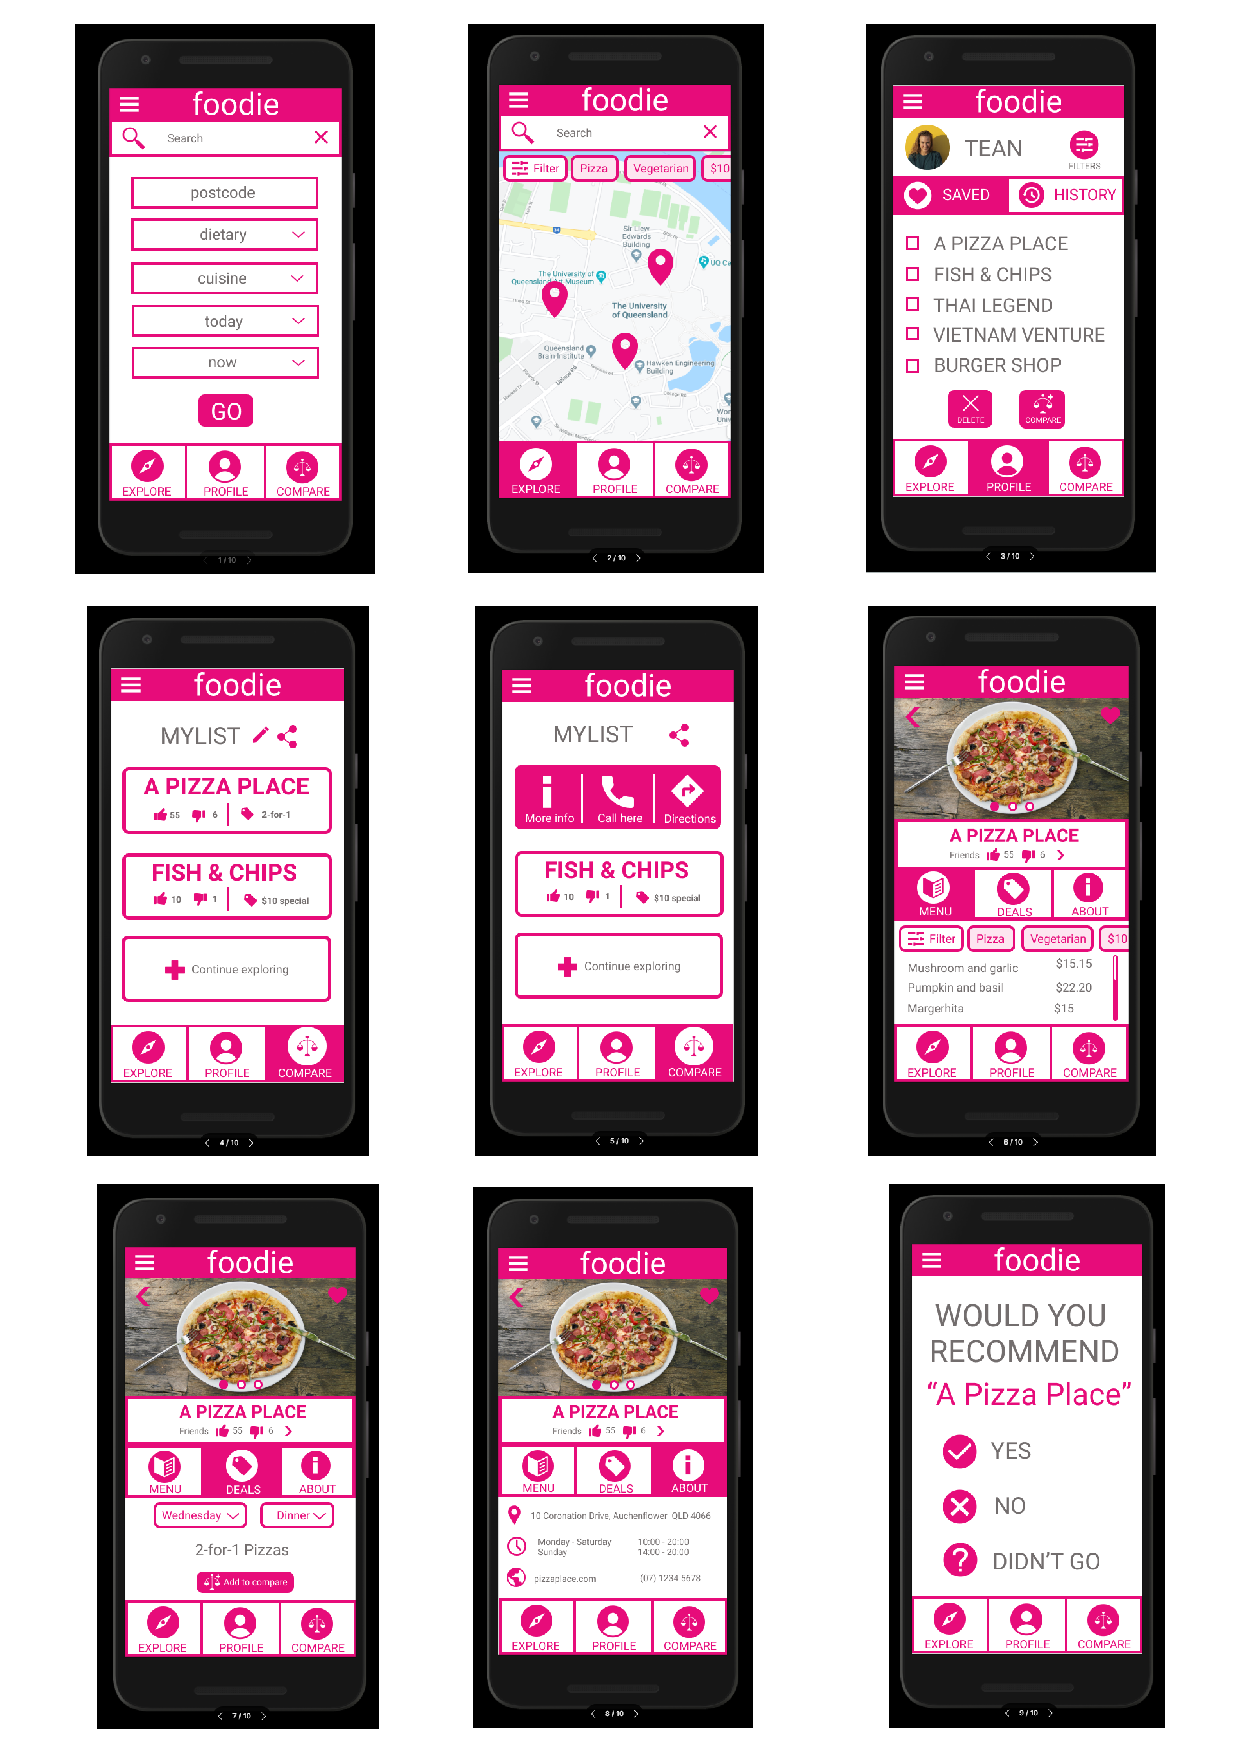
\includepdf[pages=1, 
                pagecommand=\subsection{Evaluation - Presentation}, 
                width=\textwidth,
                height=\textheight,
                keepaspectratio, 
                frame, offset= 0 -0.5cm]{Med_Fidelity/Med_Slides.pdf}
                \label{sec:B.6}


    % Questionnaire Results
    \pagebreak    
    \subsection{Evaluation - SUS Results}
    \label{sec:B.7} 

    \subsubsection*{Raw Data}
        \begin{figure} [H]
            \centering
            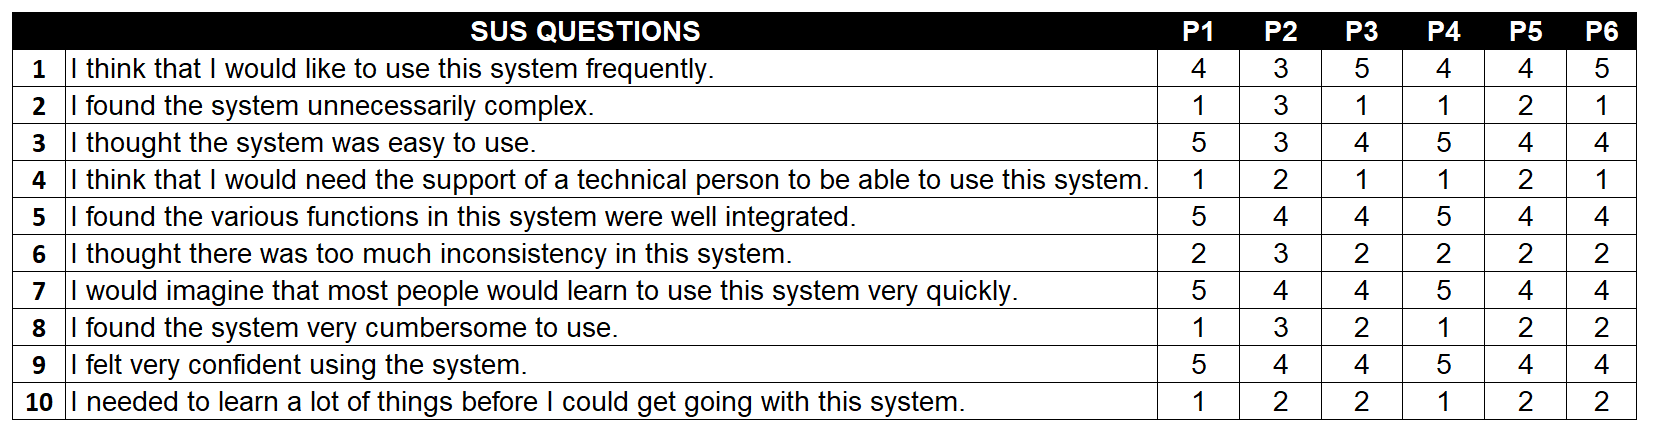
\includegraphics[width=0.9\textwidth, frame]
                {./Med_Fidelity/Med_SUS_Raw.PNG}  
            \caption{SUS Raw Data}
        \end{figure}

    \subsubsection*{SUS Scores (Steps 1-3)}
        \begin{figure} [H]
            \centering
            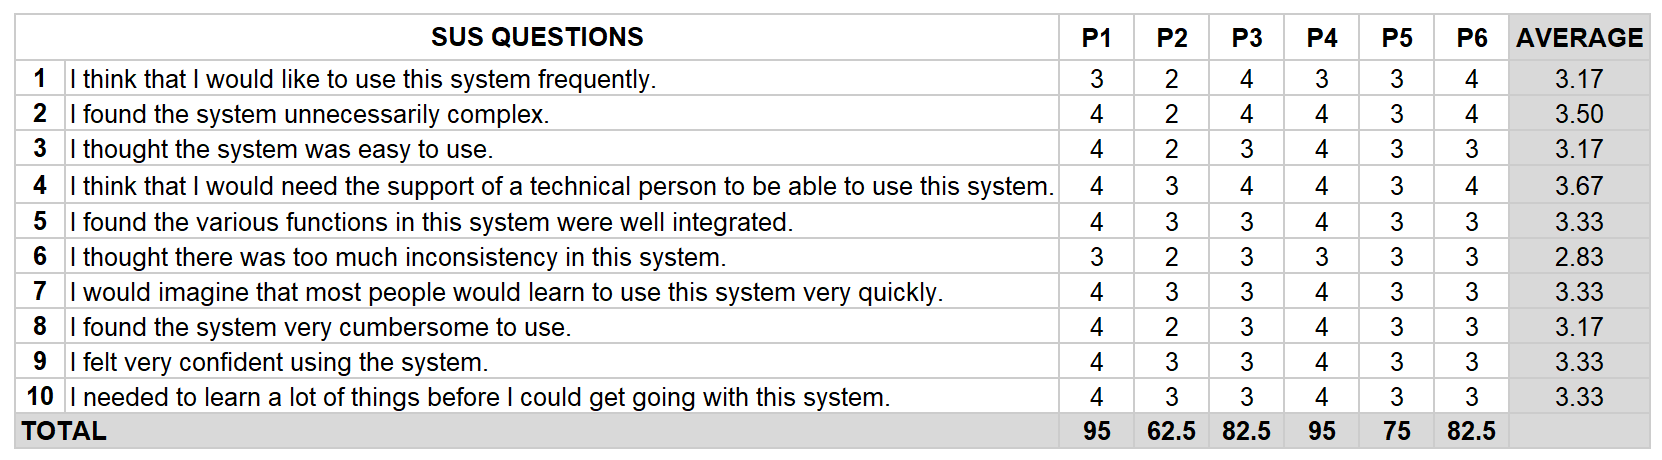
\includegraphics[width=0.9\textwidth, frame]
                {./Med_Fidelity/Med_SUS_Scores.PNG}  
            \caption{SUS Scores}
        \end{figure}
    
    \subsubsection*{SUS Distribution (Step 4)}
        \begin{figure} [H]
            \centering
            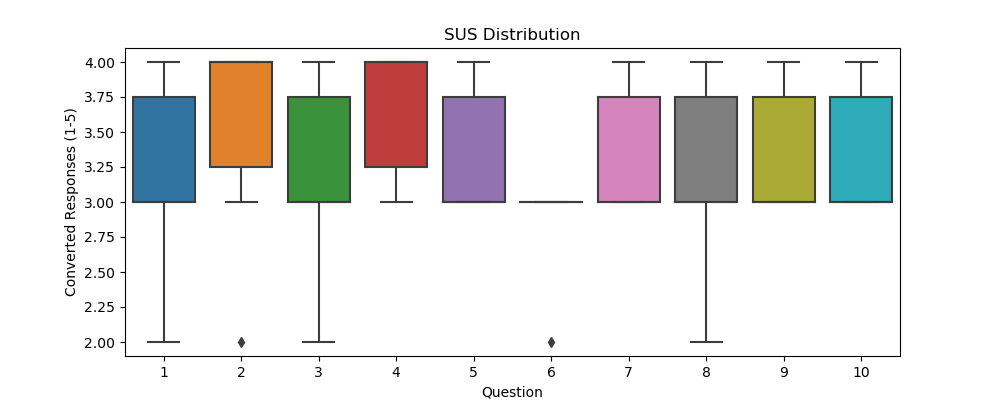
\includegraphics[width=0.9\textwidth, frame]
                {./Med_Fidelity/Med_SUS_Distrib.PNG}  
            \caption{SUS Distribution}
        \end{figure}

    % Notes

    \pagebreak     
    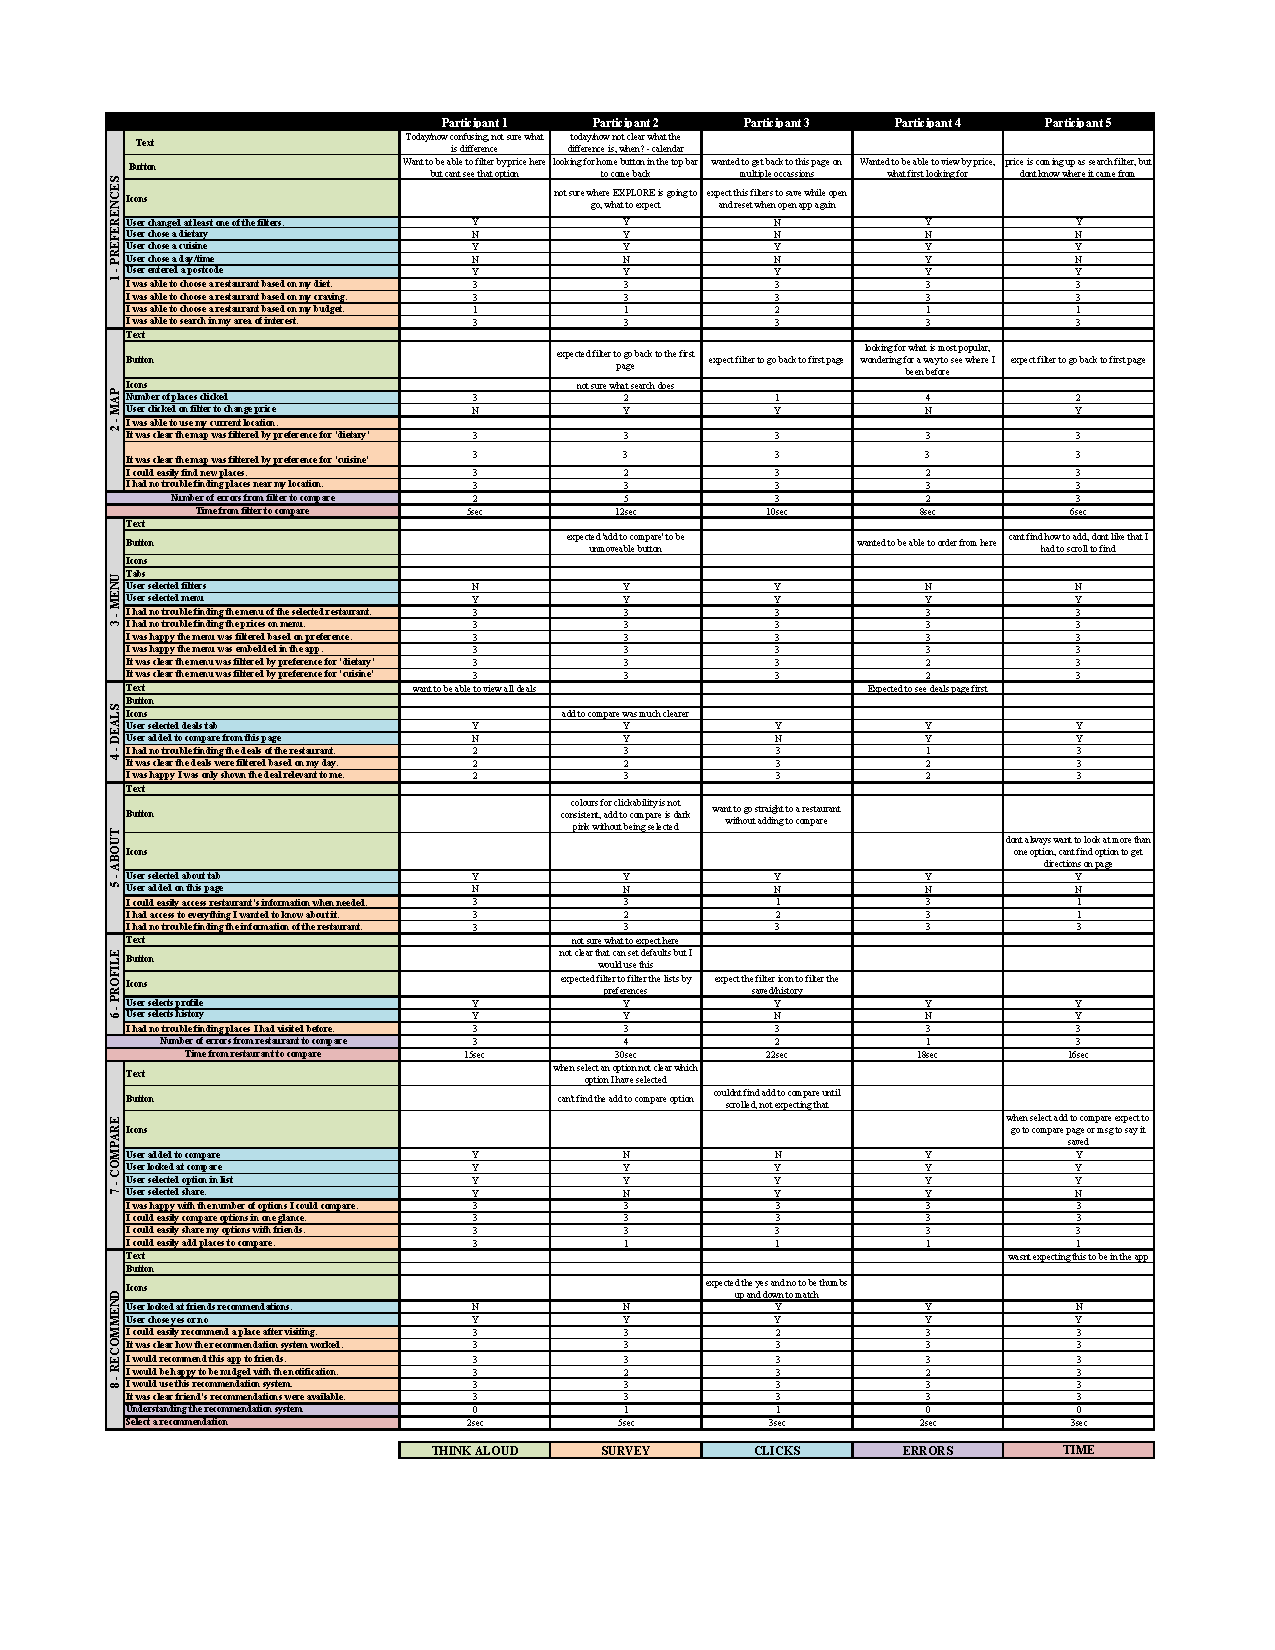
\includepdf[pages=-, 
                pagecommand=\subsection{Evaluation - Notes}, 
                %width=\textwidth,
                %height=\textheight,
                keepaspectratio, 
                offset= 0 0cm]{Med_Fidelity/Med_Notes.pdf}
                \label{sec:B.8}

% HIGH FIDELITY 
% Title
\pagebreak
\begin{center}
    \vspace*{\stretch{0.7}}
    \Huge \textbf{Appendices}
    \section{High Fidelity Prototype}
    \vspace*{\stretch{1}}
\end{center}


    % Evaluation Protocol
    \pagebreak     
    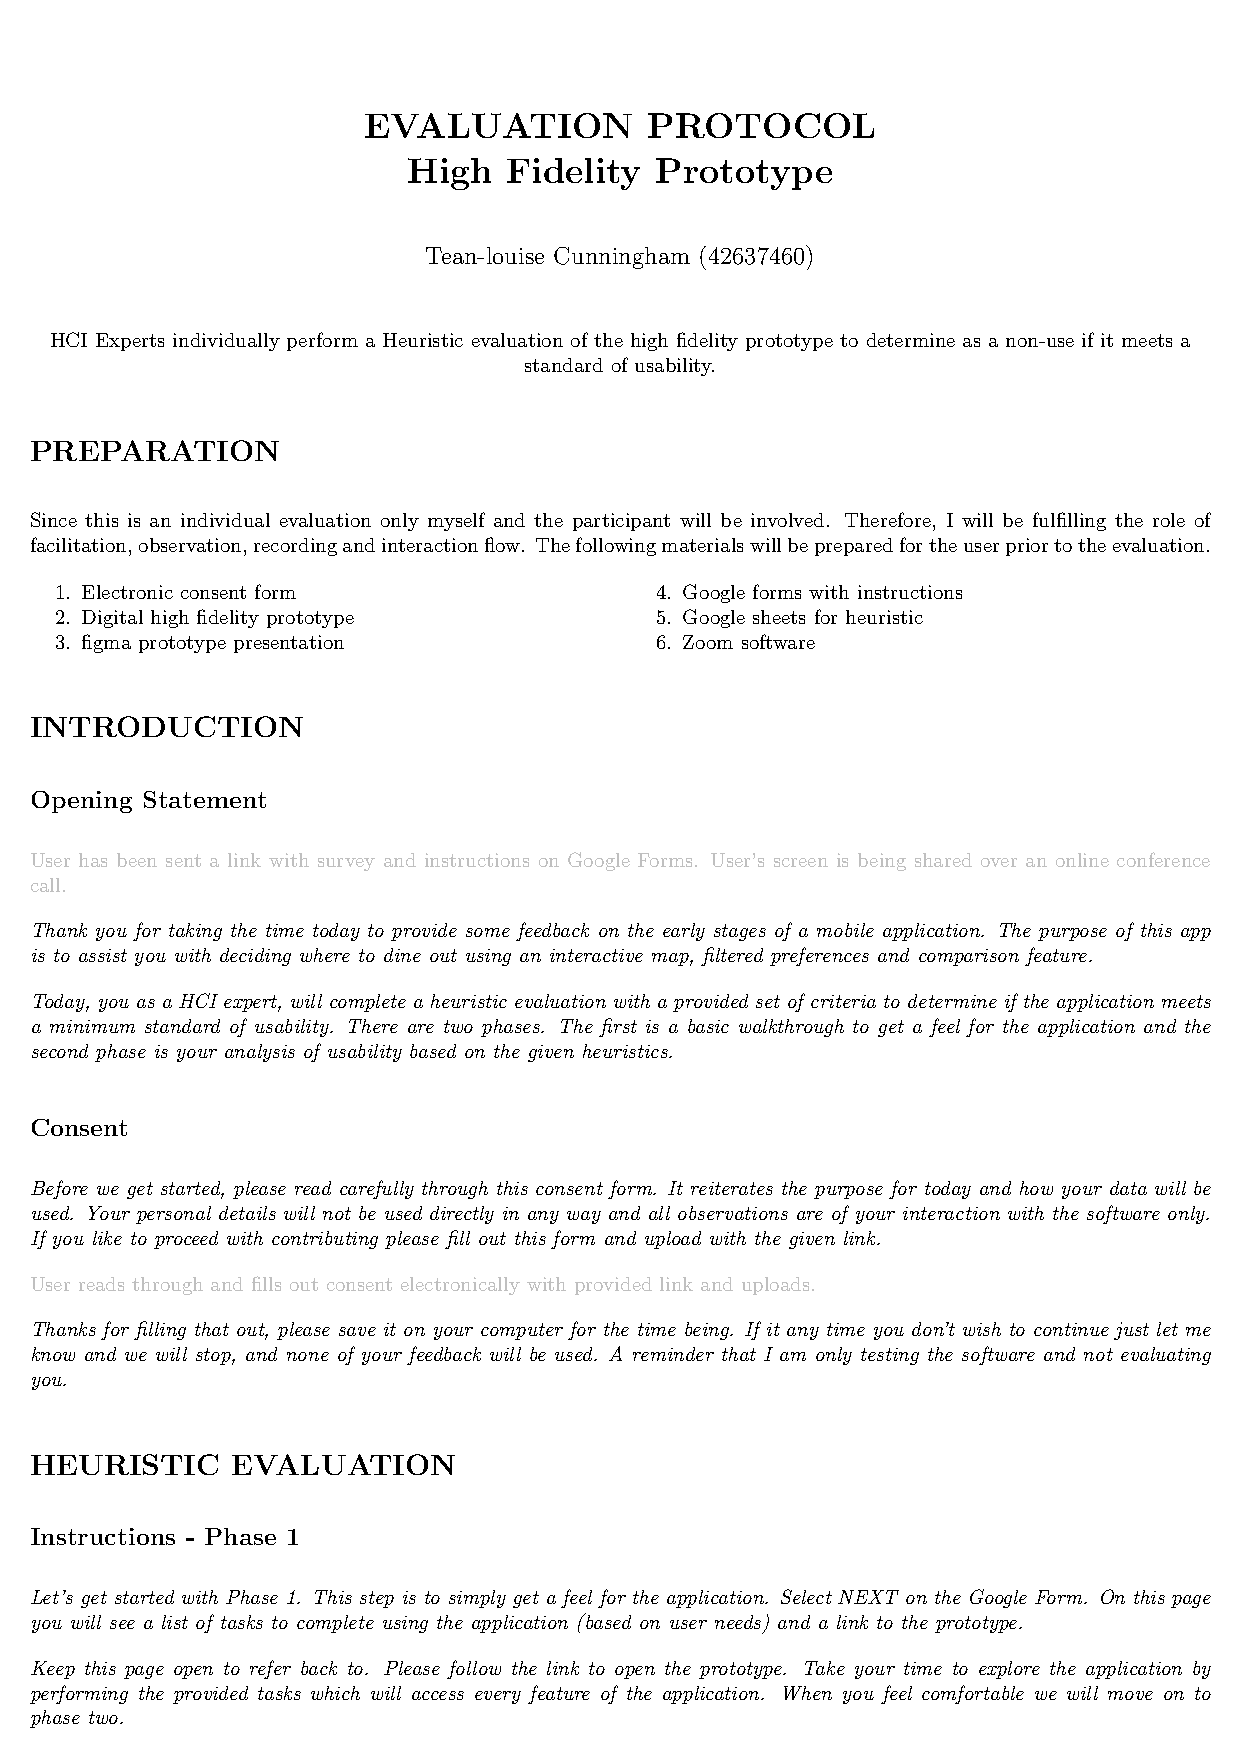
\includepdf[pages=1, 
                pagecommand=\subsection{Evaluation Protocol}, 
                width=\textwidth,
                height=\textheight,
                keepaspectratio, 
                frame, offset= 0 -0.5cm]
                    {High_Fidelity/High_Protocol/High_Protocol.pdf}
                    \label{sec:C.1}
    \includepdf[pages=2-, 
                width=\textwidth,
                height=\textheight,
                keepaspectratio,
                frame, offset= 0 0cm]
                    {High_Fidelity/High_Protocol/High_Protocol.pdf}

    % Google Forms
    \pagebreak     
    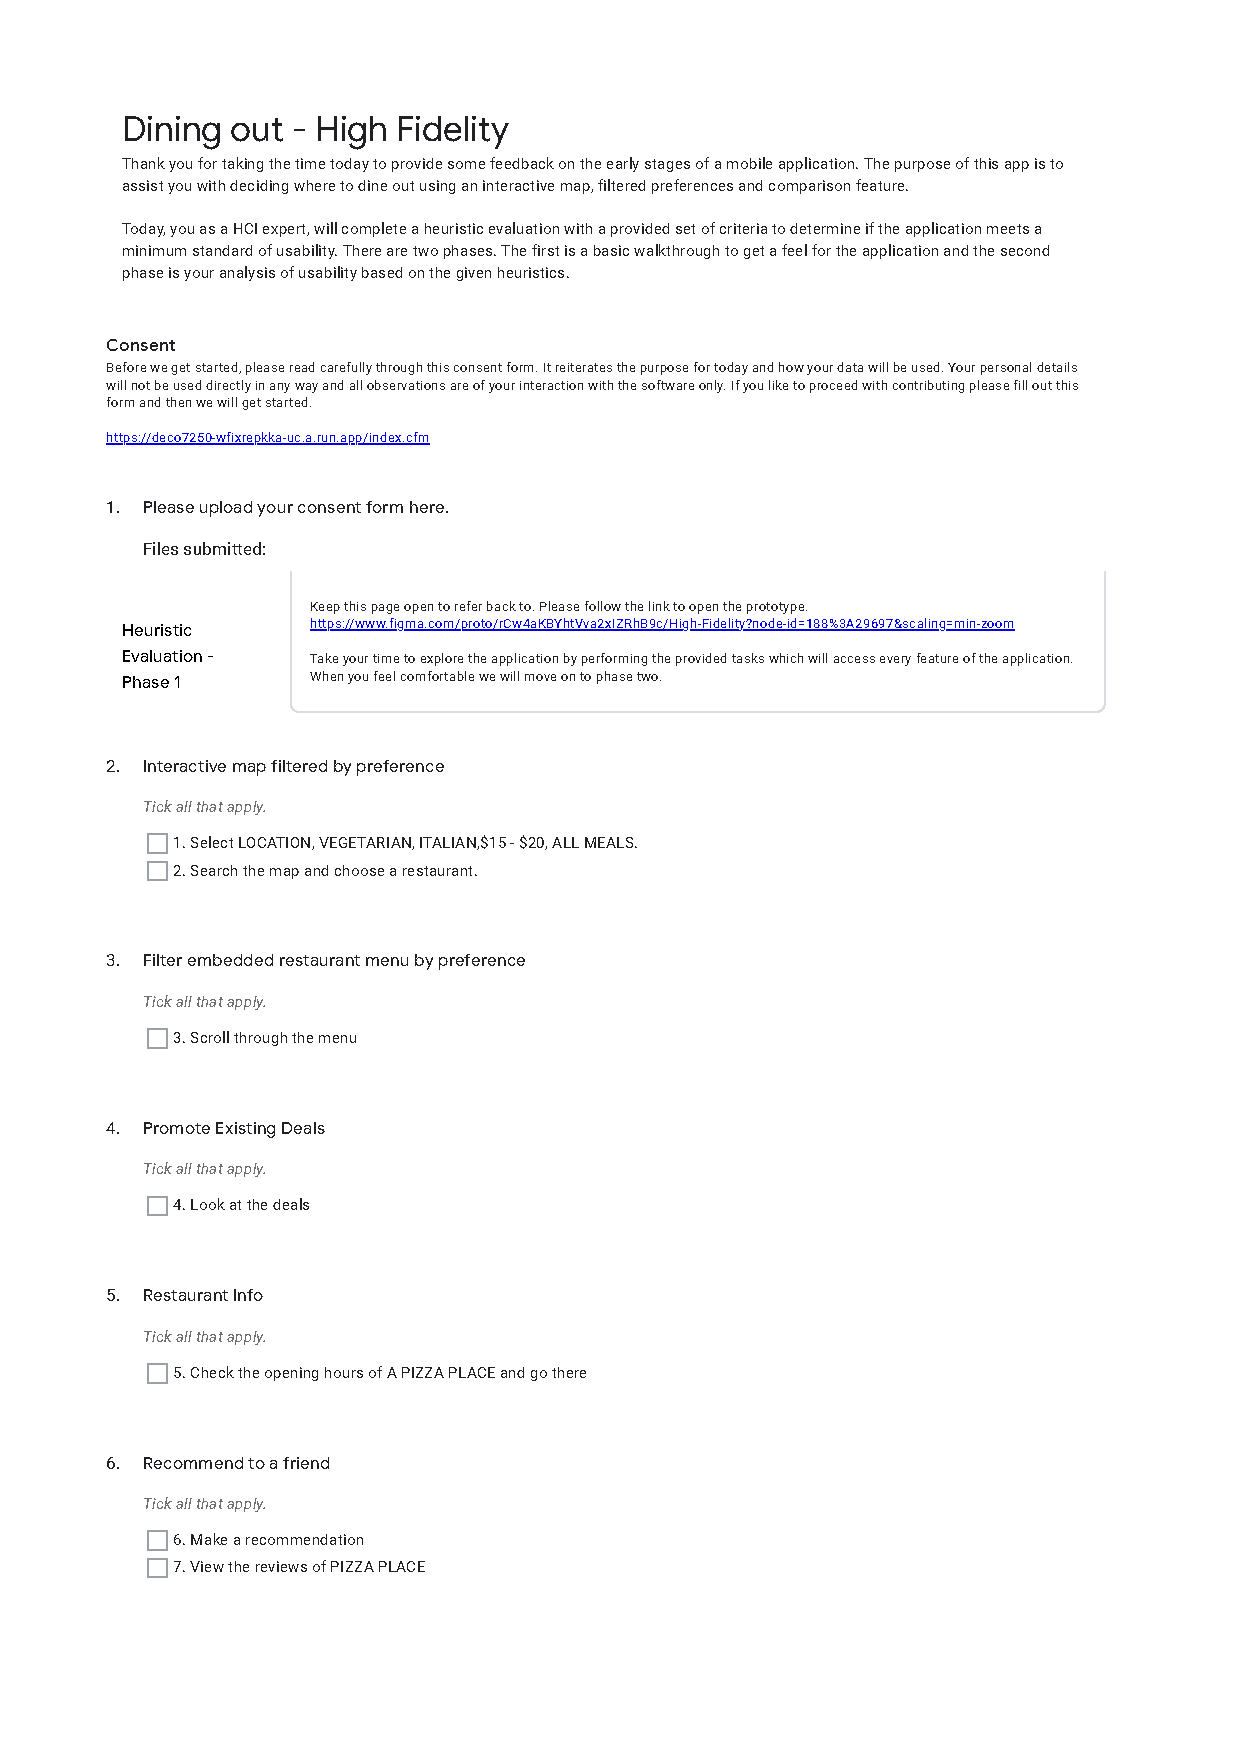
\includepdf[pages=1, 
                pagecommand=\subsection{Evaluation - Google Forms}, 
                width=\textwidth,
                height=\textheight,
                keepaspectratio, 
                frame, offset= 0 -0.5cm]{High_Fidelity/High_Form.pdf}
                \label{sec:C.2}
    \includepdf[pages=2-, 
                width=\textwidth,
                height=\textheight,
                keepaspectratio,
                frame, offset= 0 0cm]{High_Fidelity/High_Form.pdf}

    % Presentation
    \pagebreak     
    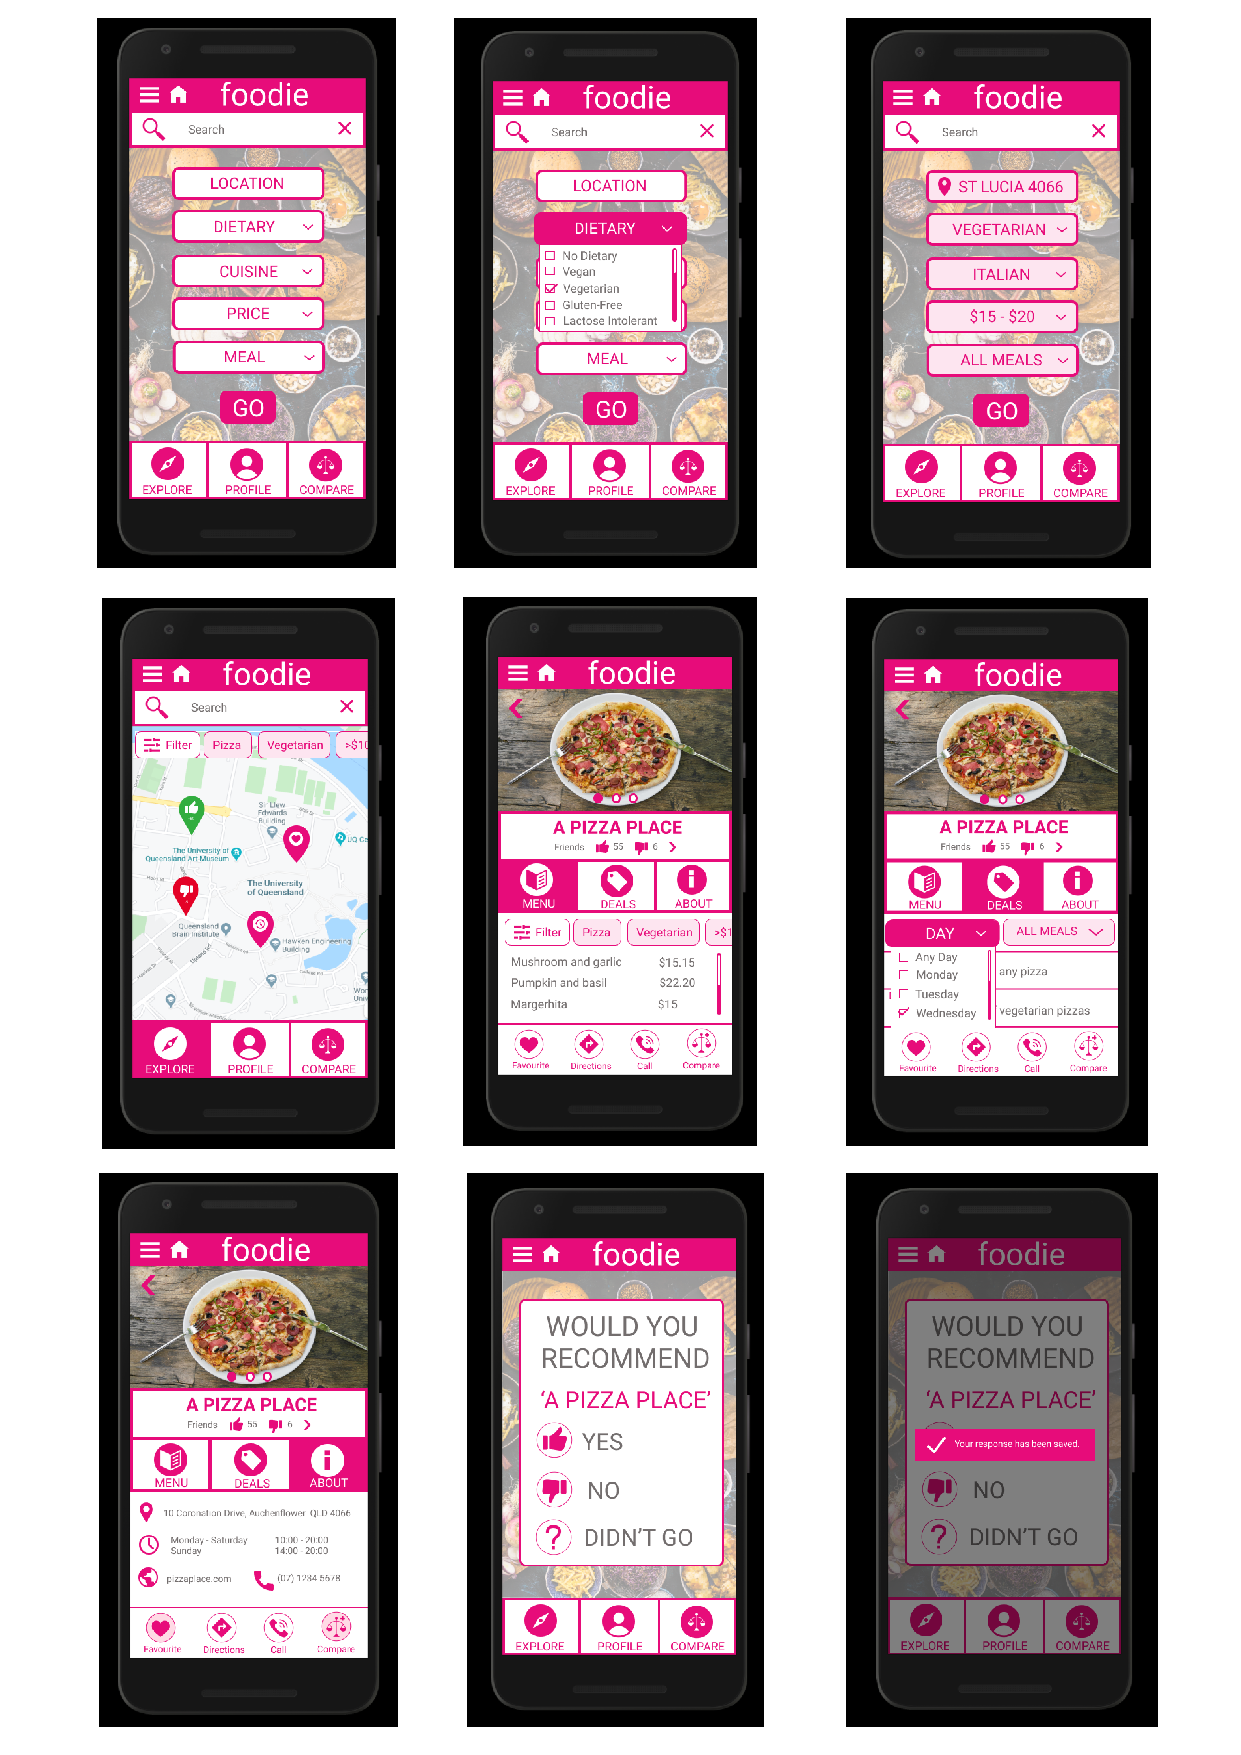
\includepdf[pages=1, 
                pagecommand=\subsection{Evaluation - Presentation}, 
                width=\textwidth,
                height=\textheight,
                keepaspectratio, 
                frame, offset= 0 -0.5cm]{High_Fidelity/High_Slides.pdf}
                \label{sec:C.3}
    \includepdf[pages=2, 
                width=\textwidth,
                height=\textheight,
                keepaspectratio,
                frame, offset= 0 0cm]{High_Fidelity/High_Slides.pdf}

    % Google Sheets
    \pagebreak  
    \subsection{Evaluation - Notes Template}
    \label{sec:C.4} 

    \subsubsection*{Heuristics (Tab 1)}
    \begin{figure} [H]
        \centering
        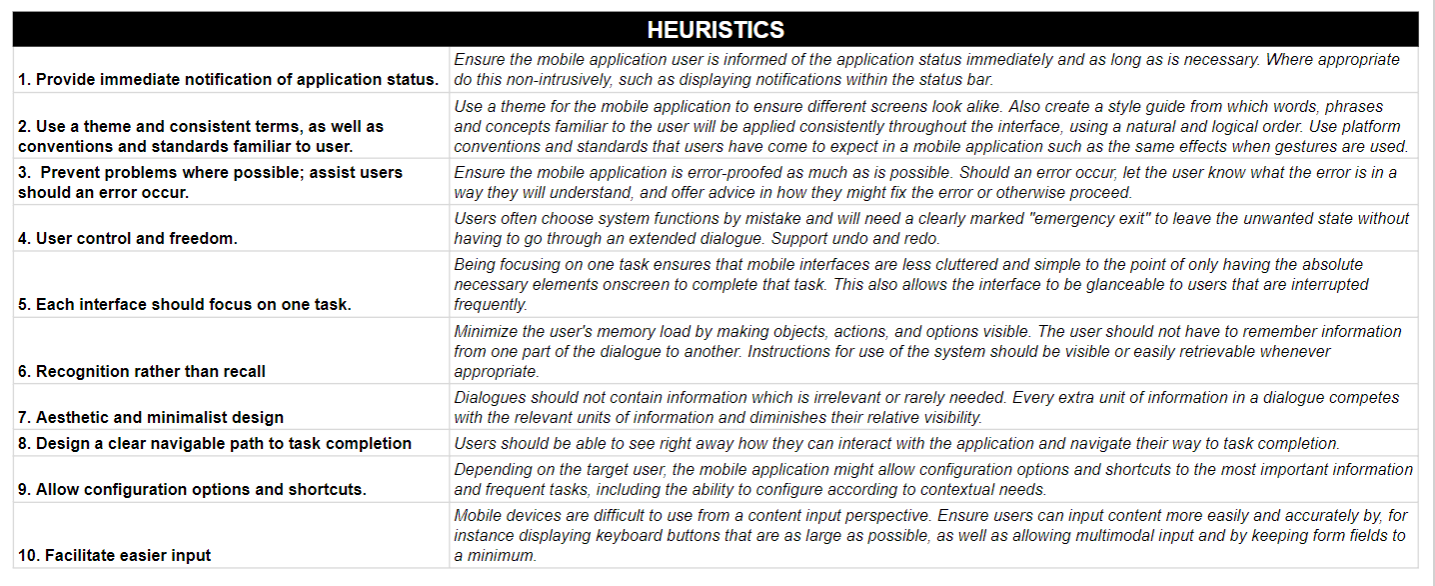
\includegraphics[width=0.9\textwidth, frame]
            {./High_Fidelity/High_Heuristics.PNG}
    \end{figure}

    \subsubsection*{Expert Notes Template (Tab 2)}

    \begin{figure} [H]
        \centering
        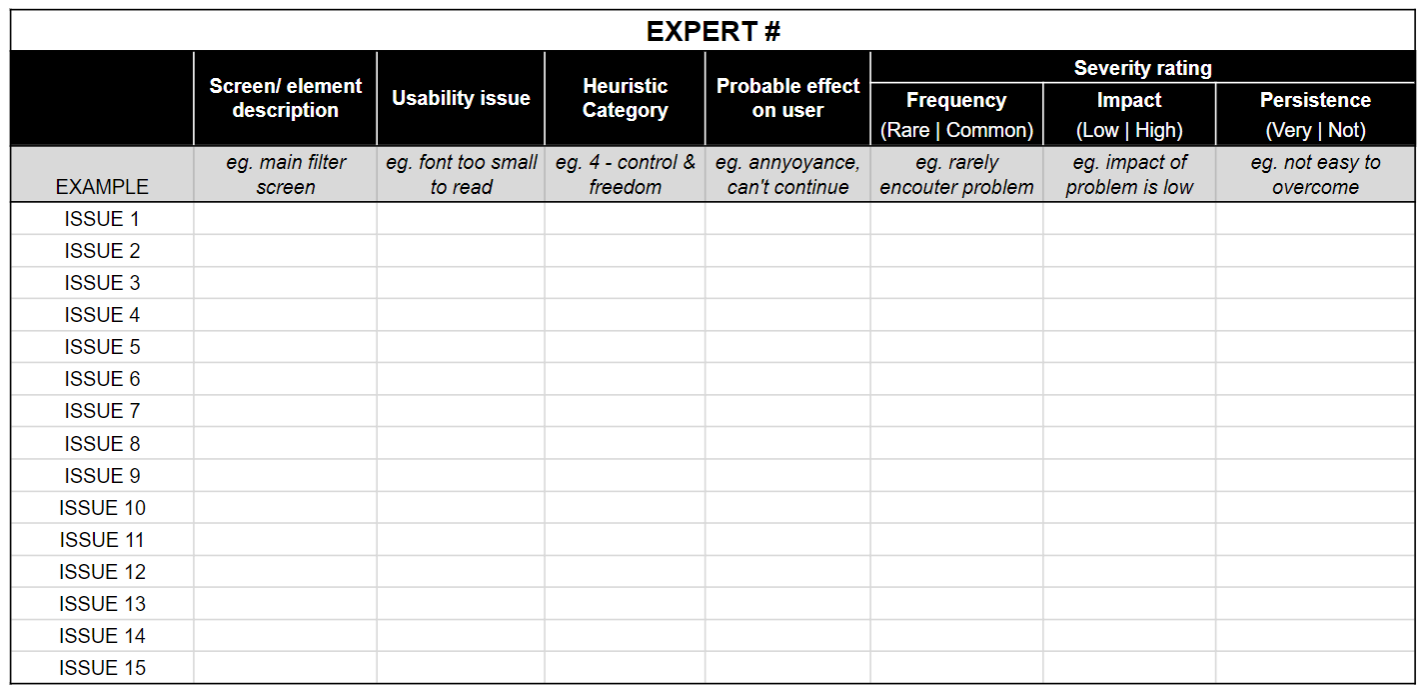
\includegraphics[width=0.9\textwidth, frame]
            {./High_Fidelity/High_Expert_Template.PNG}
    \end{figure}

    % Expert Notes
    \pagebreak     
    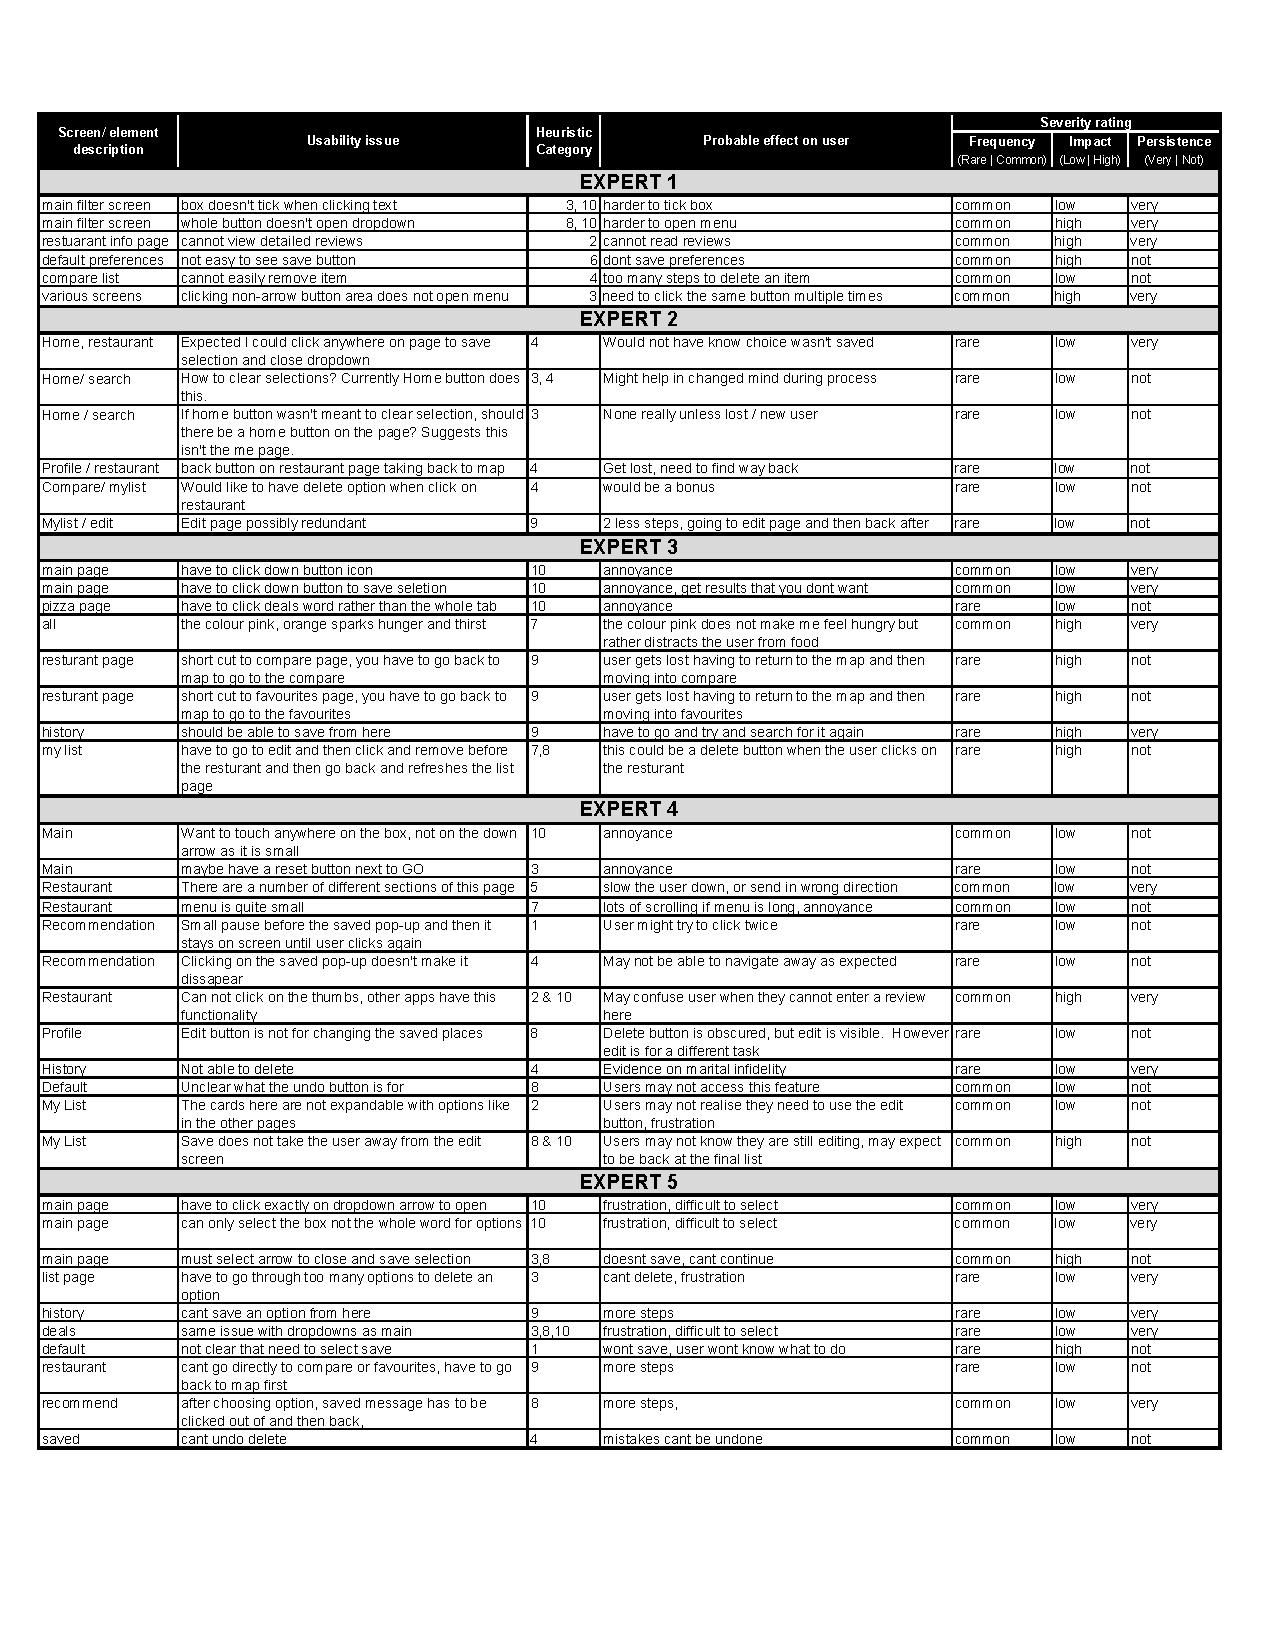
\includepdf[pages=1, 
                pagecommand=\subsection{Evaluation - Expert Notes}, 
                %width=\textwidth,
                %height=\textheight,
                keepaspectratio, offset= 0 -0.5cm]{High_Fidelity/High_Notes.pdf}
                \label{sec:C.5}


% CONCLUSION
% Title
\pagebreak
\begin{center}
    \vspace*{\stretch{0.7}}
    \Huge \textbf{Appendices}
    \section{Summary}
    \vspace*{\stretch{1}}
\end{center}


    % Conceptual Design
    \pagebreak     
    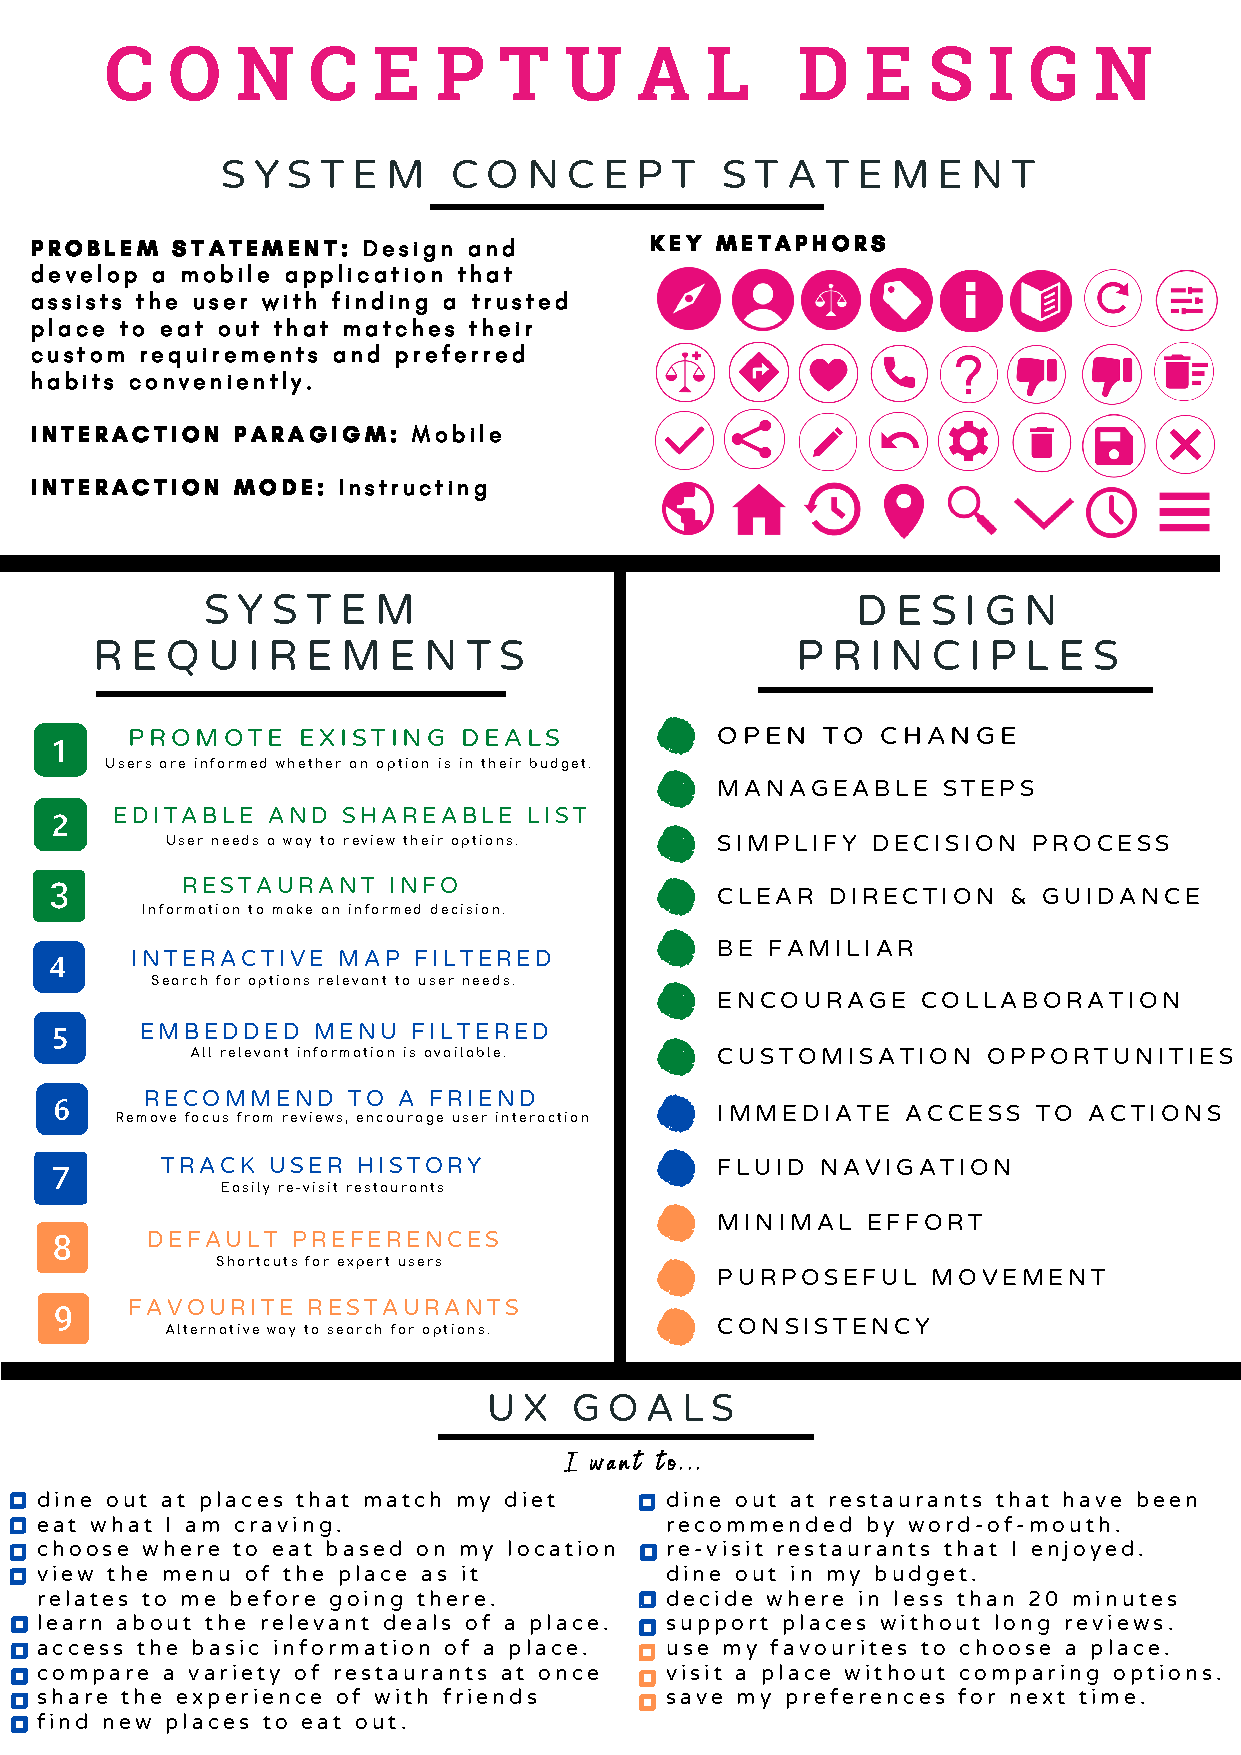
\includepdf[pages=1, 
                pagecommand=\subsection{Conceptual Design},              
                width=\textwidth,
                height=\textheight,
                keepaspectratio, 
                frame, offset= 0 -0.5cm]
                    {Summary/Conceptual_Design.pdf}
                    \label{sec:D.1}

    % Prototype Progression
    \pagebreak   
    \label{sec:D.2}  
    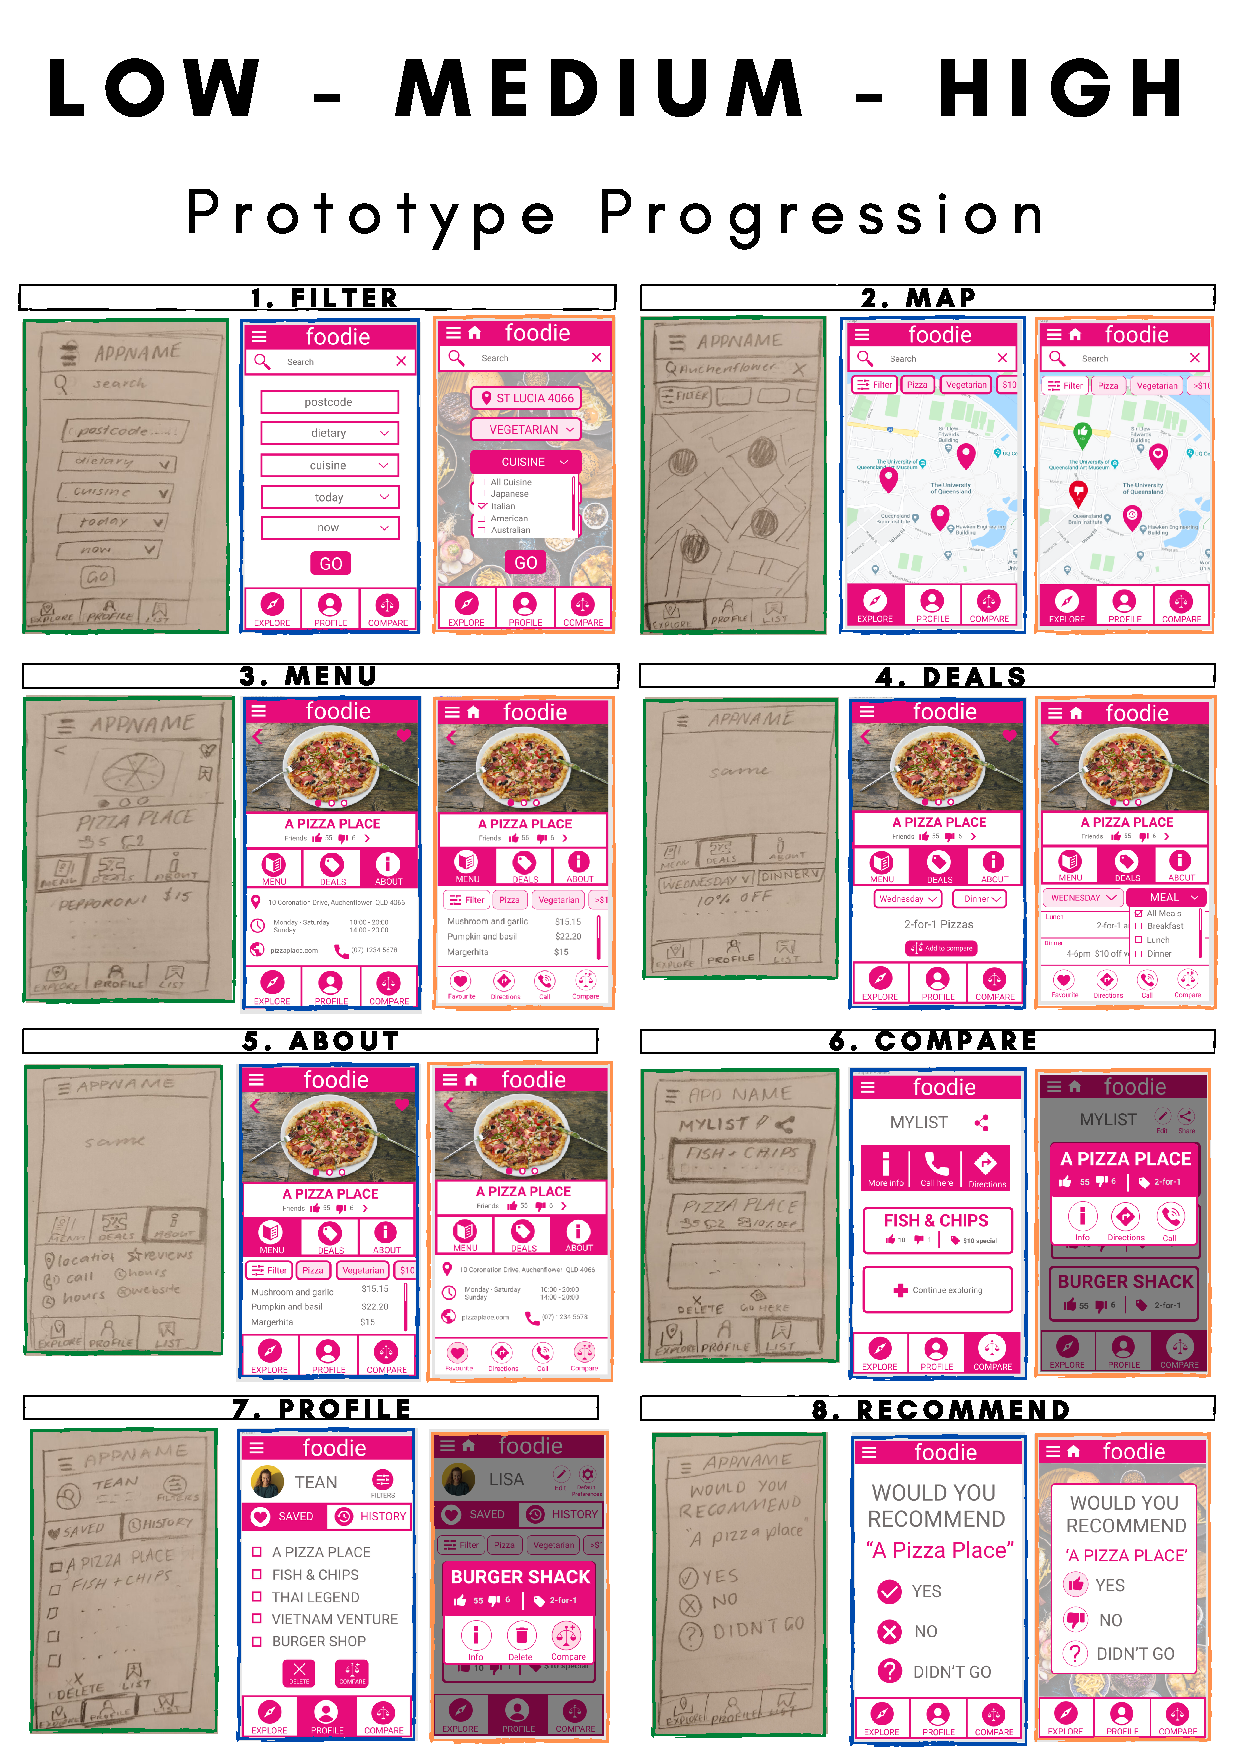
\includepdf[pages=1, 
                pagecommand=\subsection{Prototype Progression}, 
                width=\textwidth,
                height=\textheight,
                keepaspectratio, 
                frame, offset= 0 -0.5cm]
                    {Summary/Prototype_Progression.pdf}
                    

\end{document}